\documentclass[12pt,a4paper]{besnote}

\usepackage[utf8]{inputenc}
\DeclareUnicodeCharacter{2212}{-}

\usepackage{setspace}
\setstretch{1.15}

\usepackage{besphysics}
\usepackage{besrefblk}
\usepackage{authblk}
\usepackage[toc,page]{appendix}
\usepackage{fancyhdr}
\usepackage{graphicx}
\usepackage{float}
\usepackage{rotating}
%\floatstyle{boxed}
%\restylefloat{figure}
\usepackage{subfig}
\captionsetup[subfloat]{position=bottom}

\usepackage{overpic}
\usepackage{colortbl}
%\usepackage{epsfig}
%\usepackage{psfrag}
%\usepackage{pstricks}
\usepackage{amsfonts}
\usepackage{amsmath}
\usepackage{amssymb}
\usepackage{multirow}
\usepackage{multicol}
%\usepackage[square,comma,numbers,sort&compress]{natbib} % needed to order and compress multiple references%
\usepackage{diagbox}
\usepackage{units}
\usepackage{fancyhdr}
\usepackage{hangcaption}
\usepackage{xspace}
\usepackage{indentfirst}
\usepackage{hyperref}
%\usepackage[colorlinks,
%            linkcolor=blue,
%            anchorcolor=blue,
%            citecolor=blue
%            ]{hyperref}
%\usepackage[a4paper=true, pdfhighlight=/I, ps2pdf=true, dvips, dvipdfm ]{hyperref}
%\usepackage{hypernat}  %needed to let natbib with compress option work together with hyperref
%\usepackage{verbatim}

\usepackage{multicol}
\usepackage{graphicx}
\usepackage{booktabs}
\usepackage{amssymb,bm,mathrsfs,bbm,amscd}
\usepackage{lastpage}
\usepackage{geometry}
\usepackage{color}
\usepackage{tabularx}






\bibliographystyle{unsrtnat}

\usepackage{lineno}
%to avoid the hyphenation of Upper-case acronyms
\uchyph=0
\righthyphenmin=2
\lefthyphenmin=2

\hypersetup{
  breaklinks=true,
  colorlinks = true,
  linkcolor = blue,
  anchorcolor = blue,
  citecolor = blue,
  filecolor = blue,
  pagecolor = blue,
  urlcolor = blue
}
\hypersetup{
  bookmarks=true,
  bookmarksnumbered=true,
  bookmarkstype=toc,
  linktocpage=true
}

%\RequirePackage{lineno}

%\setlength{\parskip}{2ex}
\setlength{\parindent}{4ex}
\setlength{\oddsidemargin}{-0.5cm}
\setlength{\evensidemargin}{-0.5cm}
\setlength{\textwidth}{17cm}
\setlength{\topmargin}{-1cm}
\setlength{\textheight}{22cm}
\setlength{\headheight}{14pt}
\renewcommand{\arraystretch}{1}

% you can put a figure caption inside a table environment
% by command \figcaption.
% you can put a table caption inside a figure environment
% by command \tabcaption.
\makeatletter
    \newcommand\figcaption{\def\@captype{figure}\caption}
    \newcommand\tabcaption{\def\@captype{table}\caption}
\makeatother

\geometry{left=2.5cm,right=2.5cm,top=3cm,bottom=3.5cm}
%\newcommand{\xiaohao}{\fontsize{15pt}\baselineskip\linespread{0.5}\selectfont}

\title{Cross section measurement of process $\ee\to\pip\pim\piz$ from threshold to 2.0 GeV via ISR technique}

\author{
    Guang-Yan~Xiao~$^{a,c}$\footnote{E-mail:~{xiaogy@smail.nju.edu.cn}}~~
    Ya-Qian~Wang~$^{b}$~~
    Lei~Zhang~$^{a}$~~
    Shen-Jian~Chen~$^{a}$~~
    Chang-Zheng~Yuan~$^{c}$~~
    \\~\\
    $^a$Nanjing University\\
    $^b$Hebei University\\
    $^c$Institute of High Energy Physics, CAS\\
}

%Add the referee committee here

\refmember[d]{XXX (Chair)}
\refmember[e]{XXX}
\refmember[f]{XXX}
\refaffil[d]{\it XXX University}
\refaffil[e]{\it XXX University}
\refaffil[f]{\it XXX University}

\refeditor[g]{Editor A}
\refeditor[h]{Editor B}

\refbffil[g]{\it Uni. G}
\refbffil[h]{\it Uni. H}

% for the draft version
\besmemoversion{2.0} 

\besmemoid{xxx}

\date{\it \small \bf BESIII Analysis Memo (\today) }

%\pagestyle{fancy}
%\fancyhf{}
%\lhead{\nouppercase\leftmark}
%\cfoot{\thepage}


\abstracttext{ 
    XXX
}
\usepackage{perpage}  % 引入 perpage 包
\MakePerPage{footnote}  % 使脚注每页重新编号


\begin{document}

%\setpagewiselinenumbers
%\modulolinenumbers[2]
%\linenumbers

\section*{List of changes}
\label{sec:changes}

For an easy reading of the document, major changes in various versions with respect to the previous one are listed below.

\subsection*{Version 1.0}
\begin{itemize}
\item First version of memo.
\end{itemize}

\clearpage
\tableofcontents
\clearpage

%\setpagewiselinenumbers
%\modulolinenumbers[2]
%\linenumbers
\setrunninglinenumbers
\begin{linenumbers}

    % \input{table_test.tex}
    \section{Introduction}
\label{sec:intro}

The anomalous magnetic moment of the muon, \(a_\mu = (g-2)/2\), is a cornerstone quantity for testing the Standard Model (SM) and probing new physics. In 2025, the Muon \(g-2\) Experiment at Fermilab released its final measurement~\cite{Aguillard2025,Driutti2025} based on the complete Run 1--6 dataset, yielding a world average experimental value combining with the BNL E821 result~\cite{Bennett2006} of
\[
a_\mu^{\mathrm{exp}} = 116\,592\,072(1.5) \times 10^{-11} \quad (124\ \mathrm{ppb}).
\]

Within the Standard Model, \(a_\mu^{\mathrm{SM}}\) is decomposed into several contributions:
\[
a_\mu^{\mathrm{SM}} = a_\mu^{\mathrm{QED}} + a_\mu^{\mathrm{EW}} + a_\mu^{\mathrm{HVP}} + a_\mu^{\mathrm{HLbL}},
\]
where \(a_\mu^{\mathrm{QED}}\) denotes the quantum electrodynamics contribution (computed to five loops), \(a_\mu^{\mathrm{EW}}\) the electroweak contribution, \(a_\mu^{\mathrm{HVP}}\) the hadronic vacuum polarization, and \(a_\mu^{\mathrm{HLbL}}\) the hadronic light-by-light scattering. Among these, the hadronic contributions --- particularly \(a_\mu^{\mathrm{HVP}}\) --- dominate the theoretical uncertainty.

The largest uncertainty in the SM prediction comes from the leading-order hadronic vacuum polarization (LO-HVP) contribution, \(a_\mu^{\mathrm{HVP}}\), which cannot be computed perturbatively. In the traditional data-driven dispersive approach, \(a_\mu^{\mathrm{HVP}}\) is obtained via the dispersion integral~\cite{Brodsky1968,Lautrup1968}
\[
a_\mu^{\mathrm{HVP}} = \frac{\alpha^2}{3\pi^2} \int_{4m_\pi^2}^{\infty} \frac{ds}{s} K(s) \, R(s),
\]
where \(R(s) = \sigma(e^+e^-\to \mathrm{hadrons}) / \sigma(e^+e^-\to \mu^+\mu^-)\) is the hadronic \(R\)-ratio, and \(K(s)\) is a known QED kernel function that peaks at low energies. Consequently, high-precision measurements of exclusive hadronic cross sections at \(e^+e^-\) colliders are indispensable for a reliable SM prediction.

The WP2020~\cite{WP2020} evaluation by the Muon \(g-2\) Theory Initiative relied on this data-driven method. It yielded a SM prediction of
\[
a_\mu^{\mathrm{SM}}(\mathrm{WP2020}) = 116\,591\,810(43) \times 10^{-11},
\]
which, when compared with the then-available experimental value, resulted in a \(>5\sigma\) deviation, fueling intense interest in possible new physics.

However, the theoretical landscape has undergone a fundamental shift with the publication of the 2025 White Paper (WP2025)~\cite{WP2025}. Persistent tensions among different \(e^+e^-\to\pi^+\pi^-\) measurements --- in particular the higher \(\pi\pi\) cross section reported by the CMD-3 experiment~\cite{CMD3_Ignatov2024} compared to other earlier experiments --- have made it impossible to produce a meaningful combined data-driven average. In contrast, lattice QCD~\cite{Borsanyi2021} calculations of the LO-HVP have reached sub-percent precision and show good internal consistency among different collaborations.

Consequently, WP2025 adopts a consolidated lattice-QCD average as its central value for the LO-HVP contribution, rather than the data-driven result used in WP2020. This change shifts the total SM prediction upward to
\[
a_\mu^{\mathrm{SM}}(\mathrm{WP2025}) = 116\,592\,033(62) \times 10^{-11}.
\]

The comparison between theory and experiment now yields:
\[
a_\mu^{\mathrm{exp}} - a_\mu^{\mathrm{SM}}(\mathrm{WP2025}) = 38(63) \times 10^{-11},
\]
corresponding to a negligible deviation of approximately \(0.6\sigma\). The long-standing \(>5\sigma\) discrepancy has effectively been resolved with the updated SM prediction. Nevertheless, this resolution does not imply that the problem is fully understood. The disagreement between the data-driven and lattice-QCD evaluations of the LO-HVP term remains unresolved, as does the tension between CMD-3 and other \(e^+e^-\to\pi^+\pi^-\) experiments. Resolving these discrepancies requires new, independent, high-precision measurements of the key hadronic cross sections, particularly those with the largest contributions to \(a_\mu^{\mathrm{HVP}}\).

% Among all exclusive channels, the \(2\pi\) final state dominates, contributing \(\sim 70\%\) of the total HVP. The second most important channel is \(e^+e^-\to\pi^+\pi^-\pi^0\) (\(3\pi\)), which contributes \(\sim 10\%\) but is a major source of systematic uncertainty due to its complex resonance structure (dominated by \(\omega\) and \(\phi\)). 

For the \(3\pi\) channel, the Belle II experiment reported a new measurement in 2024~\cite{BelleII_3pi_2024}. However, concerns have been raised regarding the reliability of its uncertainty estimation, leading some recent SM theory compilations to explicitly exclude Belle II data from their averages\cite{Hoferichter2025}. This situation highlights the urgent need for independent cross section measurements from other facilities.

The BESIII experiment, with its large data samples, is ideally suited to provide a reliable and independent measurement of the \(e^+e^- \to \pi^+\pi^-\pi^0\) cross section in the low-energy region critical for \(a_\mu^{\mathrm{HVP}}\). In this memo, we use an \(e^+e^-\) collision sample corresponding to an integrated luminosity of 20~fb\(^{-1}\) collected at a center-of-mass energy of 3.773~GeV. We present a measurement based on the initial-state radiation (ISR) technique using the process \(e^+e^- \to \pi^+\pi^-\pi^0 \gamma_{\mathrm{ISR}}\), which allows access to the \(3\pi\) hadronic cross section from continuum production without energy scanning. This work aims to provide a valid and systematically well-controlled measurement, thereby adding reliable experimental input for the \(3\pi\) channel and contributing to the ongoing effort to reconcile the data-driven and lattice-QCD approaches.
    % \clearpage
\section{BEPCII and BESIII detector}
\label{sec:detector}
The Beijing Electron-Positron Collider II (BEPCII) \textemdash a double-ring multi-bunch collider \textemdash is operating in the \(\rm \tau\)-charm energy region (1.84 to 4.95 GeV) with the design luminosity of \(\rm 1\times10^{33}~cm^{-2}s^{-1}\)~\cite{whitePaper}. The Beijing Spectrometer III (BESIII) operating at BEPCII is a high-precision, general-purpose detector that records symmetric $\ee$ collisions provided by the BEPCII storage ring. BESIII is approximately cylindrically symmetric with 93\% coverage of the solid angle around the $\ee$ interaction point (IP). The components of the apparatus ordered by distance from the IP, are a 43-layer small-cell main drift chamber (MDC), a time-of-flight (TOF) system based on plastic scintillators with two layers in the barrel region and one layer in the end-cap region (the end-cap TOF system has been updated with the multi-gap resistive plate chamber in 2014~\cite{Yang2014}), a 6240-cell CsI(Tl) crystal electromagnetic calorimeter (EMC), a superconducting solenoid magnet providing a 1.0 T magnetic field aligned with the beam axis, and resistive plate muon-counter layers interleaved with steel. The momentum resolution for charged tracks in the MDC is 0.5\% for transverse momenta with 1 GeV/c. The energy resolution in the EMC is 2.5\% in the barrel region and 5.0\% in the end-cap region for 1 GeV photons. For charged tracks, particle identification (PID) for charged tracks combines measurements of the energy deposit dE/dx in MDC and flight time in TOF and forms likelihoods $\mathcal{L}(h)(h=K, \pi)$ for a hadron $h$ hypothesis. More details about the BESIII detector are provided in Ref~\cite{BESIII_detector}.
 
    \clearpage
\section{Data and MC samples}
\label{sec:sample}
We use an $\ee$ collision sample corresponding to an integrated luminosity of 20 $\ifb$, collected by BESIII detector at center-of-mass energy of 3.773 $\gev$, under BOSS-7.1.2 version. The details are listed in Table~\ref{tab:datalumi}, quoted from Ref.~\cite{BESIII_lumi0304, BESIII_lumi_2024}.

\begin{table}[t]
    \begin{center}
        \caption{Beam energies and integrated luminosities of the data samples used in this work, quoted from Ref.~\cite{BESIII_lumi0304, BESIII_lumi_2024}.}
        \vspace{4mm}
        \begin{tabular}{c | c | c | c}
            \hline \hline

            $E_{\text{beam}} (\rm GeV)$            & Integrated luminosity
            ($\text{pb}^{-1}$)                     & Data taking time                               & RunNo                          \\
            \hline
            3.773                                  & \( 2931.8 \pm
            0.2 \pm 13.8 \)~\cite{BESIII_lumi0304} & 2010(round03)                                  & 11414 -- 13988, 14395 -- 14604 \\                                                         &                                                                                    &
            2011(round04)                          & 20448 -- 23454                                                                  \\
            \hline
            3.773                                  & \( 4995.0 \pm 19.0 \) ~\cite{BESIII_lumi_2024} &
            2022(round15)                          & 70522 -- 73929                                                                  \\
            \hline
            3.773                                  & \( 8157.0 \pm 31.0 \) ~\cite{BESIII_lumi_2024} &
            2023(round16)                          & 74031 -- 78536                                                                  \\
            \hline
            3.773                                  & \( 4191.0 \pm 16.0 \) ~\cite{BESIII_lumi_2024} &
            2024(round17)                          & 78615 -- 81094                                                                  \\
            % \hline
            % 4.178                       & \( 3195.0 \pm 32.0 \) [19]     &
            % 2016                        & 43716 -- 45105, 45418 -- 47066                                  \\ 
            \hline \hline
        \end{tabular}
        \label{tab:datalumi}
    \end{center}
\end{table}

Simulated Monte Carlo (MC) samples are employed to study backgrounds, optimize event selection, and estimate detection efficiencies. Two categories of MC samples are utilized in this analysis:

\begin{table}[t]
    \begin{center}
        \caption{Processes and luminosity scales of the inclusive MC samples used in this analysis. Separate samples are available for each data-taking round. Most processes use samples with an integrated luminosity equivalent to ten times that of the data.}
        \vspace{4mm}
        \begin{tabular}{l c}
            \hline \hline
            Process                                         & Luminosity scale \\
            \hline
            $e^+e^- \to \psi(3770) \to D^0\bar{D}^0$        & 10 $\times$      \\
            $e^+e^- \to \psi(3770) \to D^+D^-$              & 10 $\times$      \\
            $e^+e^- \to \tau^+\tau^-$                       & 10 $\times$      \\
            $e^+e^- \to \psi(3770) \to \text{non-}D\bar{D}$ & 10 $\times$      \\
            $e^+e^- \to q \bar{q}$                          & 10 $\times$      \\
            $e^+e^- \to \gamma_{\text{ISR}} \psi(2S)$       & 10 $\times$      \\
            $e^+e^- \to \gamma_{\text{ISR}} J/\psi$         & 10 $\times$      \\
            $e^+e^- \to e^+e^-$                             & 0.25 $\times$    \\
            $e^+e^- \to \gamma \gamma$                      & 3 $\times$       \\
            $e^+e^- \to \mu^+\mu^-$                         & 15 $\times$      \\
            \hline \hline
        \end{tabular}
        \label{tab:inclusiveMC_processes}
    \end{center}
\end{table}

\begin{itemize}
    \item \textbf{The inclusive MC samples} comprehensively model known physics processes at $\sqrt{s}=3.773\gev$, including $D\bar{D}$ production, $\tau^+\tau^-$ pair production, initial-state-radiation (ISR) production of vector charmonium states ($J/\psi$ and $\psi(2S)$), QED processes, and continuum light hadron production. The charm working group provides separate samples for the different data-taking rounds(round03-04, round15, round16, and round17)~\cite{BESIII_MEMO_INCLUSIVE}. In this analysis, we use inclusive MC samples with an integrated luminosity equivalent to ten times that of the data for most processes, except for the QED processes $e^+e^- \to e^+e^-$, $\gamma \gamma$, and $\mu^+\mu^-$, where we use the samples with the scaling factors provided by the charm working group. The processes and the corresponding luminosity scales of the samples used in this analysis are summarized in Table~\ref{tab:inclusiveMC_processes}.

    \item \textbf{Exclusive signal and background MC samples} generated specifically for this analysis using the \textsc{PHOKHARA} event generator~\cite{Czyz2006,Rodrigo2001,Rodrigo2002} (version 9.1). These samples are produced independently for each data-taking round (round03, round04, round15, round16, round17) to account for variations in detector conditions. Sufficient statistics are generated for each process to ensure reliable efficiency determination and background studies. The generated processes include:
          \begin{itemize}
              \item $\ee\to \pi^+\pi^-\pi^0\gamma_{\text{ISR}}$ (signal process)
              \item $\ee\to \pi^+\pi^-\pi^0\pi^0$
              \item $\ee\to \pi^+\pi^-\pi^0\pi^0\gamma_{\text{ISR}}$
          \end{itemize}
          These exclusive samples are used for signal efficiency studies, background characterization, and validation of the analysis methodology.
\end{itemize}
    \clearpage
\section{Event Selections}
\label{sec:selections}
The process under investigation is $e^{+} e^{-} \rightarrow \pip\pim\piz \gamma_{\mathrm{ISR}}$, whose final states include two charged tracks, one neutral $\piz$, and one ISR photon. The following selection criteria is applied to all the data samples. Here the figures are shown by taking $\sqrt{s}=3.773 \mathrm{GeV}$ round16 data as an example. The distributions related to the event selection of other data sets are shown in Appendix. XXX. Situations are similar to each other.


\begin{itemize}
    \item Good charged track:
          A charged track is taken as a good MDC track if it originates from the beam vertex and lies within the MDC polar angle region:
          \begin{itemize}
              \item $|\cos\theta|<0.93$, where $\theta$ is the polar angle with respect to the beam axis.
              \item $|\Delta r|<1\,\unit{cm}$, $|\Delta z|<10\,\unit{cm}$, where $|\Delta r|$ and $|\Delta z|$ is distance of closest approach to the interaction point (IP) perpendicular to the beam axis and along the beam axis, respectively.
              \item  the ratio of the calorimeter-deposited energy to the track momentum $E_{EMC}/p$ is required to be less than 0.8 for both of the charged tracks.
              \item no PID requirements for $\pip$, $\pim$.
          \end{itemize}

          % \item PID requirement:
          %       d$E$/d$x$ and TOF informations are combined to form the PID confidence level for protons, pions and kaons, respectively. $p^\pm$ is identified with:
          %       \begin{itemize}
          %           \item $p$ PID requirements: $\mathcal{L}$($p$)$>$0 $\mathcal{\&\&}$ $\mathcal{L}$($p$)$>$$\mathcal{L}$($K$) $\mathcal{\&\&}$ $\mathcal{L}$($p$)$>$$\mathcal{L}$($\pi$).
          %                 %   \item $K$ PID requirements: prob($K$)$>$0 $\mathcal{\&\&}$ prob($K$)$>$prob($\pi$).
          %                 %   \item $\pi$ PID requirements:  prob($\pi$)$>$0 $\mathcal{\&\&}$ prob($\pi$)$>$prob($K$).
          %       \end{itemize}

    \item $\gamma$ selection:
          \begin{itemize}
              \item $E>0.025\gev$~(barrel: $|\cos\theta|<0.8$), $E>0.050\gev$~(endcap: $0.86<|\cos\theta|<0.92$).
              \item $0\leqslant t_{\rm TDC} \leqslant 14$($\times 50 \unit{ns}$) to suppress fake photons due to electronic noise or beam background.
              \item the closest angle with all charged tracks $\theta>10^{\circ}$ to suppress background from radiation of charged tracks.
          \end{itemize}
    \item $\piz \to \gamma\gamma$ selection:
          \begin{itemize}
              \item two photon invariant mass $M_{\gamma\gamma}$ within (0.115, 0.150)$\gevcc$.
              \item To improve the momentum resolution, 1C kinematic fit is performed. Here, the 1C means $\piz$ mass constraint, and the updated 4-momentum will be used in the further analysis. $\chi^2_{\mathrm{KF}}<10$
          \end{itemize}
\end{itemize}

Candidate events are selected by requiring exactly two good charged tracks, accompanied by at least one reconstructed $\pi^0$ and a minimum of three good photon showers. This ensures the presence of at least one $\pi^0$ and one isolated photon from Initial-State Radiation ($\gamma_{\mathrm{ISR}}$). A four-constraint (4C) kinematic fit is then applied to the event, and the candidate with the smallest $\chi_{\mathrm{4C}}^2$ value is chosen for further analysis.

After identifying an ISR photon from the isolated photon showers, the invariant mass of the remaining $e^+e^- \to \pi^+\pi^-\pi^0$ system is reconstructed. As expected for ISR processes, the resulting center-of-mass energy $\sqrt{s'}$ of the $\pi^+\pi^-\pi^0$ system shows a continuous spectrum, characteristic of the radiative return mechanism. This continuum behavior is illustrated in Fig.~\ref{fig:signal_mc_mass_spectra} across the $\omega(782)$, $\phi(1020)$, and $\omega^{\prime}/\omega^{\prime\prime}$ mass regions.

\begin{figure}[H]
    \centering
    \subfloat[$\omega(782)$ region]{
        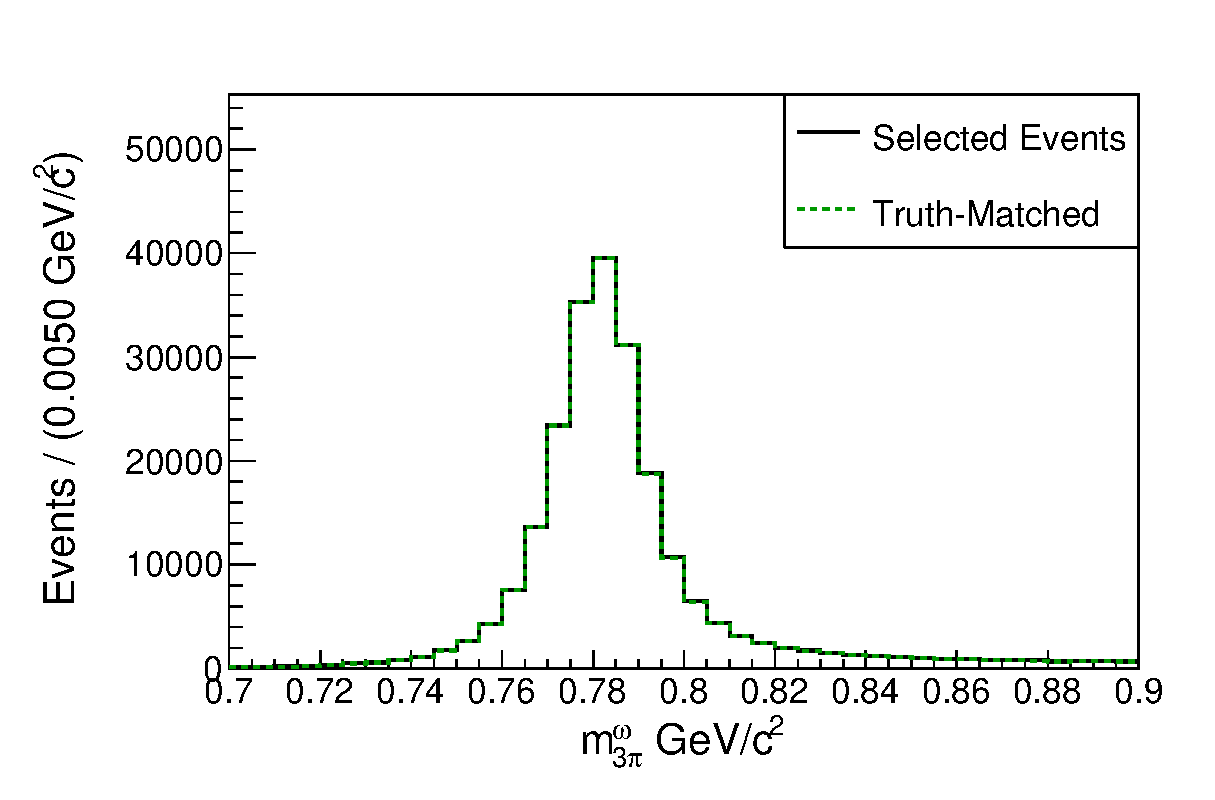
\includegraphics[width=0.32\textwidth]{fig/hist_omega_region_with_truth.eps}
        \label{fig:mc_mass_omega_region}
    }
    \hfill
    \subfloat[$\phi(1020)$ region]{
        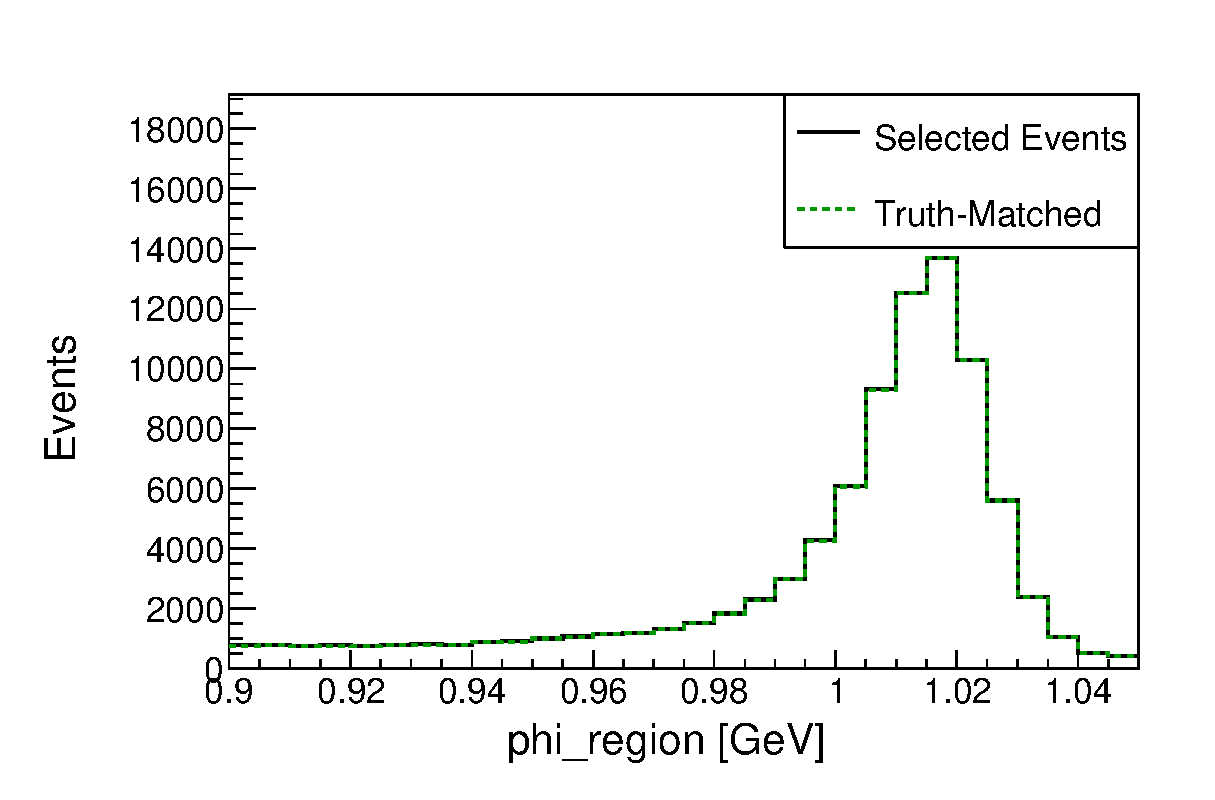
\includegraphics[width=0.32\textwidth]{fig/hist_phi_region_with_truth.eps}
        \label{fig:mc_mass_phi_region}
    }
    \hfill
    \subfloat[$\omega^{\prime}$ and $\omega^{\prime\prime}$ region]{
        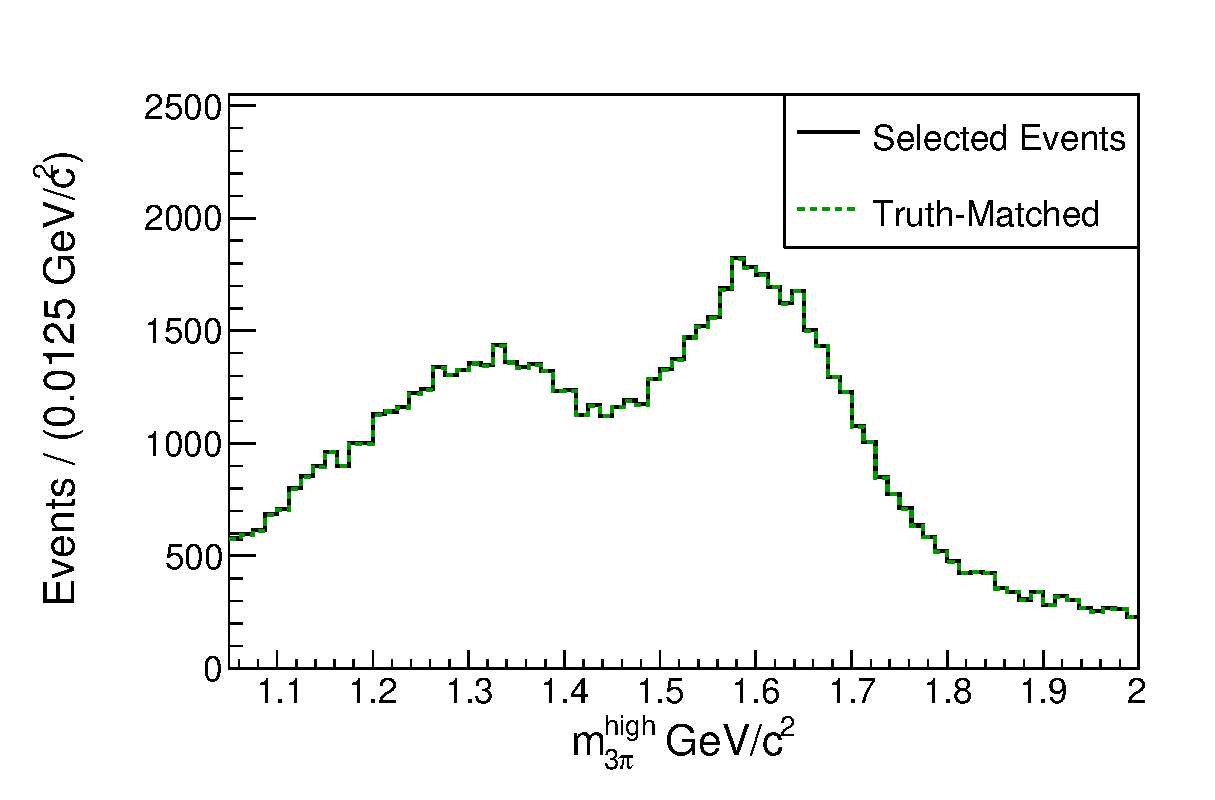
\includegraphics[width=0.32\textwidth]{fig/hist_omegap_region_with_truth.eps}
        \label{fig:mc_mass_omegap_region}
    }

    \caption{Invariant mass spectra of MC in the (a) $\omega(782)$, (b) $\phi(1020)$, and (c) $\omega^{\prime}/\omega^{\prime\prime}$ mass regions. The distributions correspond to $M(pK_S^0)$, $M(p\pi^0)$, and $M(K_S^0\pi^0)$, respectively. The "Truth-Matched" distribution (green dashed line) corresponds to reconstructed events where the momentum directions of the $\pi^0$ and $\gamma_{\mathrm{ISR}}$ successfully match their truth-level counterparts. A loose requirement of $\chi^2_{\text{KF}} < 100$ is applied to the kinematic fit. The continuous spectrum of $\sqrt{s'}$ for the $\pi^+\pi^-\pi^0$ system demonstrates the radiative return mechanism via ISR. }
    \label{fig:signal_mc_mass_spectra}
\end{figure}
    
\clearpage
\section{Background Study}
\label{sec:bkg_stu}
In the study of background processes, the main backgrounds are categorized into $e^{+}e^{-} \to \pi^{+}\pi^{-}\pi^{0}\pi^{0}$, $e^{+}e^{-} \to \pi^{+}\pi^{-}\pi^{0}\pi^{0}\gamma_{\text{ISR}}$, QED processes, and others. The dominant contributions arise from processes with additional $\pi^{0}$, particularly $e^{+}e^{-} \to \pi^{+}\pi^{-}\pi^{0}\pi^{0}$, while $e^{+}e^{-} \to \pi^{+}\pi^{-}\pi^{0}\pi^{0}\gamma_{\text{ISR}}$ is not dominant but shares the same underlying mechanism as a background to our signal. In the inclusive analysis, the cross sections used for these two processes were not correctly configured.

To verify that these processes constitute the primary backgrounds, the
$\mathcal{L} \times \sigma_{\text{hadron}}$ method is employed, where
$\mathcal{L}$ is the integrated luminosity and $\sigma_{\text{hadron}}$ is the
hadronic cross section. The luminosity values for each data-taking period are
listed in Table~\ref{tab:datalumi}. The background yield is estimated as a
function of the $\pi^{+}\pi^{-}\pi^{0}$ invariant mass ($m$) using the
effective luminosity spectrum, which is related to the mass spectrum via:

\begin{equation}
    \frac{d L_{\text{eff}}}{d m} = \frac{2 m}{s} \cdot F(s, m) \cdot \mathcal{L}_{\text{int}},
\end{equation}

where $s = 4E^{2}$, $E$ is the beam energy, $\mathcal{L}_{\text{int}}$ is the
total integrated luminosity, and $F(s, m)$ is the probability function for
initial-state photon emission. This function can be written
as~\cite{Kuraev1985}:

\begin{align}
    \beta                        & = \frac{2\alpha}{\pi} \left[ \ln\left( \frac{s}{m_e^{2}} \right) - 1 \right],                                                                              \\
    x                            & = 1 - \frac{m^{2}}{s},                                                                                                                                     \\
    \frac{d L_{\text{eff}}}{d m} & = \frac{2 m}{s} \cdot \Bigg\{ \beta x^{\beta-1} \Bigg[ 1 + \frac{\alpha}{\pi} \left( \frac{\pi^{2}}{3} - \frac{1}{2} \right) + \frac{3}{4} \beta \nonumber \\
                                 & \quad + \beta^{2} \left( \frac{37}{96} - \frac{\pi^{2}}{12} - \frac{1}{72} \ln \frac{s}{m_e^{2}} \right) \Bigg] \nonumber                                  \\
                                 & \quad - \beta \left(1 - \frac{x}{2}\right) \ln\frac{1}{x} - \frac{1+3(1-x)^{2}}{x} \ln(1-x) - 6 + x \Bigg\} \cdot \mathcal{L}_{\text{int}},
\end{align}

where $\alpha = 1/137$ is the fine-structure constant, $m_e = 0.5110034 \times
    10^{-3}~\text{GeV}/c^{2}$ is the electron mass, and $\sqrt{s} =
    3.773~\text{GeV}$ is the center-of-mass energy of the primary $e^{+}e^{-}$
system.

The effective luminosity spectrum calculated using this formula for round16 is
shown in Fig.~\ref{fig:luminosity_spectrum}. Similar calculations were
performed for all data-taking rounds.

\begin{figure}[htbp]
    \centering
    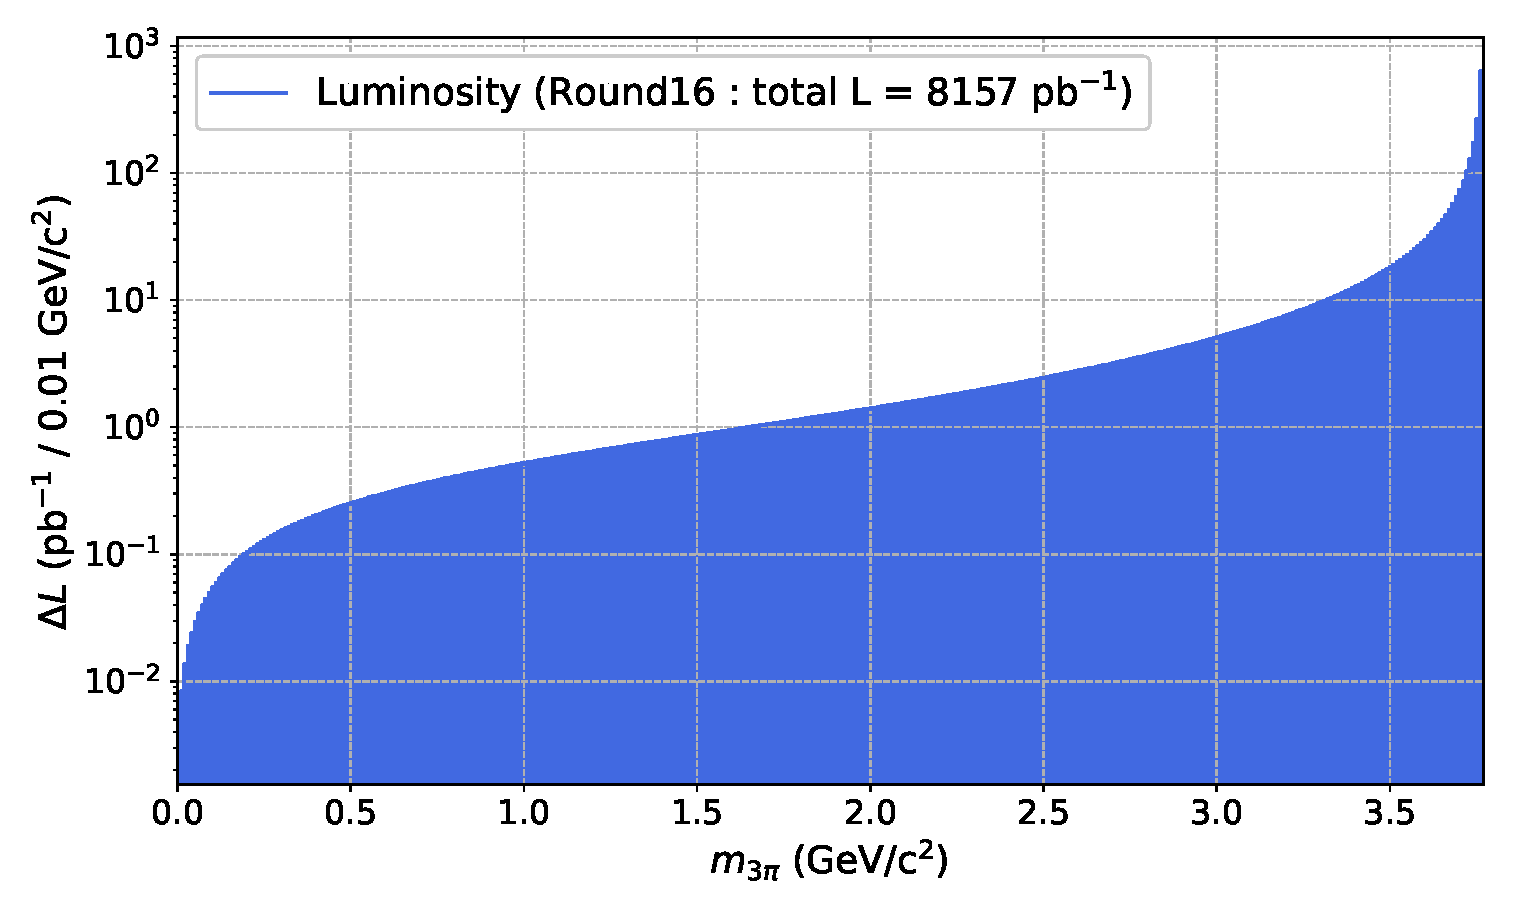
\includegraphics[width=0.45\textwidth]{fig/luminosity_spectrum.eps}
    \caption{Effective luminosity spectrum as a function of the $\pi^{+}\pi^{-}\pi^{0}$ invariant mass ($m_{3\pi}$) calculated for round16 with total integrated luminosity $\mathcal{L}_{\text{int}} = 8157~\text{pb}^{-1}$. The spectrum is shown with logarithmic scale on the vertical axis.}
    \label{fig:luminosity_spectrum}
\end{figure}

Based on this method, rough yield estimates for the two processes with
additional $\pi^{0}$, $e^{+}e^{-} \to \pi^{+}\pi^{-}\pi^{0}\pi^{0}$ (non-ISR)
and $e^{+}e^{-} \to \pi^{+}\pi^{-}\pi^{0}\pi^{0}\gamma_{\text{ISR}}$ (ISR),
were calculated for the four data-taking periods (round03/04, round15, round16,
round17). The results are summarized in
Table~\ref{tab:background_yield_estimate}. For the ISR channel, the estimation
relies on the $e^{+}e^{-} \to \pi^{+}\pi^{-}\pi^{0}\pi^{0}$ cross section
measured by the BaBar collaboration~\cite{BaBar2017_4pi0}.

It is important to note that the values listed in the table are initial yield
estimates without any selection efficiency corrections; the actual background
contribution to the signal region is obtained by multiplying these yields by
the corresponding selection efficiency relevant to the specific analysis cuts.
These estimates serve only to confirm that these processes constitute the main
sources of background and to provide guidance for optimizing subsequent
selection criteria.

\begin{table}[t]
    \begin{center}
        \caption{Rough estimates of the expected yields for the two processes with additional $\pi^{0}$ before applying any selection efficiency. The integrated luminosities are taken from Table~\ref{tab:datalumi}. The cross section for $e^{+}e^{-} \to \pi^{+}\pi^{-}\pi^{0}\pi^{0}$ is taken as $\sigma = 0.22$~nb at $\sqrt{s}=3.773$~GeV, while the energy-dependent cross section for the ISR process is derived from the measured $e^{+}e^{-} \to \pi^{+}\pi^{-}\pi^{0}\pi^{0}$ cross section~\cite{BaBar2017_4pi0}. The final background contribution is obtained by multiplying these yields by the corresponding selection efficiency.}
        \vspace{4mm}
        \begin{tabular}{c | c | c}
            \hline \hline
            Data sample (Run period) & $N(e^{+}e^{-} \to \pi^{+}\pi^{-}\pi^{0}\pi^{0})$ & $N(e^{+}e^{-} \to \pi^{+}\pi^{-}\pi^{0}\pi^{0}\gamma_{\text{ISR}})$ \\
            \hline
            round03-04               & 511940                                           & 1142096                                                             \\
            \hline
            round15                  & 872209                                           & 1945825                                                             \\
            \hline
            round16                  & 1424346                                          & 3177597                                                             \\
            \hline
            round17                  & 731817                                           & 1632623                                                             \\
            \hline \hline
        \end{tabular}
        \label{tab:background_yield_estimate}
    \end{center}
\end{table}

The final background yield is then obtained by multiplying the effective
luminosity spectrum by the cross section and a selection-efficiency factor that
varies dynamically with the analysis cuts. This method is used solely to
confirm that $e^{+}e^{-} \to \pi^{+}\pi^{-}\pi^{0}\pi^{0}$ and $e^{+}e^{-} \to
    \pi^{+}\pi^{-}\pi^{0}\pi^{0}\gamma_{\text{ISR}}$ are the dominant backgrounds
and to optimize the selection criteria. It is not used to derive the final
background estimates; precise yields for these two components will be
determined using data-driven methods.
Based on the rough background estimate from $\mathcal{L} \times
\sigma_{\text{hadron}}$, the signal yield was approximated by subtracting the
background from the data, allowing for a preliminary significance calculation.
Using this approach, a figure of merit (FOM) defined as $S / \sqrt{S + B}$ was
constructed to evaluate the signal significance. To optimize the event
selection, a scan over the kinematic fit $\chi^2$ was performed, with the
result for Round~16 shown in Fig.~\ref{fig:chisq_optimization_round16}.  
The Round~16 optimization yields an optimal cut of $\chi^{2}_{\mathrm{KF}} < 50$. 
As shown in Fig.~\ref{fig:chisq_optimization_rounds}, consistent convergence of 
significance is also observed for Rounds~03/04, 15, and 17 with the same cut.

\begin{figure}[htbp]
    \centering
    \subfloat[$\chi^2$ distribution for the 4C kinematic fit]{
        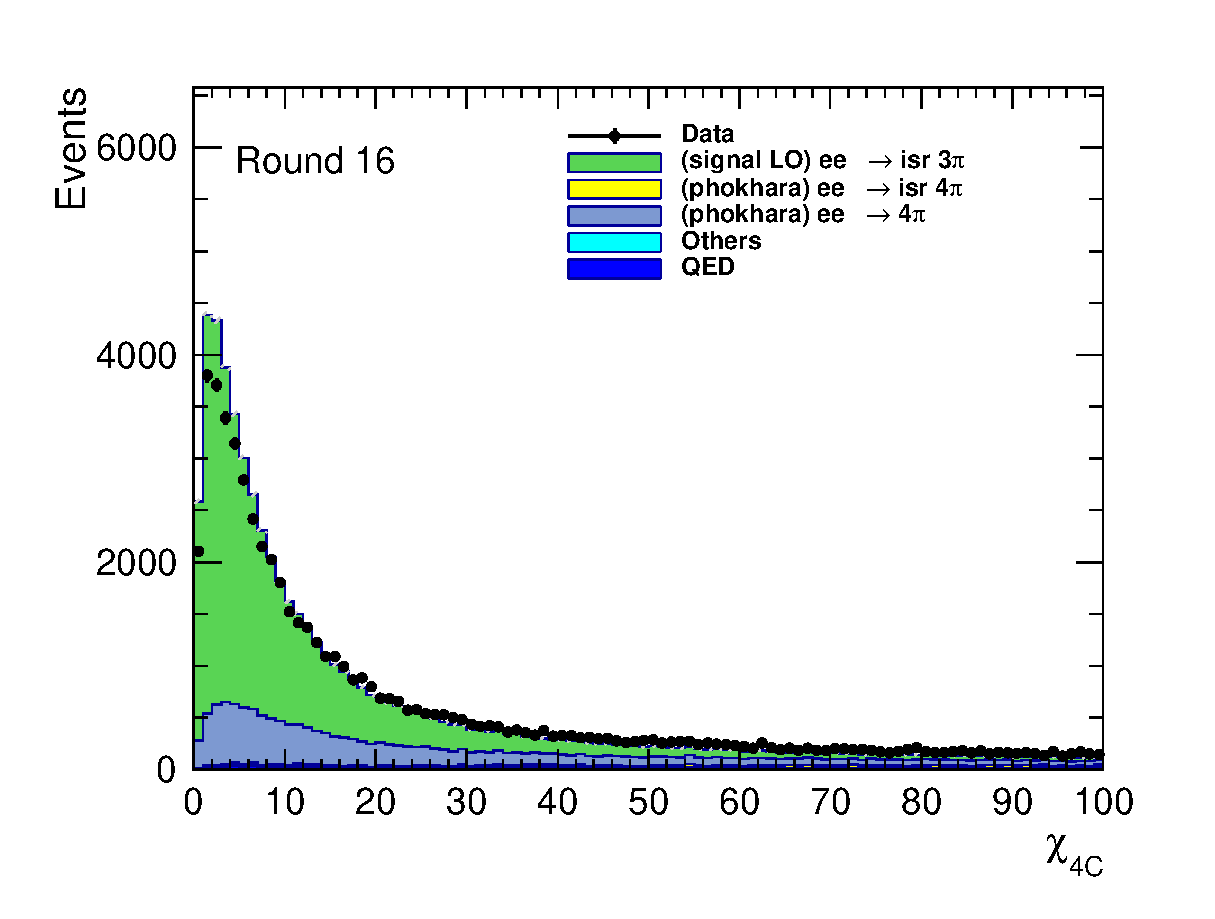
\includegraphics[width=0.48\textwidth]{fig/kmfitchisq_round16.eps}
        \label{fig:kmfitchisq_round16}
    }
    \hfill
    \subfloat[FOM scan as a function of the $\chi^2$ cut]{
        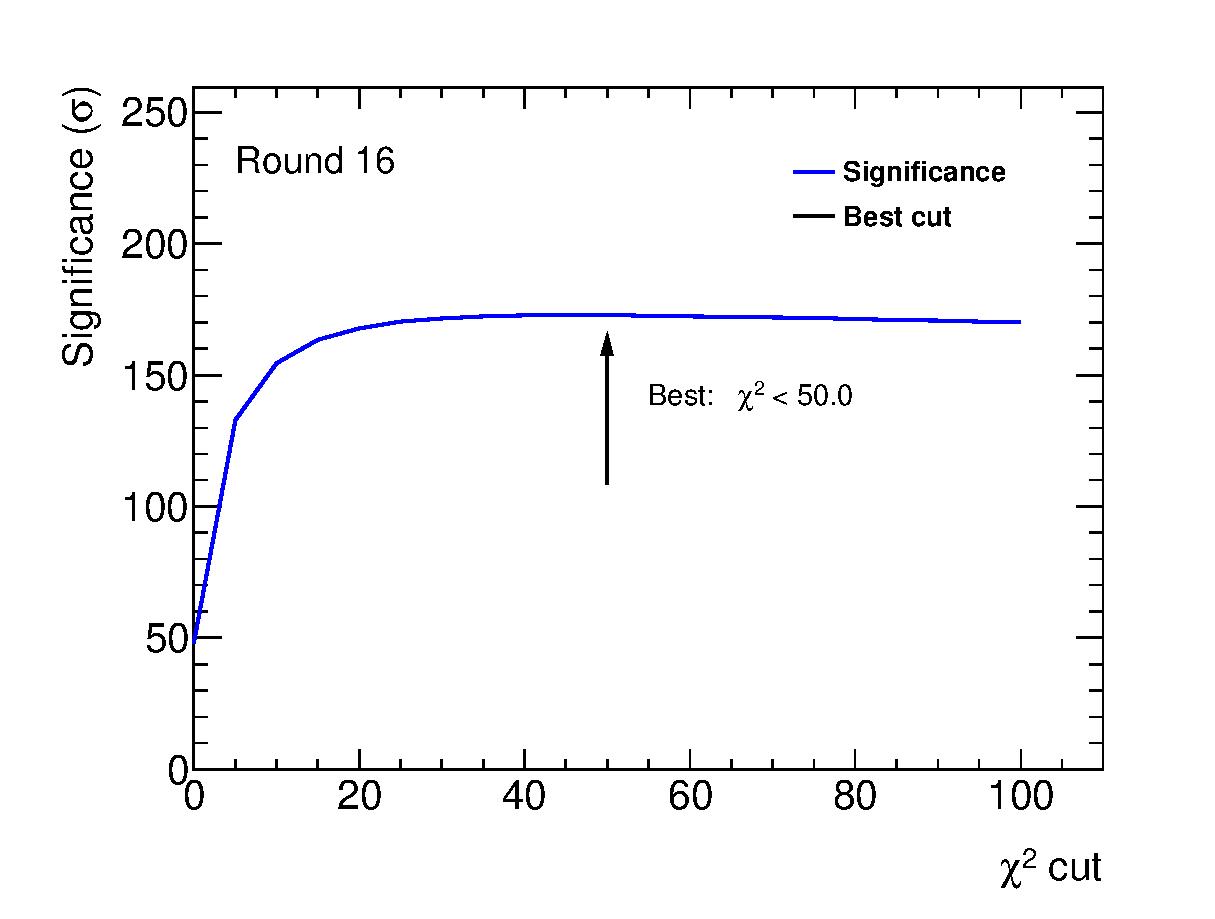
\includegraphics[width=0.48\textwidth]{fig/OptimizeChisq4C_scan_round16.eps}
        \label{fig:optimize_chisq_scan_round16}
    }
    \caption{(a) Distribution of the kinematic fit $\chi^2$ for the four-constraint (4C) fit using the Round~16 data sample. (b) The corresponding figure of merit ($S/\sqrt{S+B}$) as a function of the applied $\chi^2$ cut value for the Round~16 data.}
    \label{fig:chisq_optimization_round16}
\end{figure}

\begin{figure}[htbp]
    \centering
    \subfloat[Round 03/04]{
        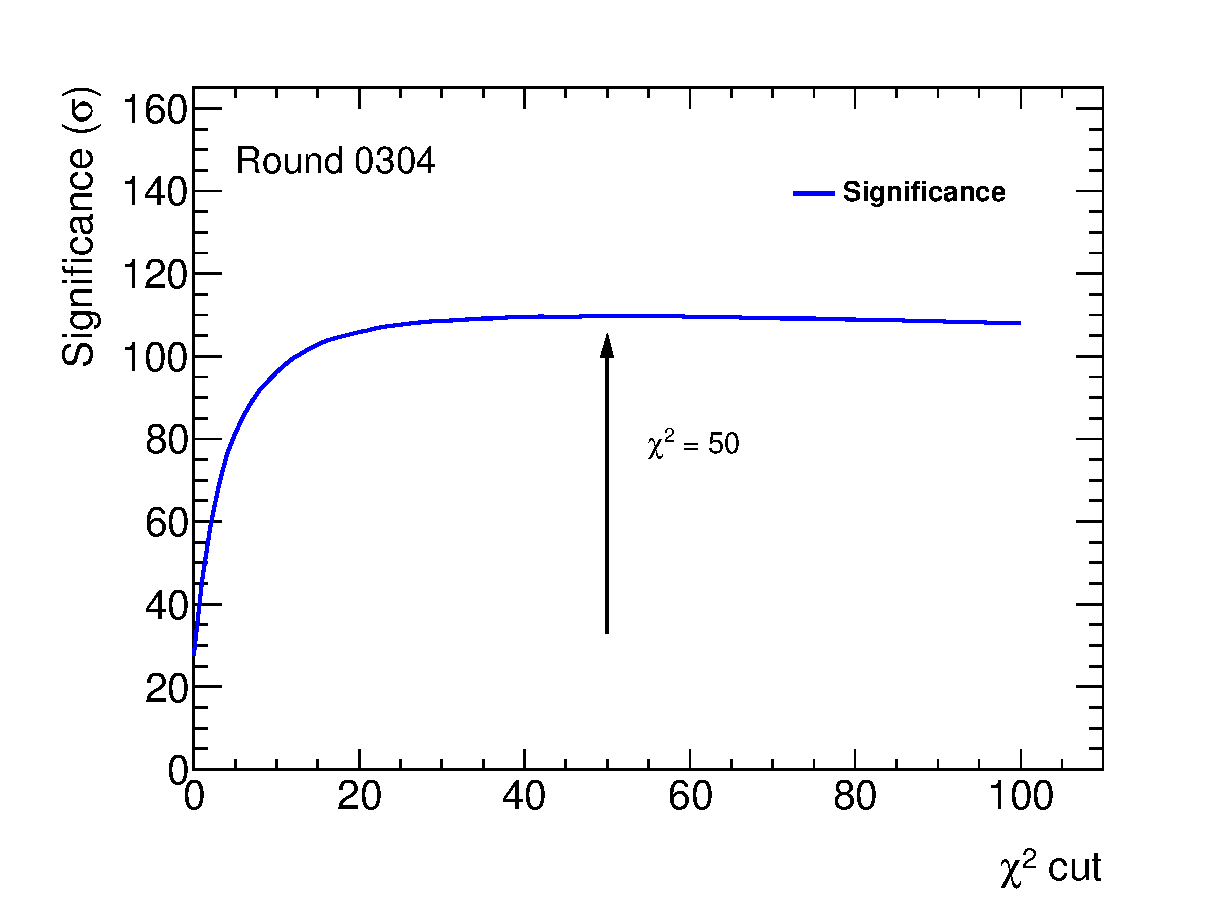
\includegraphics[width=0.40\textwidth]{fig/OptimizeChisq4C_scan_round0304.eps}
        \label{fig:optimize_chisq_scan_round0304}
    }
    \hfill
    \subfloat[Round 15]{
        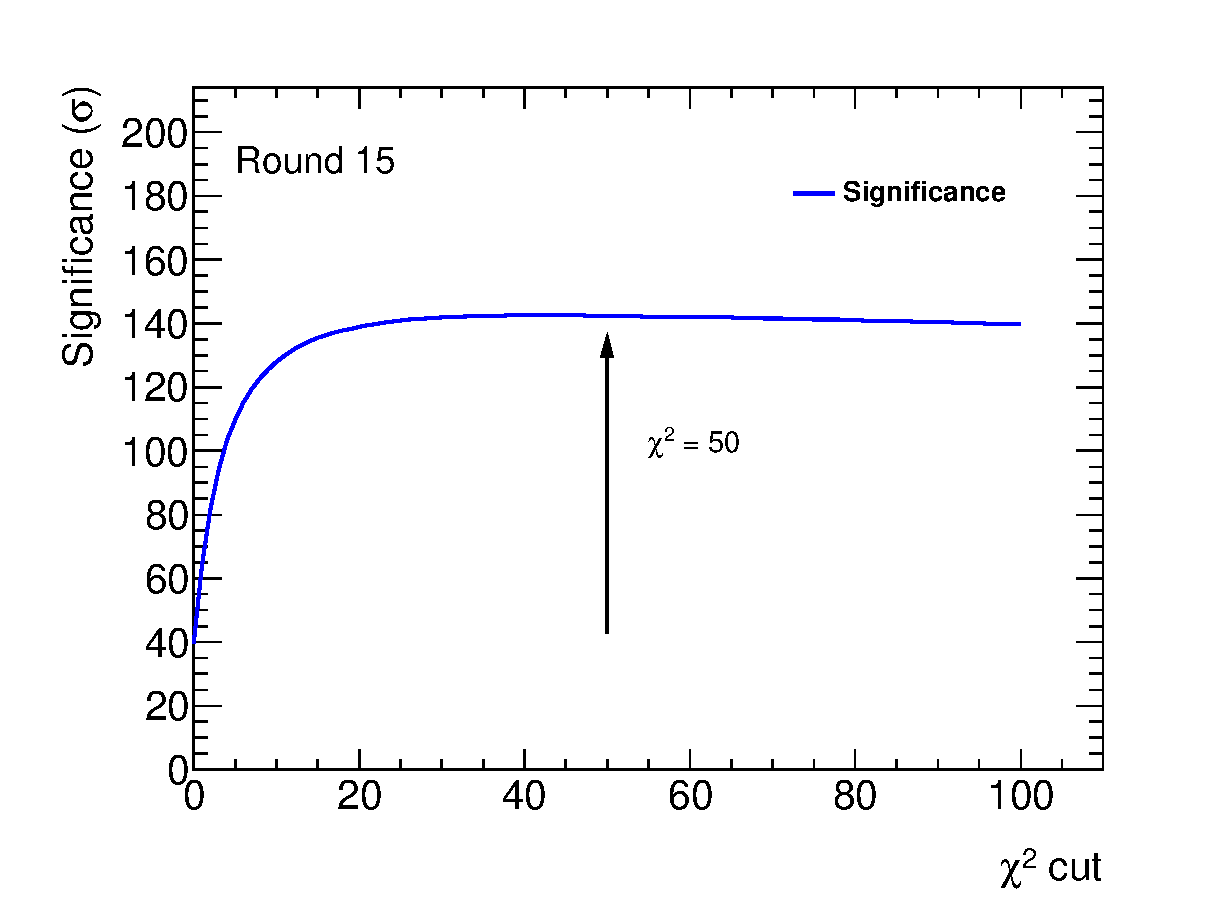
\includegraphics[width=0.40\textwidth]{fig/OptimizeChisq4C_scan_round15.eps}
        \label{fig:optimize_chisq_scan_round15}
    }
    \hfill
    \subfloat[Round 17]{
        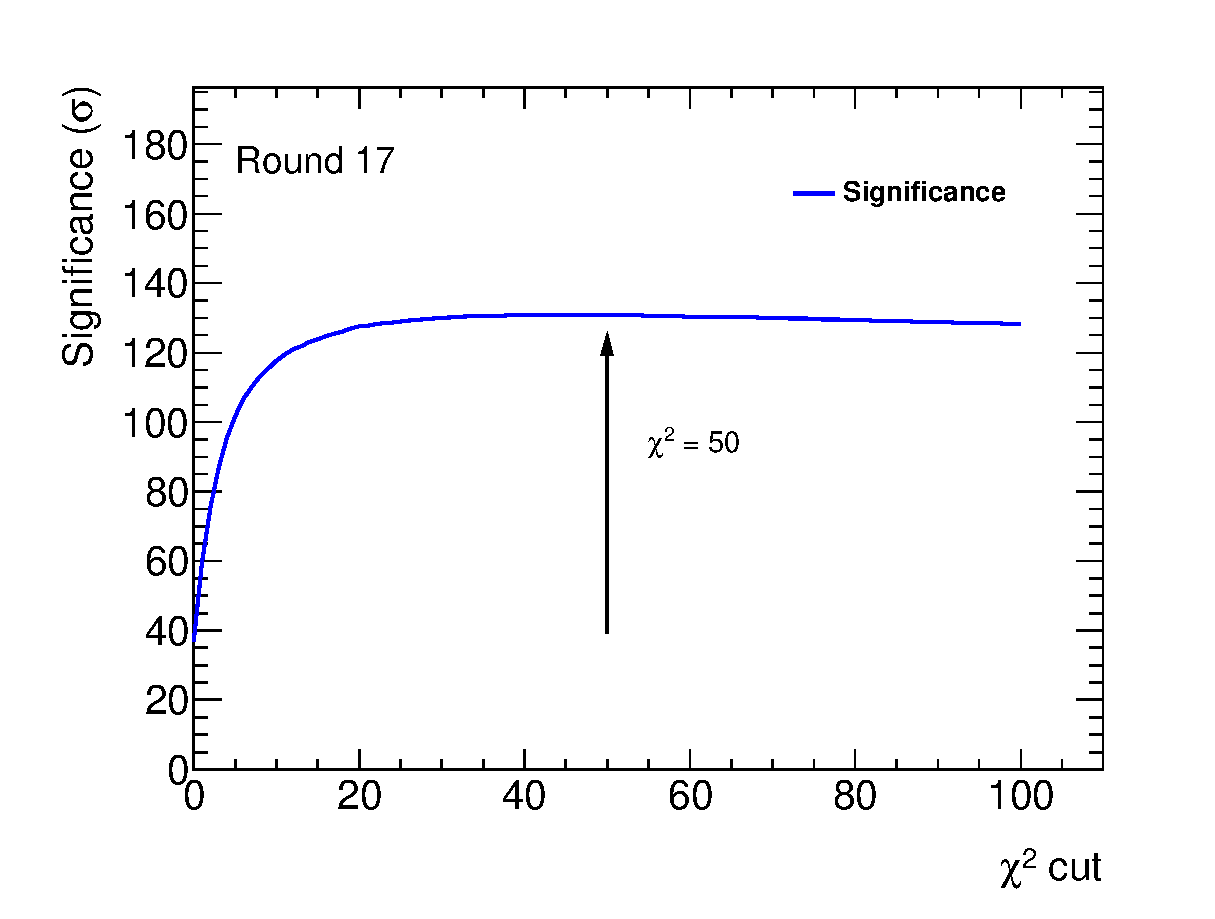
\includegraphics[width=0.40\textwidth]{fig/OptimizeChisq4C_scan_round17.eps}
        \label{fig:optimize_chisq_scan_round17}
    }
    \caption{FOM ($S/\sqrt{S+B}$) as a function of the applied $\chi^2$ cut value for (a) Round~03/04, (b) Round~15, and (c) Round~17 data samples.}
    \label{fig:chisq_optimization_rounds}
\end{figure}

Based on the optimal $\chi^2_{\mathrm{KF}}$ selection, the invariant mass
spectrum of the $3\pi$ system ($M_{3\pi}$) can be divided into three distinct
regions for further study: the $\omega(782)$ region, the $\phi(1020)$ region,
and a higher-mass region associated with possible
$\omega^{\prime}/\omega^{\prime\prime}$ excitations. In the high-mass
$\omega^{\prime}/\omega^{\prime\prime}$ region, a significant background
component from events containing additional $\pi^0$ mesons was observed. To
quantify this, the number of $\pi^0$ candidates per event was counted, where
any $\pi^0$ candidate satisfying a one-constraint kinematic fit $\chi^2 < 200$
was accepted. The distribution of this $\pi^0$ multiplicity is shown in
Fig.~\ref{fig:pi0_multiplicity}. To suppress this specific background, a
requirement of exactly one $\pi^0$ candidate per event was applied exclusively
in the $\omega^{\prime}/\omega^{\prime\prime}$ mass region. No such restriction
was applied to the $\omega(782)$ and $\phi(1020)$ signal regions. The following
studies and distributions are based on the Round~16 data sample.

\begin{figure}[htbp]
    \centering
    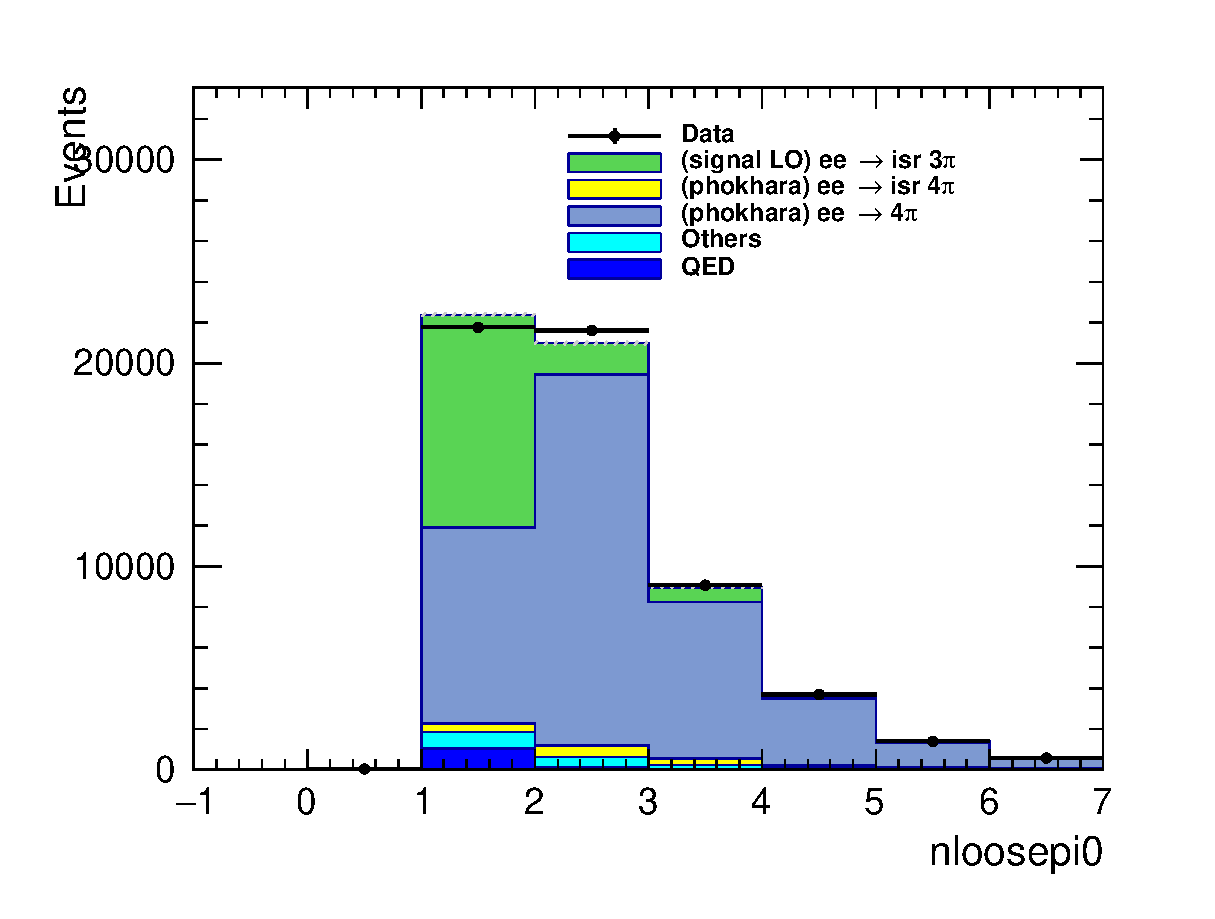
\includegraphics[width=0.45\textwidth]{fig/nloosepi0_origin.eps}
    \caption{Distribution of the number of $\pi^0$ candidates per event in the $\omega^{\prime}/\omega^{\prime\prime}$ mass region using the Round~16 data. A $\pi^0$ candidate is counted if its 1C kinematic fit $\chi^2 < 200$.}
    \label{fig:pi0_multiplicity}
\end{figure}

The resulting $M_{3\pi}$ invariant mass spectra, after applying all selection
criteria including the region-specific $\pi^0$ multiplicity cut, are presented
separately for the three mass regions in
Fig.~\ref{fig:all_rounds_3pi}. The $e^{+}e^{-} \to
    \pi^{+}\pi^{-}\pi^{0}\pi^{0}\gamma_{\text{ISR}}$ contribution is negligible and
will not be treated as a separate background in the subsequent fitting
procedure; only the non-ISR $e^{+}e^{-} \to \pi^{+}\pi^{-}\pi^{0}\pi^{0}$
process will be explicitly estimated using data-driven methods and constrained
in the fit.
\begin{figure}[htbp]
\centering

% === Row 1: Round 03/04 ===
\subfloat[Round 03/04, $\omega(782)$]{
    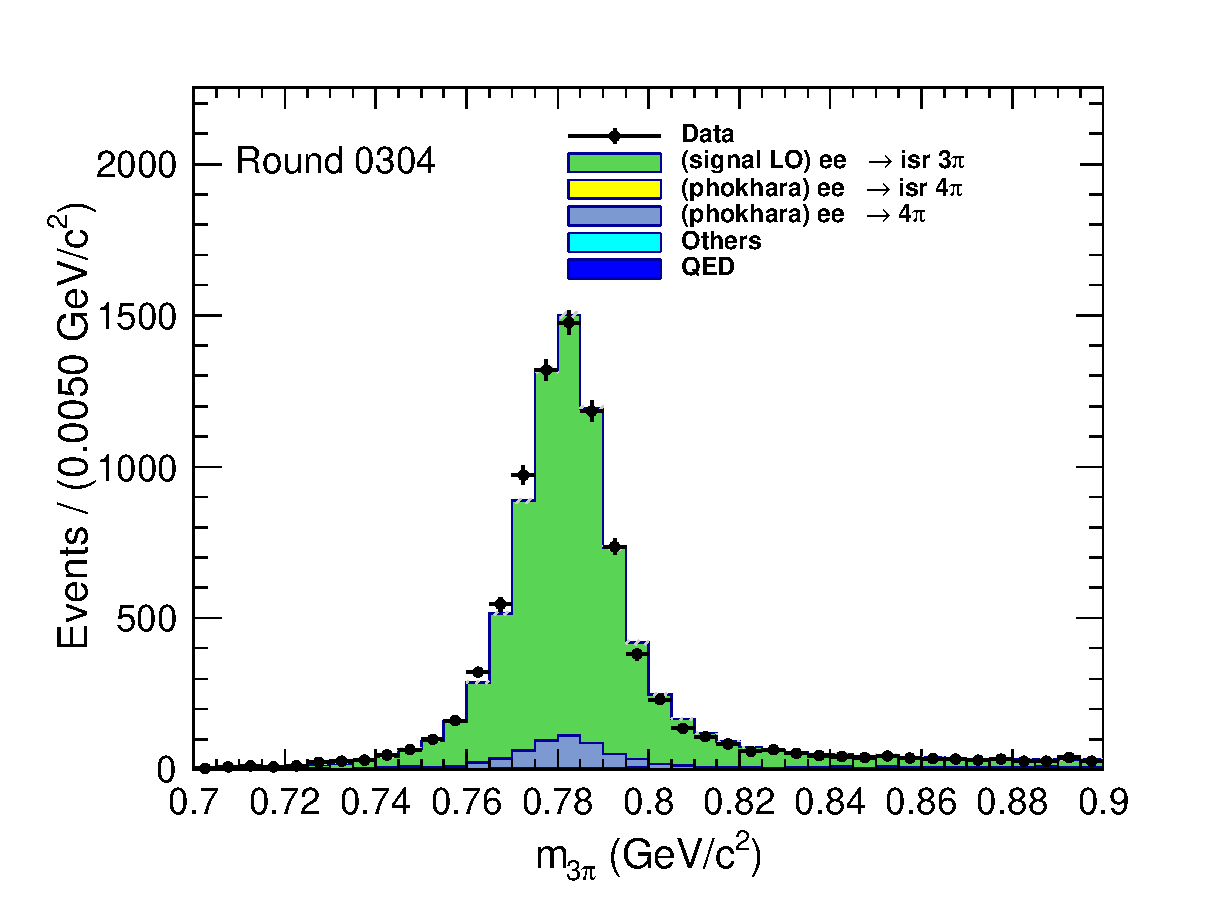
\includegraphics[width=0.32\textwidth]{fig/round0304_omega.eps}
    \label{fig:r0304_omega}
}\hfill
\subfloat[Round 03/04, $\phi(1020)$]{
    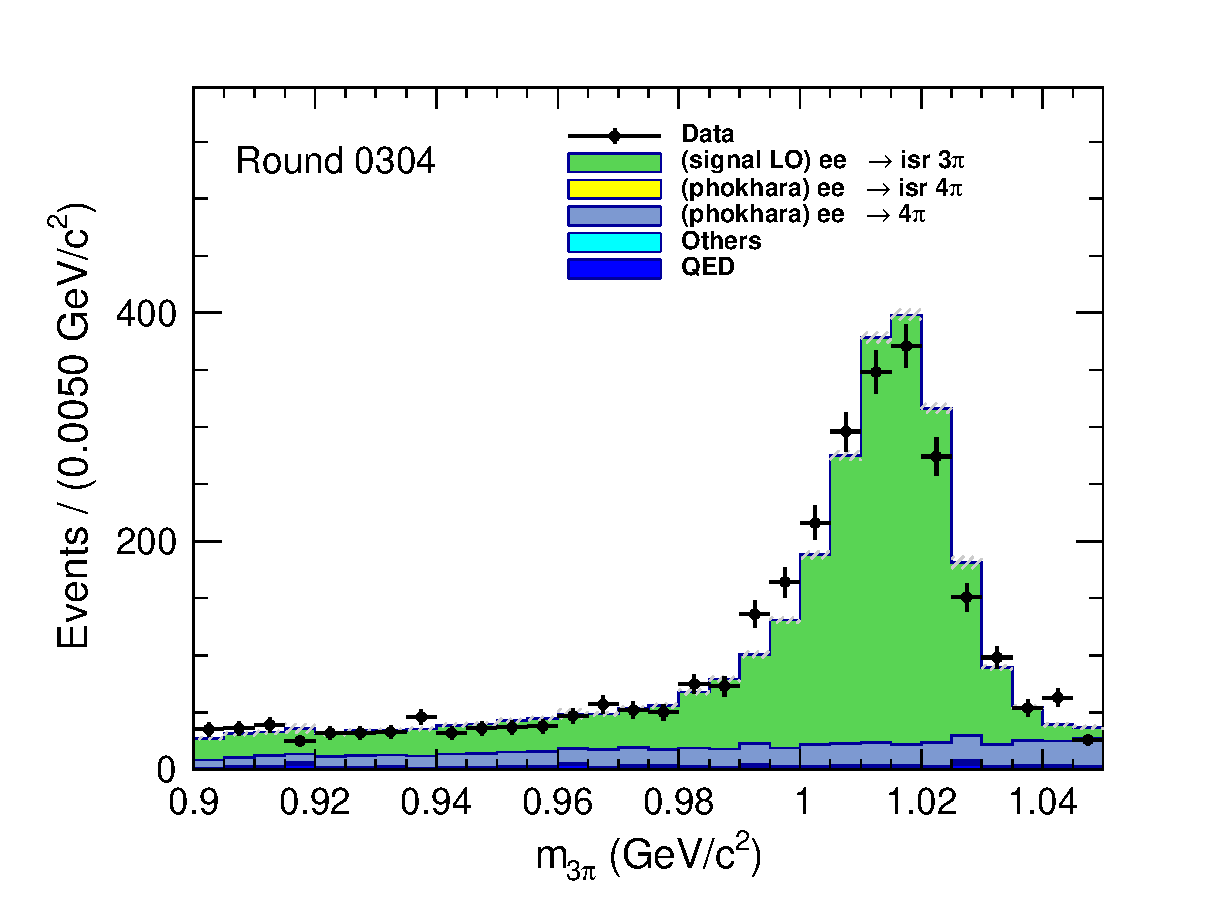
\includegraphics[width=0.32\textwidth]{fig/round0304_phi.eps}
    \label{fig:r0304_phi}
}\hfill
\subfloat[Round 03/04, $\omega^{\prime}/\omega^{\prime\prime}$]{
    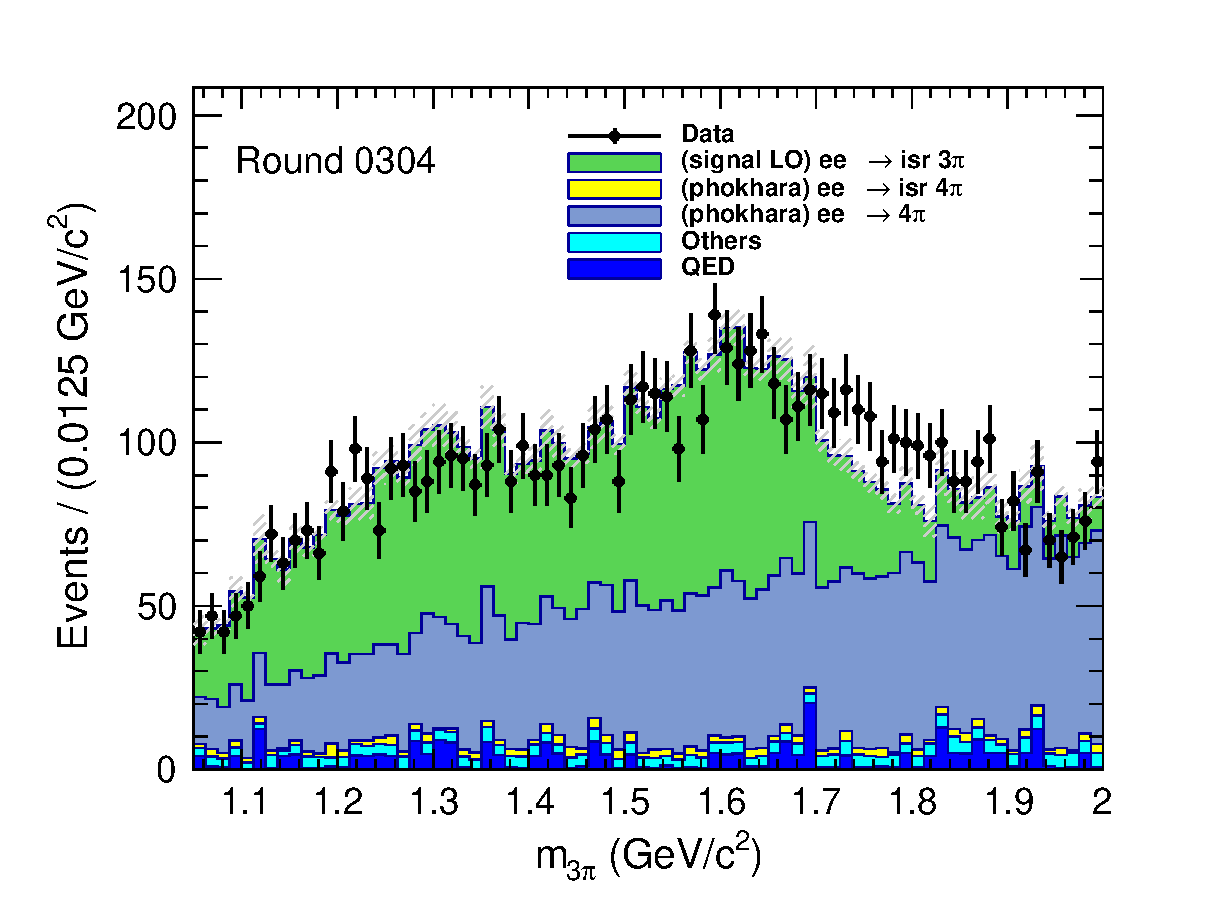
\includegraphics[width=0.32\textwidth]{fig/round0304_omegaprime.eps}
    \label{fig:r0304_omegaprime}
}

% \vspace{0.5\baselineskip}

% === Row 2: Round 15 ===
\subfloat[Round 15, $\omega(782)$]{
    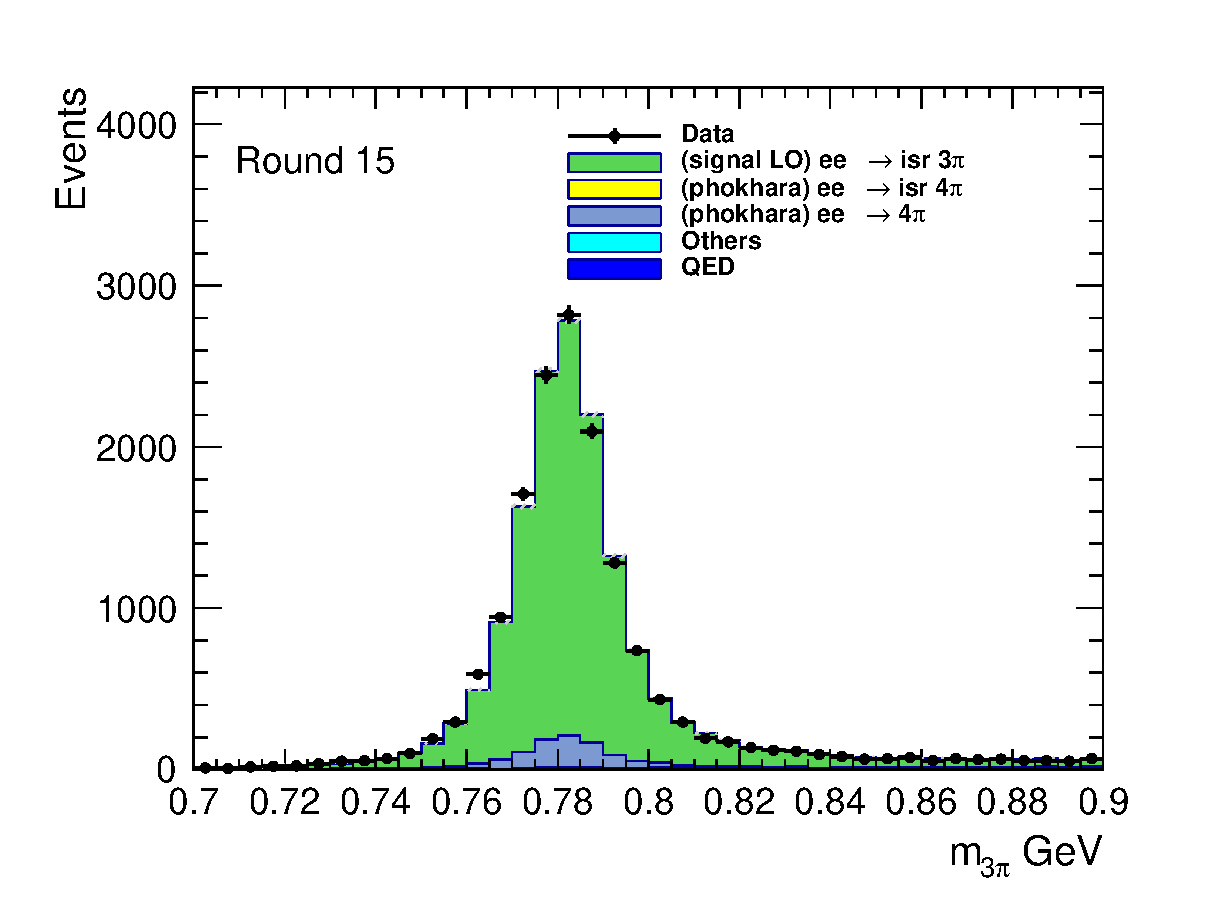
\includegraphics[width=0.32\textwidth]{fig/round15_omega.eps}
    \label{fig:r15_omega}
}\hfill
\subfloat[Round 15, $\phi(1020)$]{
    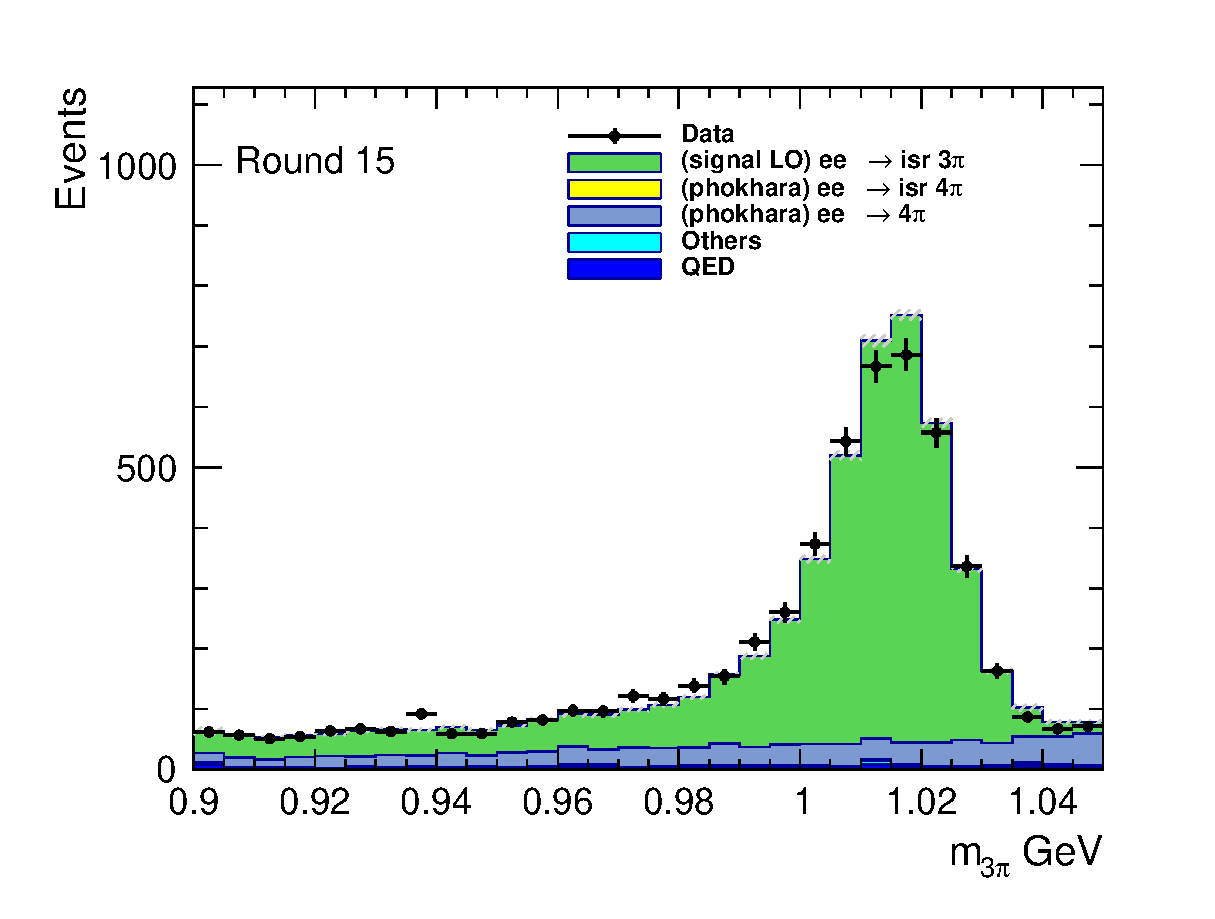
\includegraphics[width=0.32\textwidth]{fig/round15_phi.eps}
    \label{fig:r15_phi}
}\hfill
\subfloat[Round 15, $\omega^{\prime}/\omega^{\prime\prime}$]{
    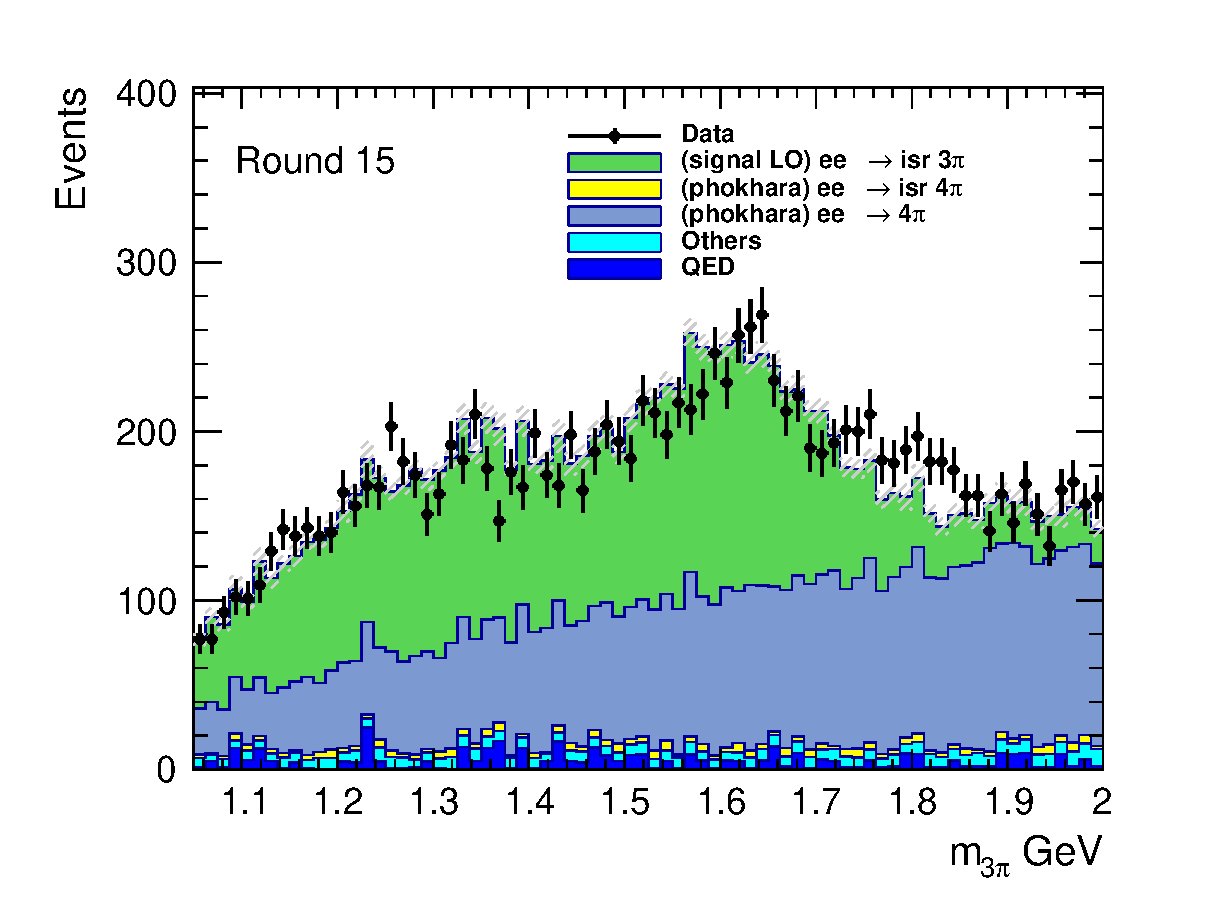
\includegraphics[width=0.32\textwidth]{fig/round15_omegaprime.eps}
    \label{fig:r15_omegaprime}
}

% \vspace{0.5\baselineskip}

% === Row 3: Round 16 ===
\subfloat[Round 16, $\omega(782)$]{
    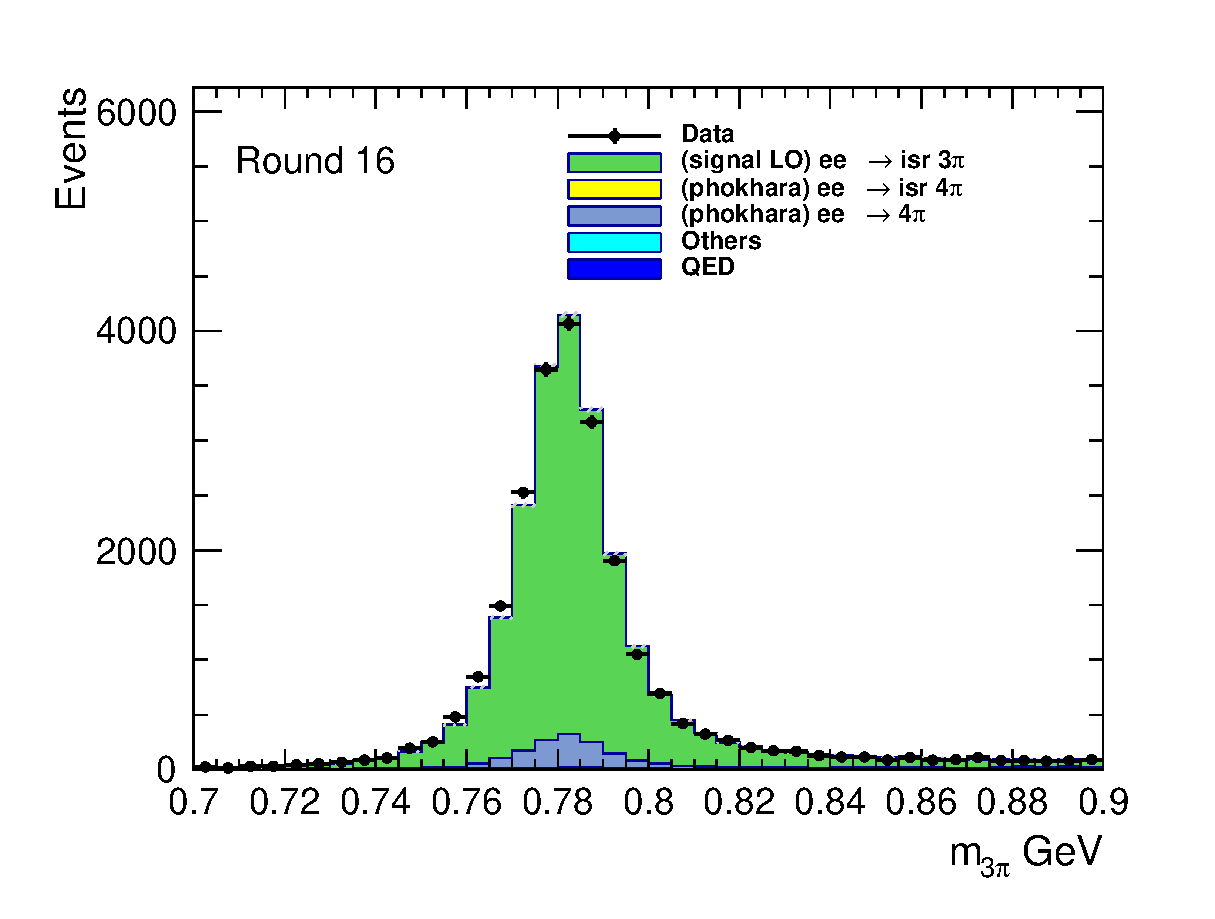
\includegraphics[width=0.32\textwidth]{fig/round16_omega.eps}
    \label{fig:r16_omega}
}\hfill
\subfloat[Round 16, $\phi(1020)$]{
    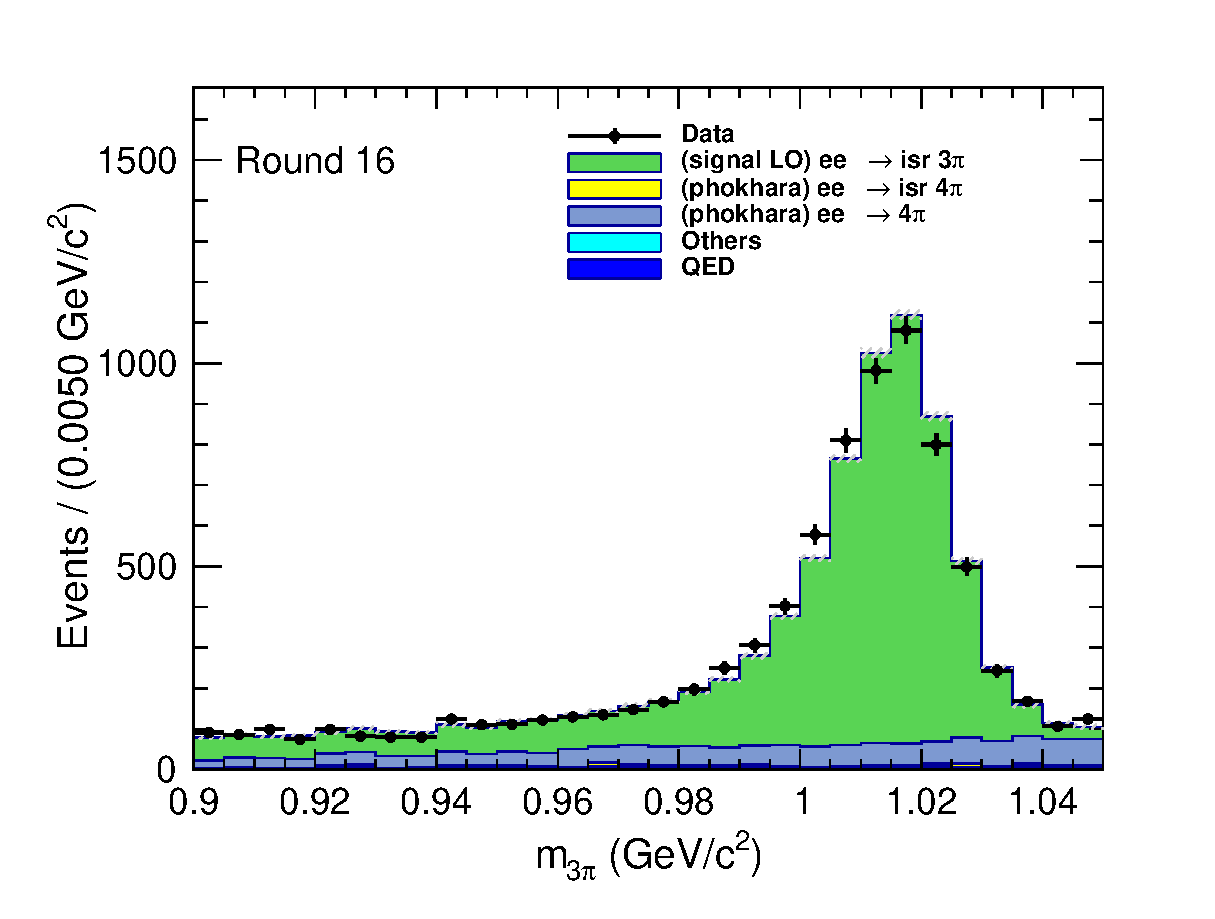
\includegraphics[width=0.32\textwidth]{fig/round16_phi.eps}
    \label{fig:r16_phi}
}\hfill
\subfloat[Round 16, $\omega^{\prime}/\omega^{\prime\prime}$]{
    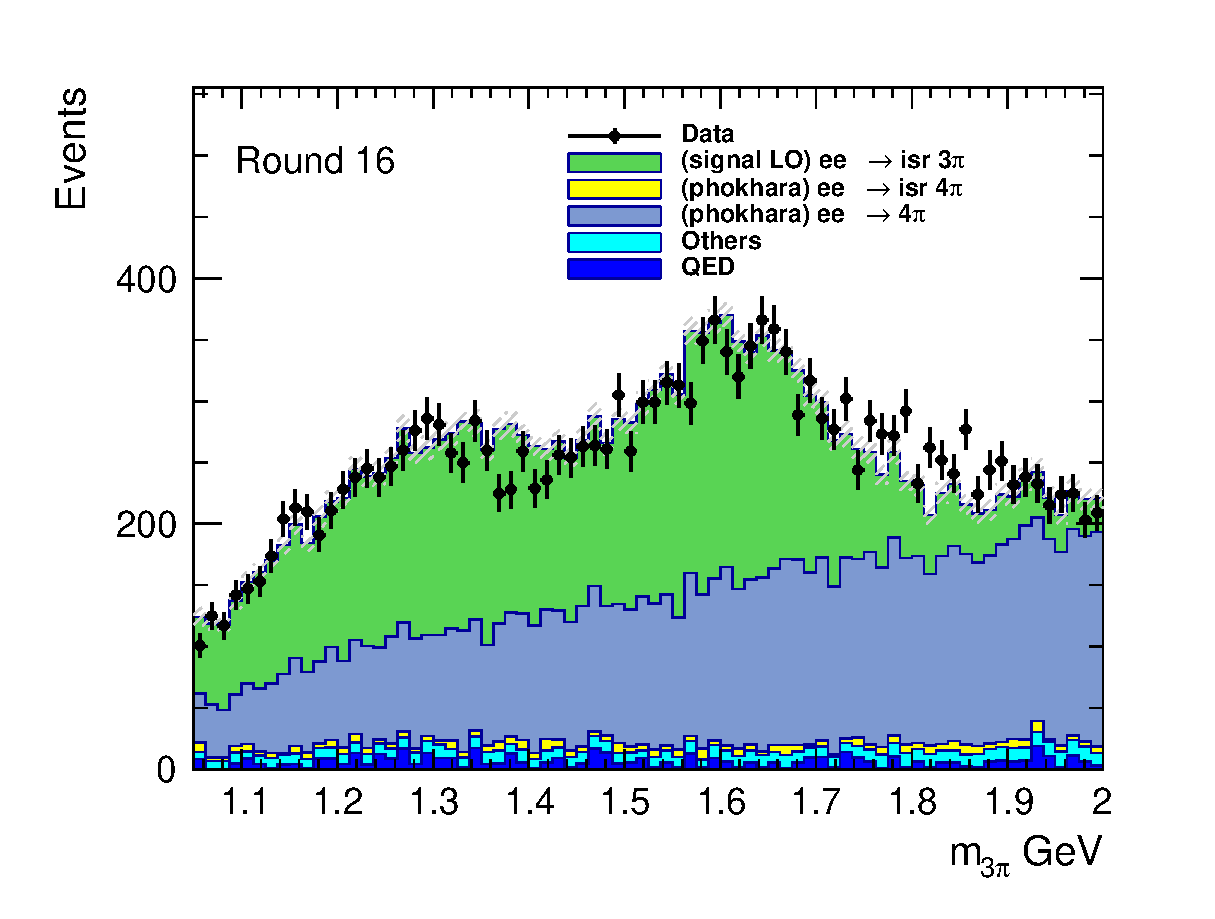
\includegraphics[width=0.32\textwidth]{fig/round16_omegaprime.eps}
    \label{fig:r16_omegaprime}
}

% \vspace{0.5\baselineskip}

% === Row 4: Round 17 ===
\subfloat[Round 17, $\omega(782)$]{
    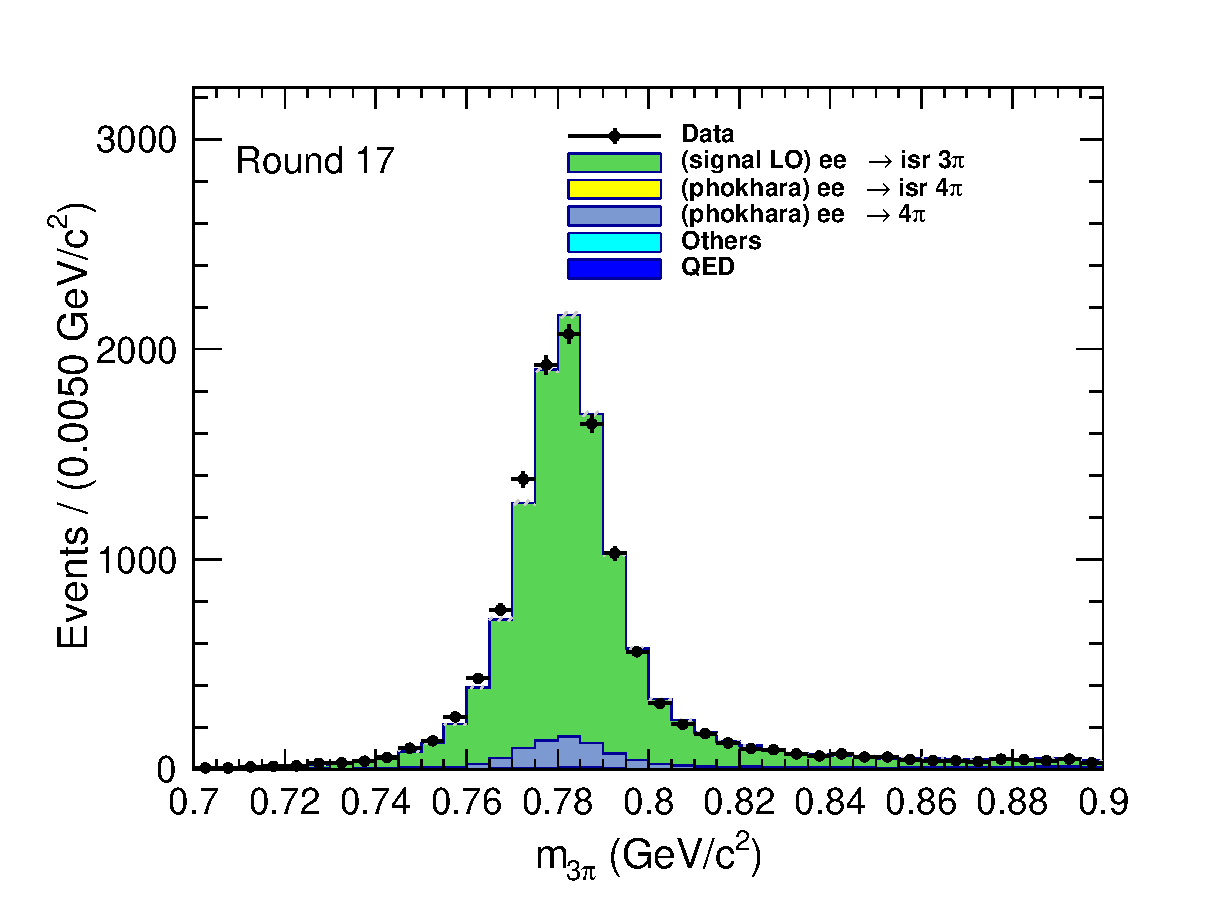
\includegraphics[width=0.32\textwidth]{fig/round17_omega.eps}
    \label{fig:r17_omega}
}\hfill
\subfloat[Round 17, $\phi(1020)$]{
    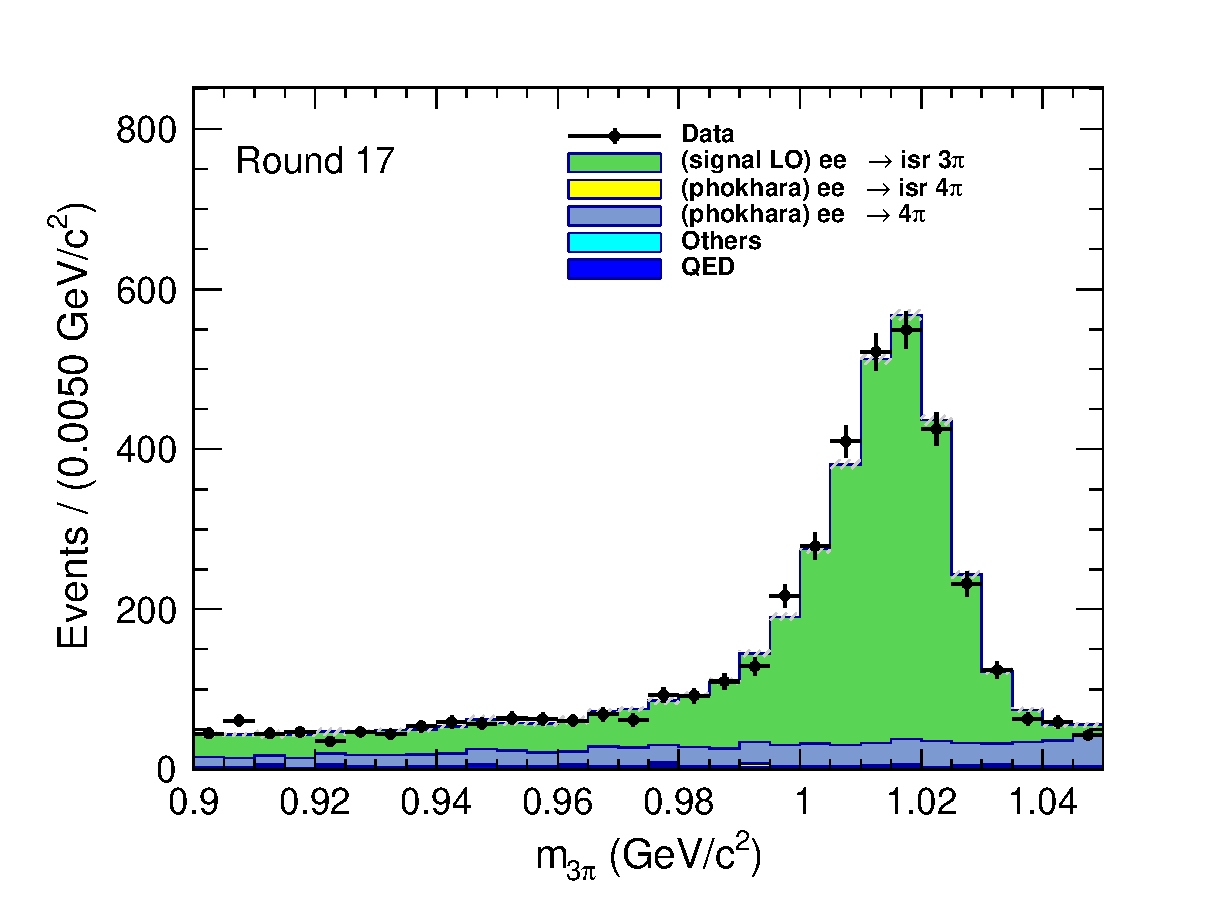
\includegraphics[width=0.32\textwidth]{fig/round17_phi.eps}
    \label{fig:r17_phi}
}\hfill
\subfloat[Round 17, $\omega^{\prime}/\omega^{\prime\prime}$]{
    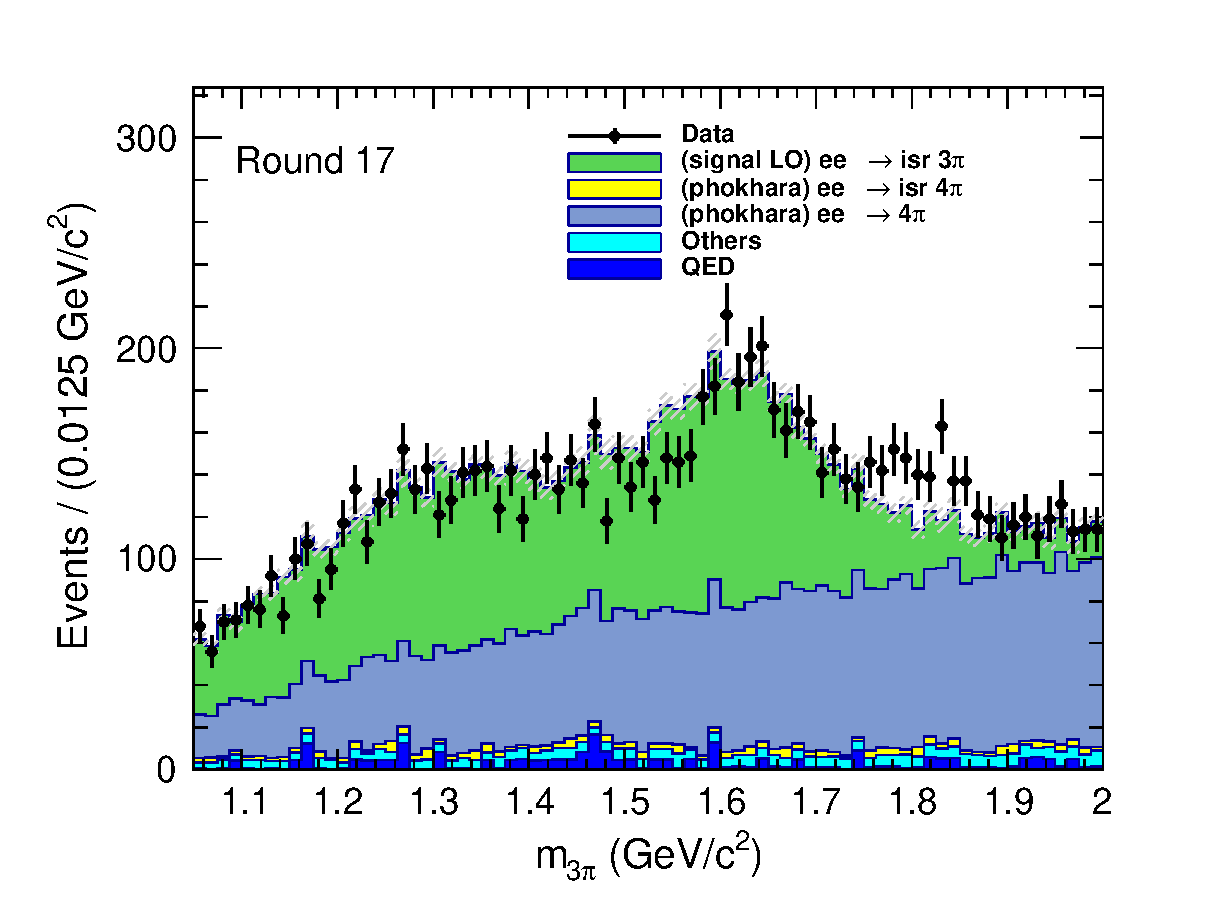
\includegraphics[width=0.32\textwidth]{fig/round17_omegaprime.eps}
    \label{fig:r17_omegaprime}
}

\caption{Invariant mass spectra $M_{3\pi}$ for different data rounds and mass regions with $N_{\pi^0}=1$ (other columns no $\pi^0$ multiplicity cut).}
\label{fig:all_rounds_3pi}
\end{figure}
% The $3\pi$ invariant mass distribution obtained with the $\chi^{2}_{\mathrm{KF}} < 50$ selection is presented in Fig.~\ref{fig:mass3pi_stacked}. This plot, using the Round~16 data sample, displays the data in comparison with the stacked MC predictions for the signal and background components.

% \begin{figure}[htbp]
%     \centering
%     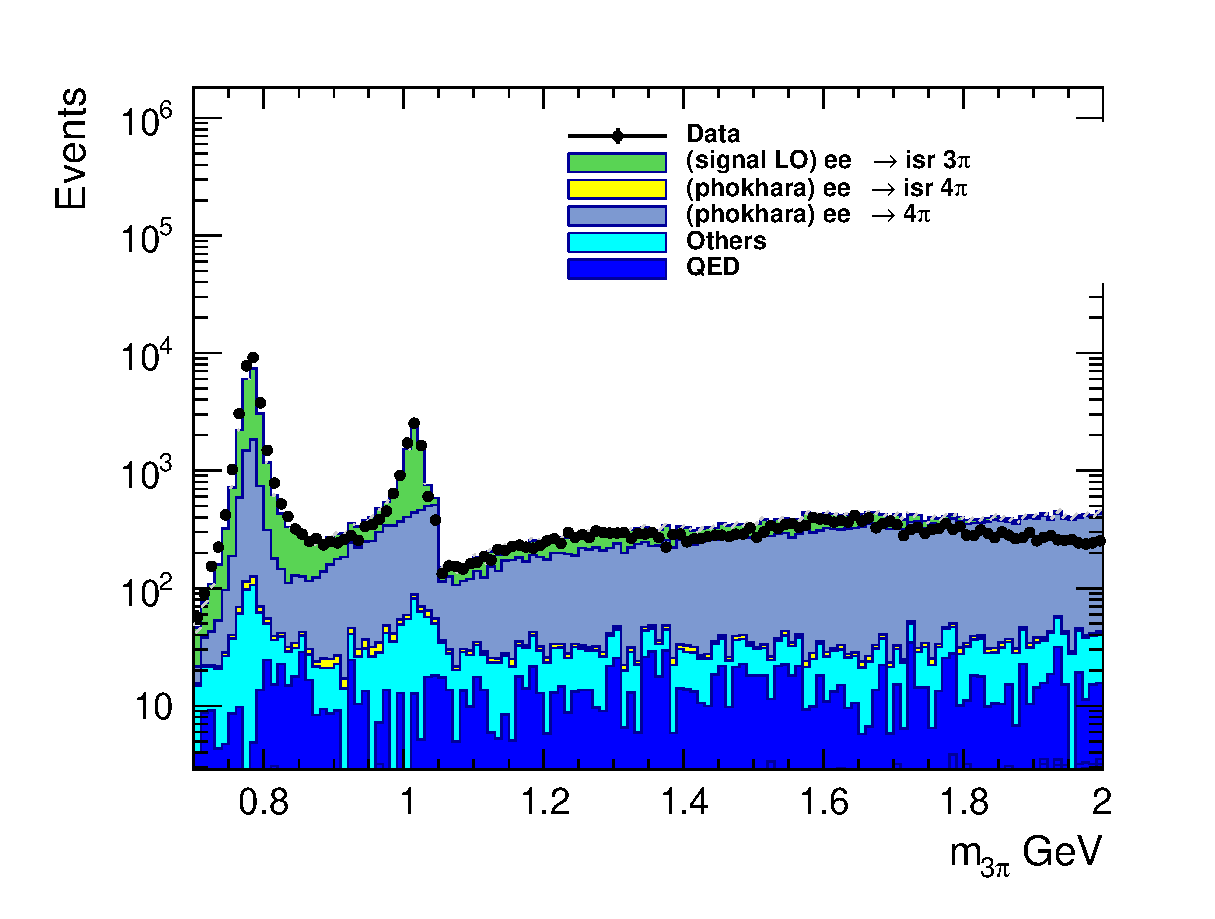
\includegraphics[width=0.6\textwidth]{fig/mass3pi.eps}
%     \caption{The $3\pi$ invariant mass distribution after applying the $\chi^{2}_{\mathrm{KF}} < 50$ selection to the Round~16 data sample. The stacked histogram shows the contributions from the signal process $e^{+}e^{-} \to \pi^{+}\pi^{-}\pi^{0}$ and various background processes, including the dominant $e^{+}e^{-} \to \pi^{+}\pi^{-}\pi^{0}\pi^{0}$ and $e^{+}e^{-} \to \pi^{+}\pi^{-}\pi^{0}\pi^{0}\gamma_{\text{ISR}}$ backgrounds.}
%     \label{fig:mass3pi_stacked}
% \end{figure}

\clearpage
\subsection{Estimate of $\ee\to\pip\pim\piz\piz$}
In estimating the $e^{+}e^{-} \to \pi^{+}\pi^{-}\pi^{0}\pi^{0}$ background, the
following strategy was adopted:

It is assumed that the total yield of $e^{+}e^{-} \to
    \pi^{+}\pi^{-}\pi^{0}\pi^{0}$ events produced in the data is a fixed quantity.
This process enters our signal region primarily when a photon from one of the
$\pi^{0}$ decays is misidentified as an initial-state radiation photon
($\gamma_{\text{ISR}}$). Consequently, two distinct selection efficiencies can
be calculated: $\epsilon_{\text{sig}}$ (the efficiency for $e^{+}e^{-} \to
    \pi^{+}\pi^{-}\pi^{0}\pi^{0}$ events to be selected as signal candidates) and
$\epsilon_{\text{bkg}}$ (the efficiency for the same process to enter the
$3\pi$ signal region as background).

When $e^{+}e^{-} \to \pi^{+}\pi^{-}\pi^{0}\pi^{0}$ events are selected as
signal, the same analysis procedure as for the signal is applied to construct
the $3\pi$ invariant mass spectrum, thereby obtaining the distribution of this
process in data. Using the ratio of these two efficiencies, $R =
    \epsilon_{\text{bkg}} / \epsilon_{\text{sig}}$, the observed $e^{+}e^{-} \to
    \pi^{+}\pi^{-}\pi^{0}\pi^{0}$ signal distribution can be converted into an
estimate of its background distribution in the signal region. Specifically:
\begin{equation}
    N_{\text{bkg}} = R \times N_{\text{sig}}^{\text{obs}} = \frac{\epsilon_{\text{bkg}}}{\epsilon_{\text{sig}}} \times N_{\text{sig}}^{\text{obs}},
\end{equation}
where $N_{\text{sig}}^{\text{obs}}$ is the number of observed $e^{+}e^{-} \to
    \pi^{+}\pi^{-}\pi^{0}\pi^{0}$ signal events in data, and $N_{\text{bkg}}$ is
the estimated number of background events from this process in the signal
region.

This method provides a data-driven conversion from the observed signal
distribution to the background distribution through efficiency correction.

When treating $e^{+}e^{-} \to \pi^{+}\pi^{-}\pi^{0}\pi^{0}$ as the signal, the
selection criteria are designed such that the same event sample also satisfies
a loose selection for $e^{+}e^{-} \to
    \gamma_{\mathrm{ISR}}\pi^{+}\pi^{-}\pi^{0}$. This ensures that the invariant
mass of the three-pion system is automatically defined within the latter
process.

The combined selection proceeds as follows: events are required to meet the
criteria for both processes. The first step applies the full $e^{+}e^{-} \to
    \pi^{+}\pi^{-}\pi^{0}\pi^{0}$ selection:
\begin{itemize}
    \item \textbf{$\pi^{+}\pi^{-}\pi^{0}\pi^{0}$ Candidate Selection:}
          \begin{itemize}
              \item Exactly two good charged tracks.
              \item $\text{nPi0} \geq 2$ \& \& $\text{nGoodShowers} \geq 4$ (ensuring at least two $\pi^{0}$s).
              \item Application of a total 4-momentum constraint to the initial $e^{+}e^{-}$
                    collision (4C kinematic fit).
              \item The candidate with the minimum $\chi_{\mathrm{4C}}^2$ is chosen.
              \item A requirement of $\chi_{\mathrm{KF}}^{2} < 10$ on the kinematic fit.
          \end{itemize}
\end{itemize}

Subsequently, within the same event, a candidate for $e^{+}e^{-} \to
    \gamma_{\mathrm{ISR}}\pi^{+}\pi^{-}\pi^{0}$ is formed by reinterpreting one of
the $\pi^{0}$s as the $\gamma_{\mathrm{ISR}}$:
\begin{itemize}
    \item \textbf{$\gamma_{\mathrm{ISR}}\pi^{+}\pi^{-}\pi^{0}$ Candidate Selection:}
          \begin{itemize}
              \item The same two good charged tracks.
              \item $\text{nPi0} \geq 1$ \& \& $\text{nGoodShowers} \geq 3$ (ensuring at least one $\pi^{0}$ and one photon assigned as $\gamma_{\mathrm{ISR}}$).
              \item Application of the same total 4-momentum constraint to the initial $e^{+}e^{-}$
                    collision (4C kinematic fit).
              \item The candidate with the minimum $\chi_{\mathrm{4C}}^2$ is chosen.
              \item No additional kinematic fit $\chi^2$ requirement is applied at this stage.
          \end{itemize}
\end{itemize}

This dual-tag strategy guarantees that the reconstructed $3\pi$ system from the
$e^{+}e^{-} \to \gamma_{\mathrm{ISR}}\pi^{+}\pi^{-}\pi^{0}$ hypothesis is
kinematically well-defined, and its invariant mass can be reliably calculated
for the subsequent analysis.

The selection described above results in a highly pure sample of $e^{+}e^{-}
\to \pi^{+}\pi^{-}\pi^{0}\pi^{0}$ events. The invariant mass spectrum of the
corresponding three-pion system from this pure sample, which serves as the
input template for background estimation, is shown in
Fig.~\ref{fig:nonisr4pi_all_rounds_regions}.

\begin{figure}[htbp]
    \centering
    \subfloat[Round 03/04]{
        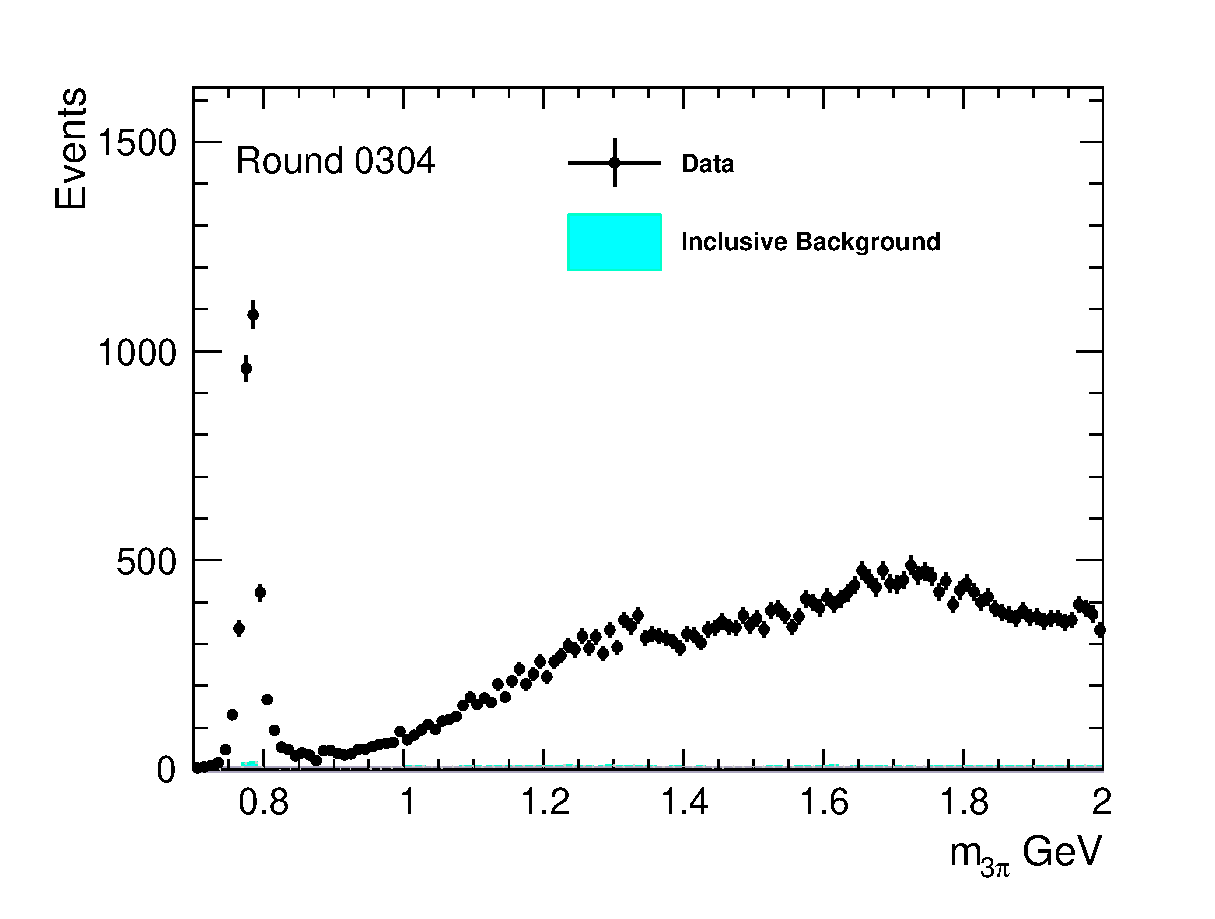
\includegraphics[width=0.40\textwidth]{fig/4pi_3pi_mass_round0304.eps}
        \label{fig:4pi_background_spectrum_round0304}
    }
    \hfill
    \subfloat[Round 15]{
        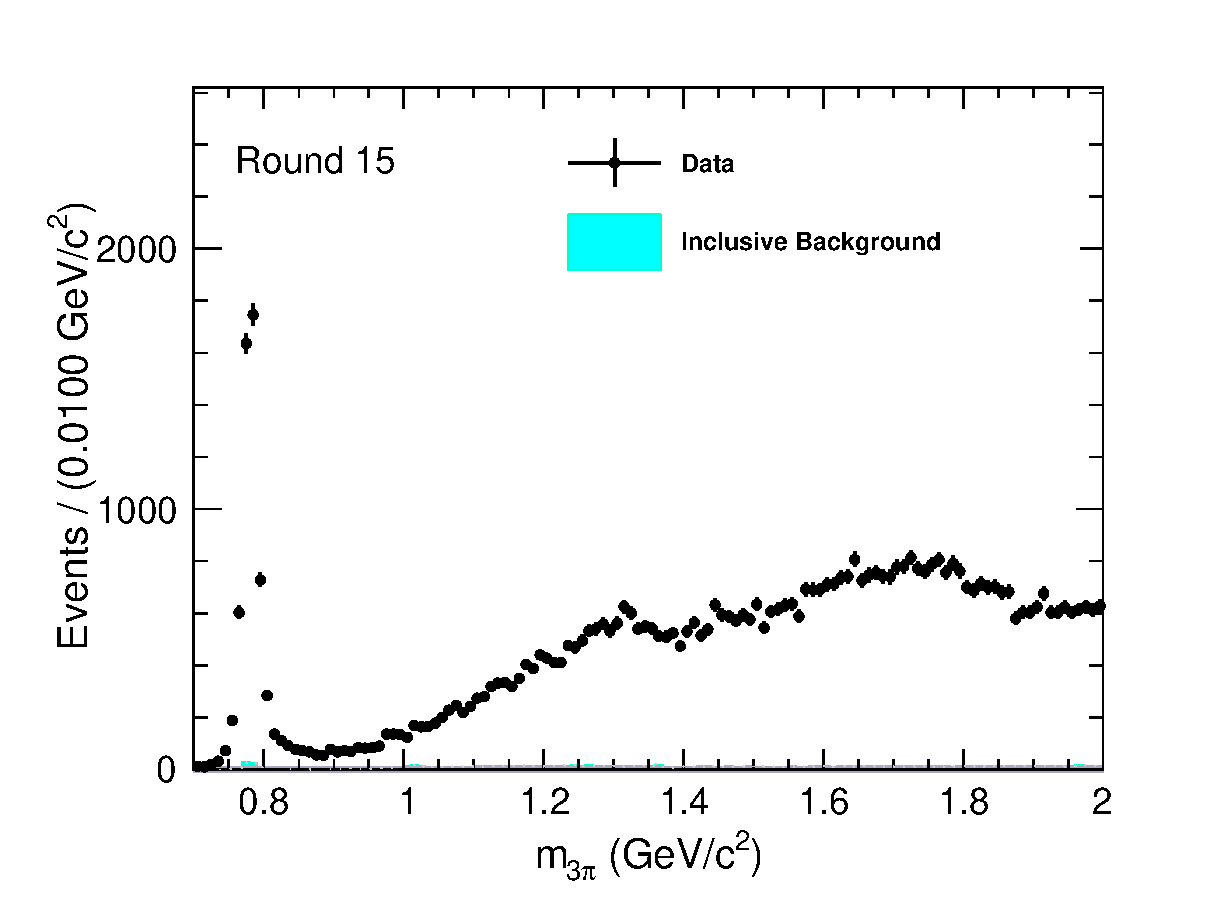
\includegraphics[width=0.40\textwidth]{fig/4pi_3pi_mass_round15.eps}
        \label{fig:4pi_background_spectrum_round15}
    }
    \\
    \subfloat[Round 16]{
        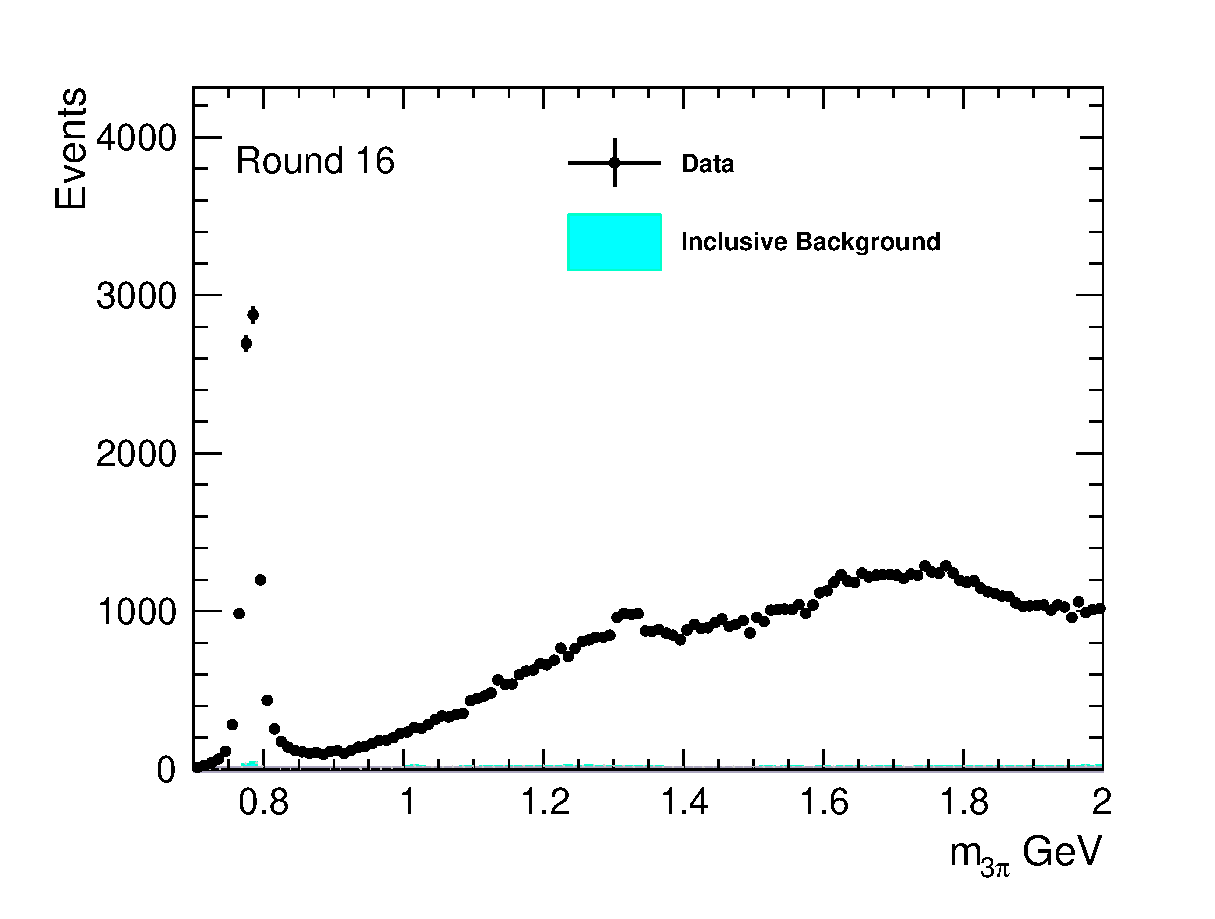
\includegraphics[width=0.40\textwidth]{fig/4pi_3pi_mass_round16.eps}
        \label{fig:4pi_background_spectrum_round16}
    }
    \hfill
    \subfloat[Round 17]{
        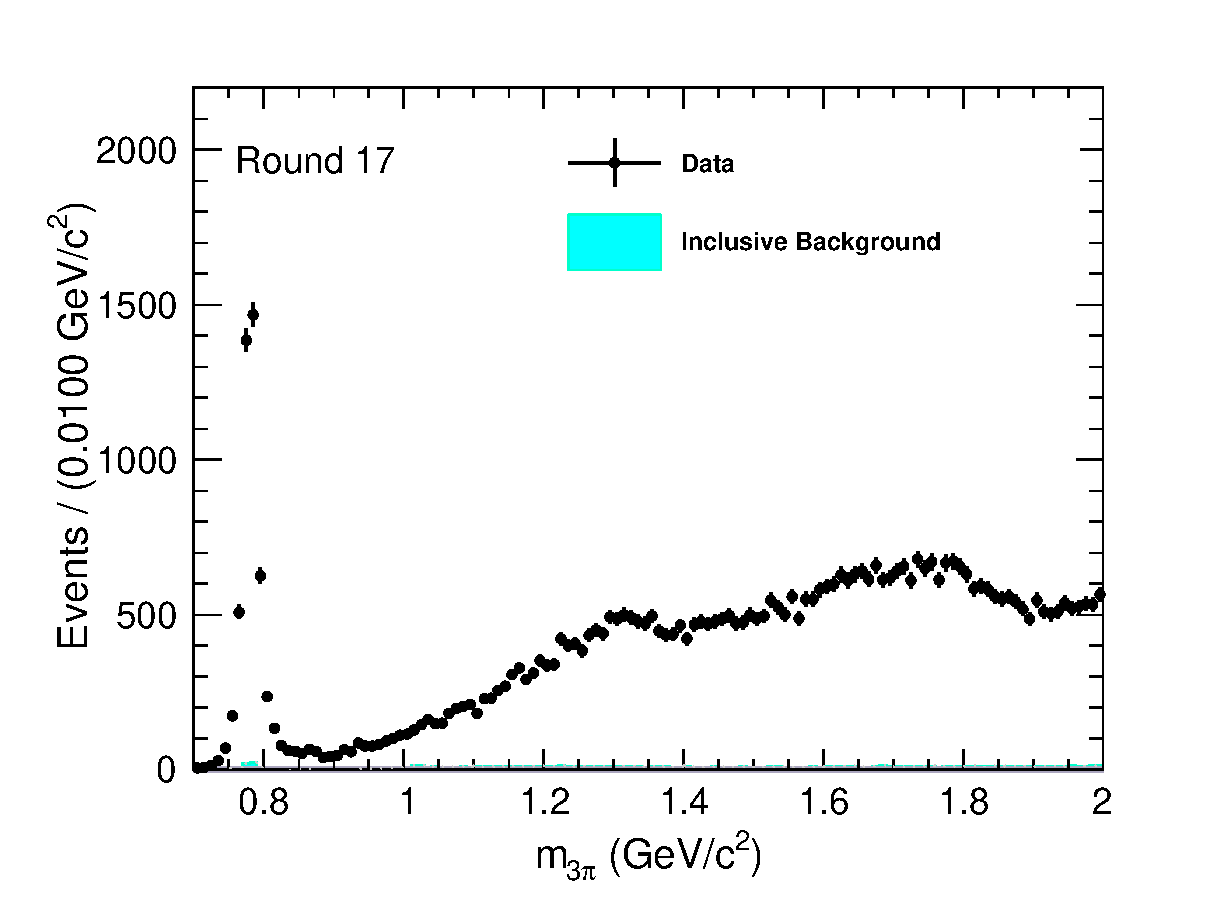
\includegraphics[width=0.40\textwidth]{fig/4pi_3pi_mass_round17.eps}
        \label{fig:4pi_background_spectrum_round17}
    }
    \caption{The $3\pi$ invariant mass spectrum from selected $e^{+}e^{-} \to \pi^{+}\pi^{-}\pi^{0}\pi^{0}$ events in the (a) Round~03/04, (b) Round~15, (c) Round~16, and (d) Round~17 datasets. These distributions, obtained from data after applying the dual-tag selection criteria for $e^{+}e^{-} \to \pi^{+}\pi^{-}\pi^{0}\pi^{0}$, represent the pure signal samples used as templates for background estimation.}
    \label{fig:4pi_background_spectrum}
\end{figure}

The observed distribution in the data, after applying the $e^{+}e^{-} \to
    \pi^{+}\pi^{-}\pi^{0}\pi^{0}$ selection criteria, will be scaled by the
efficiency ratio $R = \epsilon_{\text{bkg}} / \epsilon_{\text{sig}}$ to
estimate the final background contribution of this process in the signal region
of the measurement channel. As established and shown in
Fig.~\ref{fig:4pi_background_spectrum}, the background contamination within
this selected sample is negligible. Therefore, we subtract the inclusive
background histogram from the data histogram in a symbolic manner to obtain the
pure $e^{+}e^{-} \to \pi^{+}\pi^{-}\pi^{0}\pi^{0}$ event yield. The resulting
background-subtracted signal distributions in the three $3\pi$ invariant mass
regions are presented in Fig.~\ref{fig:nonisr4pi_all_rounds_regions}. All other
backgrounds will be subtracted directly.

% 添加结果图（四个物理区域，四个数据周期）
\begin{figure}[htbp]
\centering

% === Row 1: Round 03/04 ===
\subfloat[Round 03/04, $\omega(782)$ region]{
    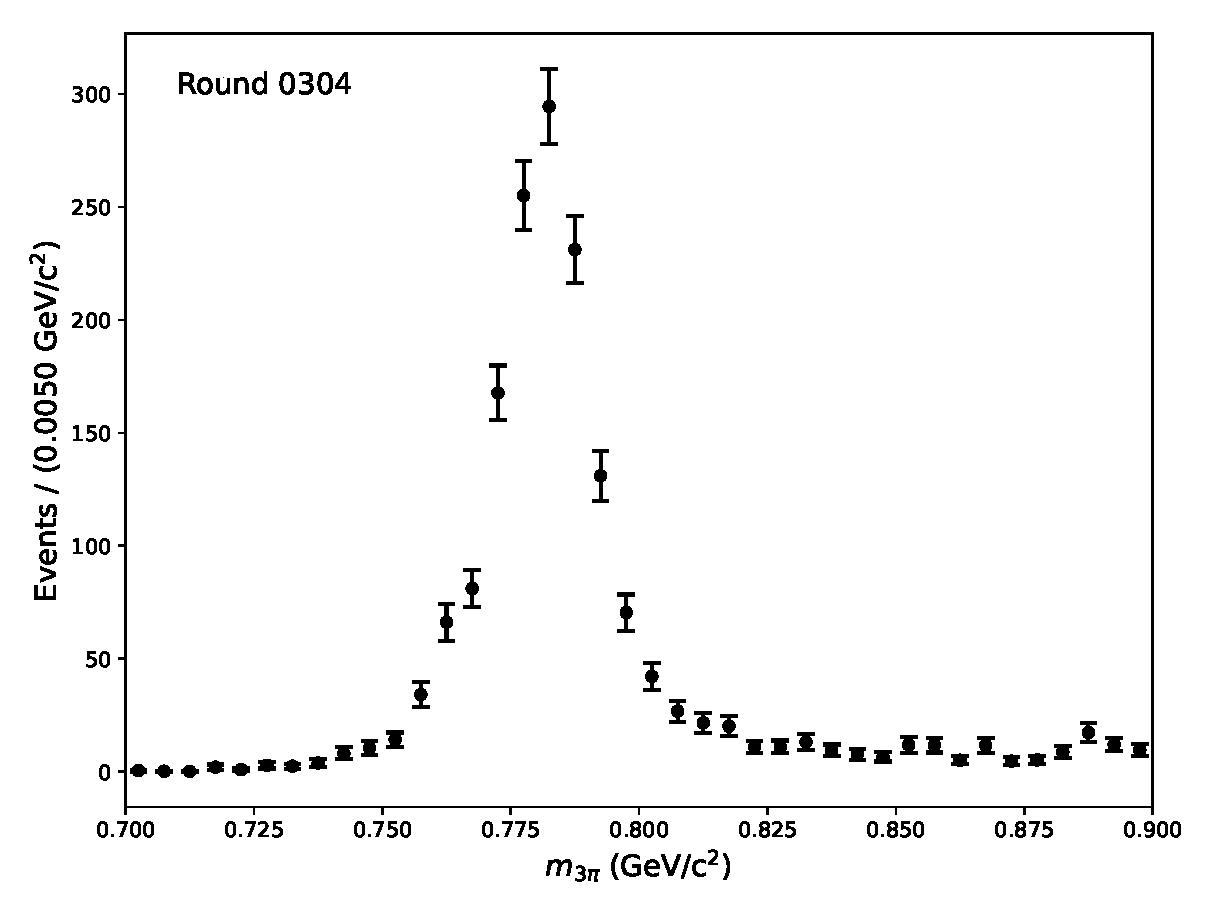
\includegraphics[width=0.32\textwidth]{fig/nonisr4pi_round0304_region1_plot.eps}
    \label{fig:nonisr4pi_r0304_region1}
}\hfill
\subfloat[Round 03/04, $\phi(1020)$ region]{
    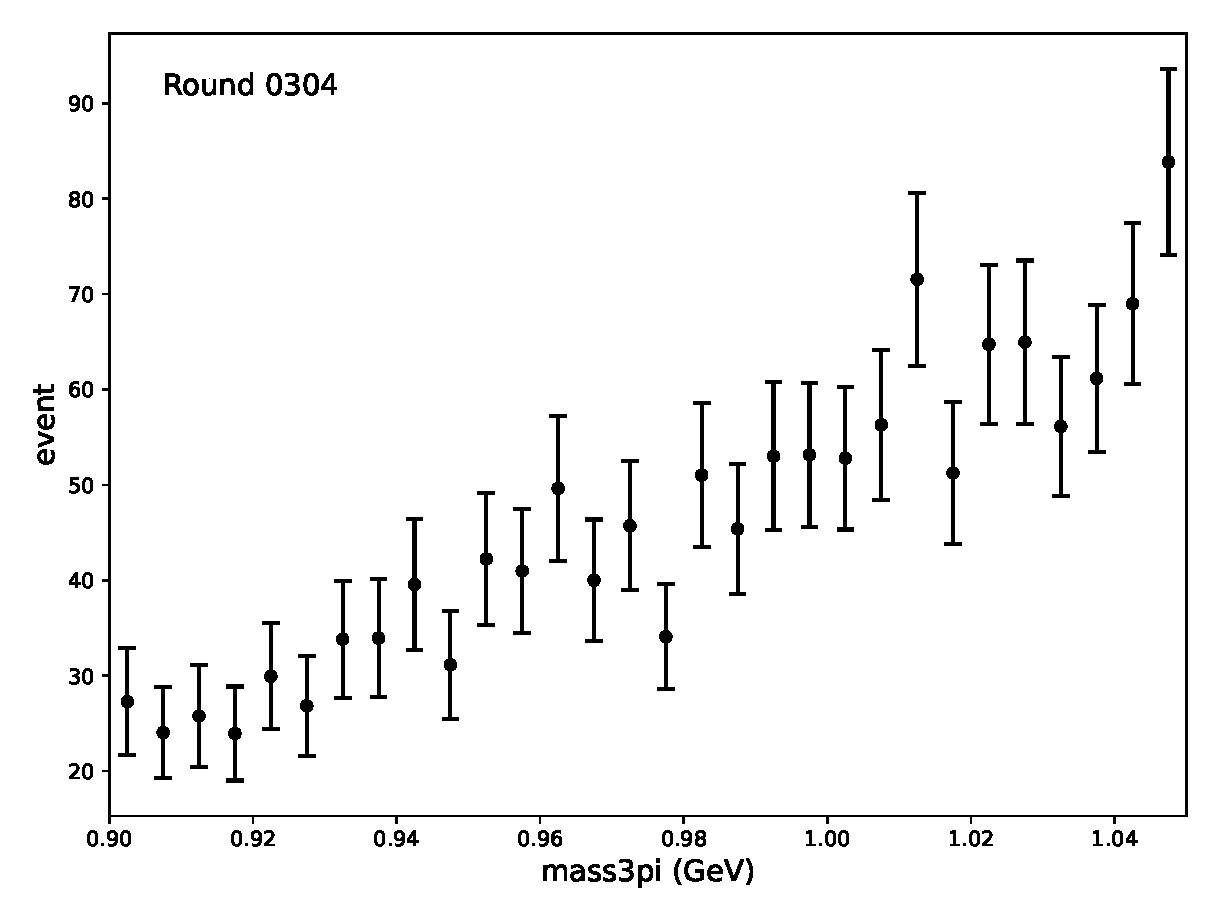
\includegraphics[width=0.32\textwidth]{fig/nonisr4pi_round0304_region2_plot.eps}
    \label{fig:nonisr4pi_r0304_region2}
}\hfill
\subfloat[Round 03/04, $\omega^{\prime}/\omega^{\prime\prime}$ region]{
    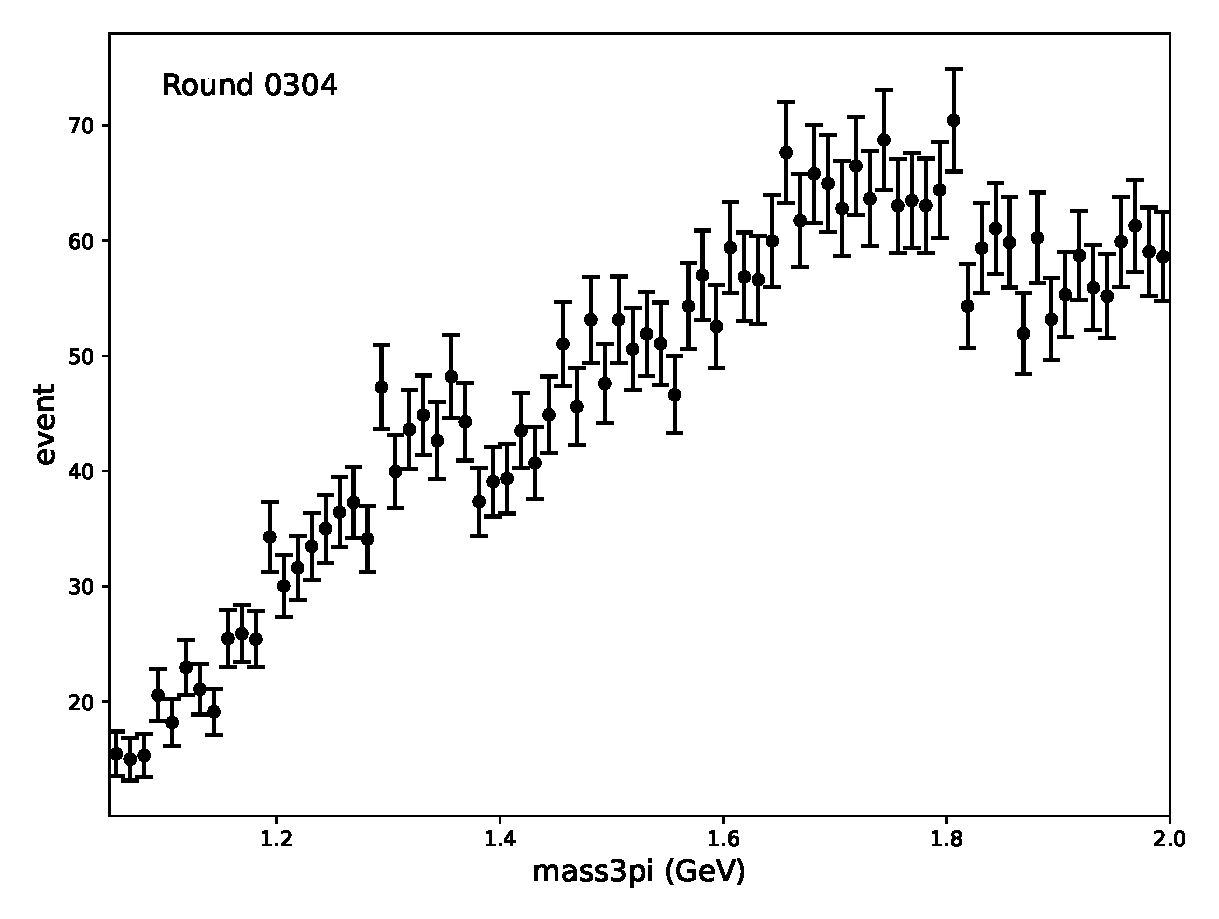
\includegraphics[width=0.32\textwidth]{fig/nonisr4pi_round0304_region3_plot.eps}
    \label{fig:nonisr4pi_r0304_region3}
}

\vspace{0.5\baselineskip}

% === Row 2: Round 15 ===
\subfloat[Round 15, $\omega(782)$ region]{
    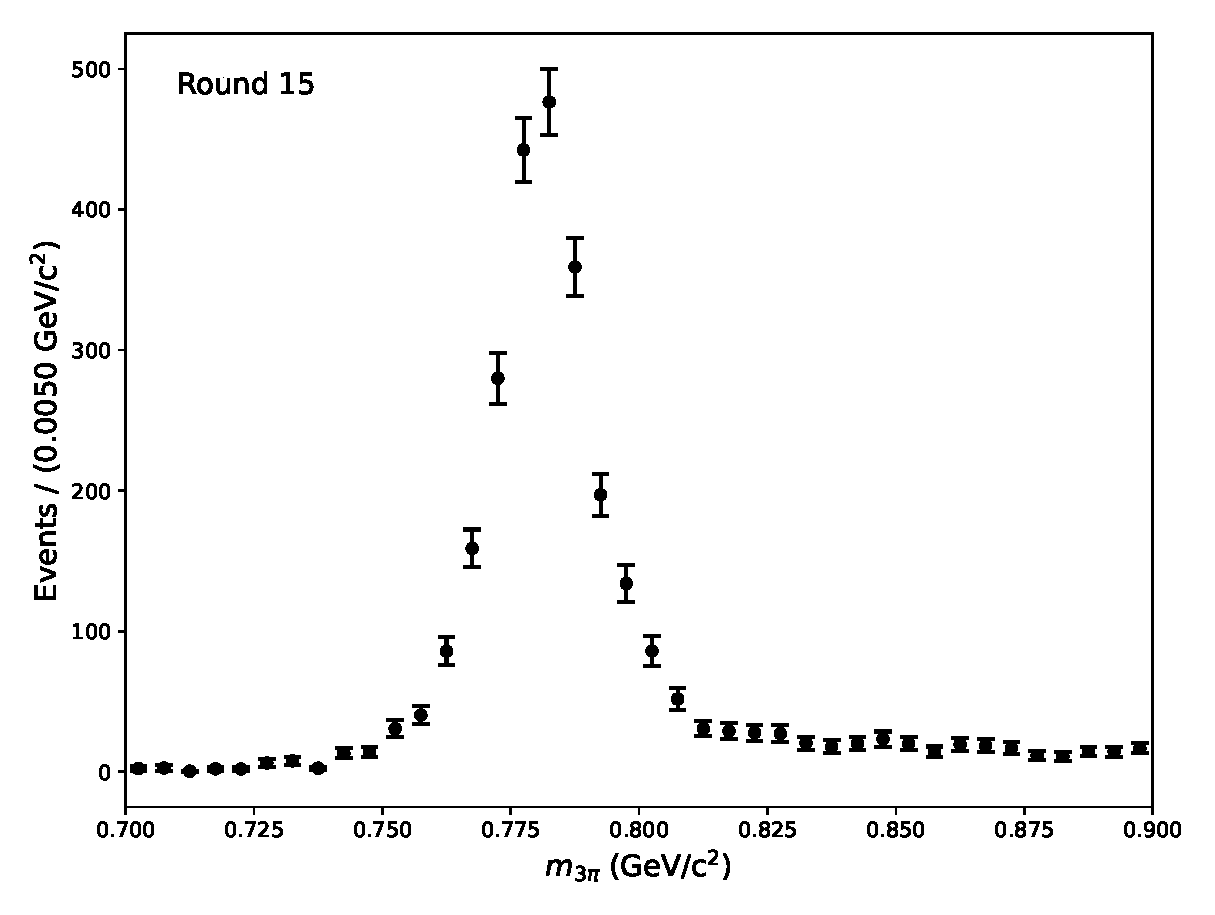
\includegraphics[width=0.32\textwidth]{fig/nonisr4pi_round15_region1_plot.eps}
    \label{fig:nonisr4pi_r15_region1}
}\hfill
\subfloat[Round 15, $\phi(1020)$ region]{
    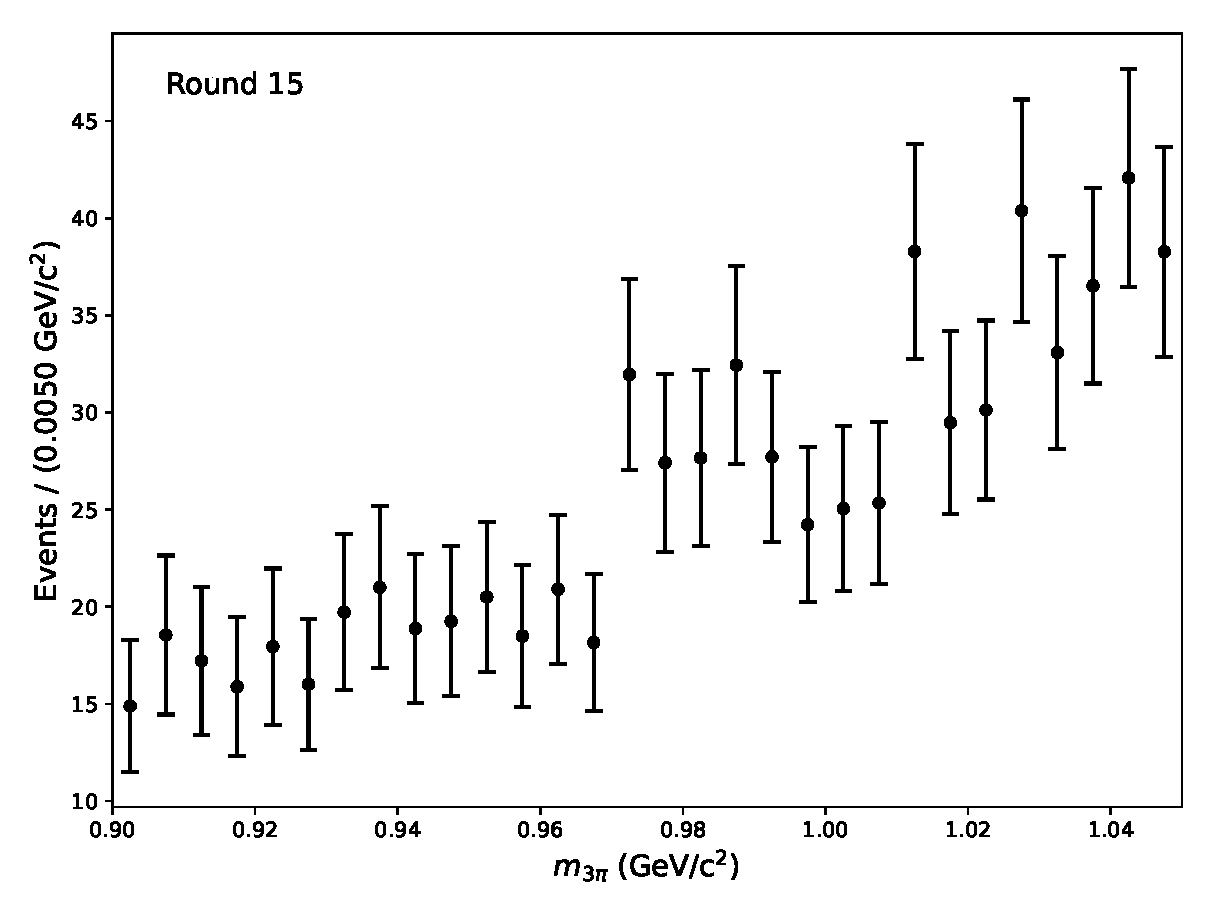
\includegraphics[width=0.32\textwidth]{fig/nonisr4pi_round15_region2_plot.eps}
    \label{fig:nonisr4pi_r15_region2}
}\hfill
\subfloat[Round 15, $\omega^{\prime}/\omega^{\prime\prime}$ region]{
    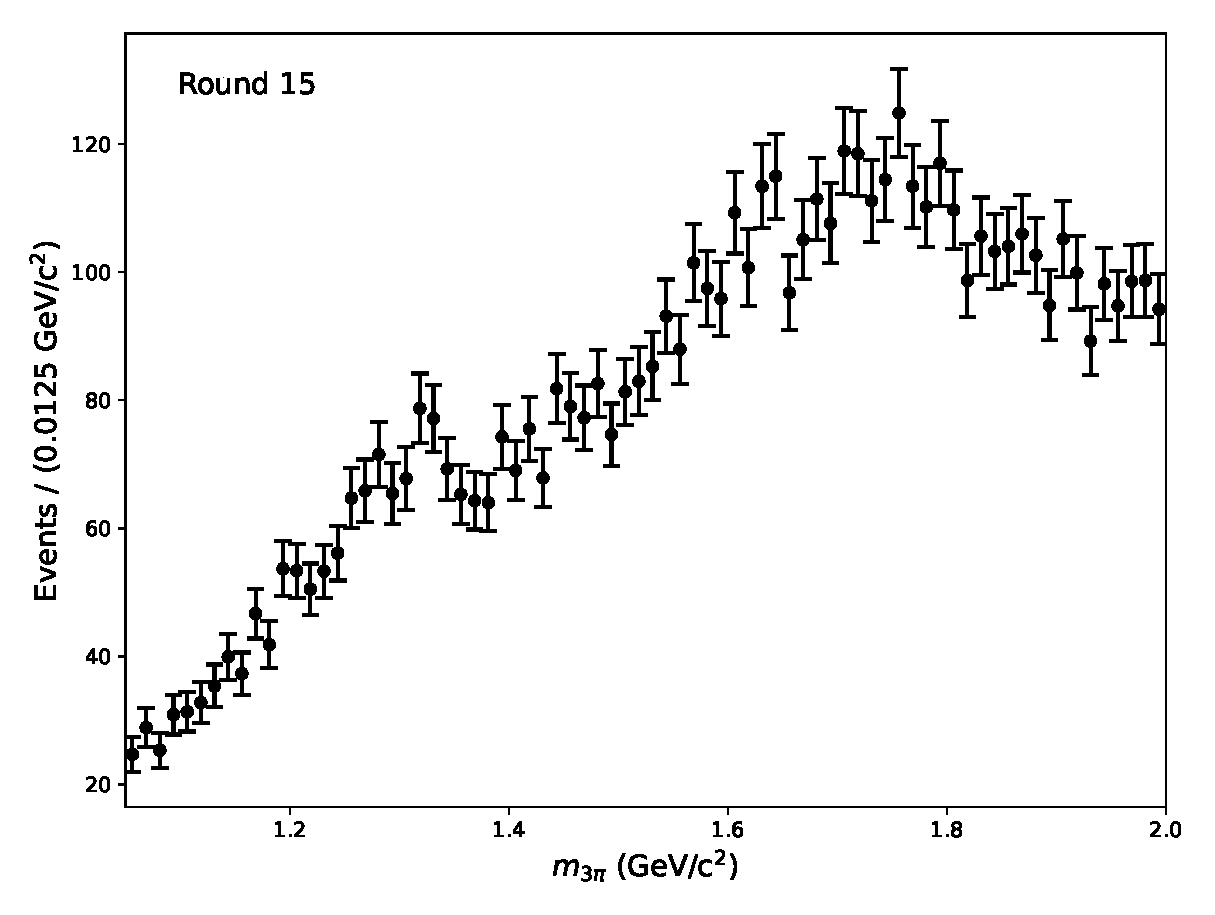
\includegraphics[width=0.32\textwidth]{fig/nonisr4pi_round15_region3_plot.eps}
    \label{fig:nonisr4pi_r15_region3}
}

\vspace{0.5\baselineskip}

% === Row 3: Round 16 ===
\subfloat[Round 16, $\omega(782)$ region]{
    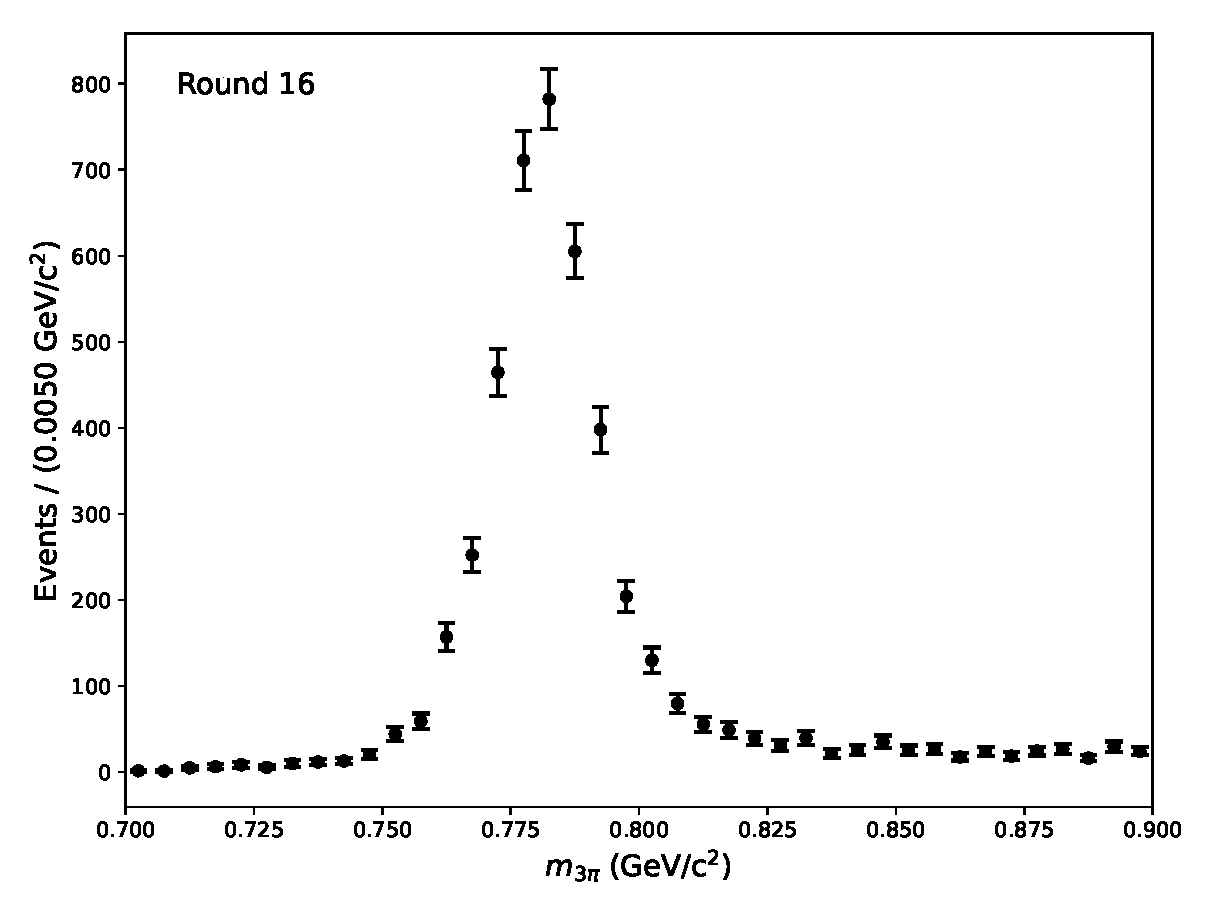
\includegraphics[width=0.32\textwidth]{fig/nonisr4pi_round16_region1_plot.eps}
    \label{fig:nonisr4pi_r16_region1}
}\hfill
\subfloat[Round 16, $\phi(1020)$ region]{
    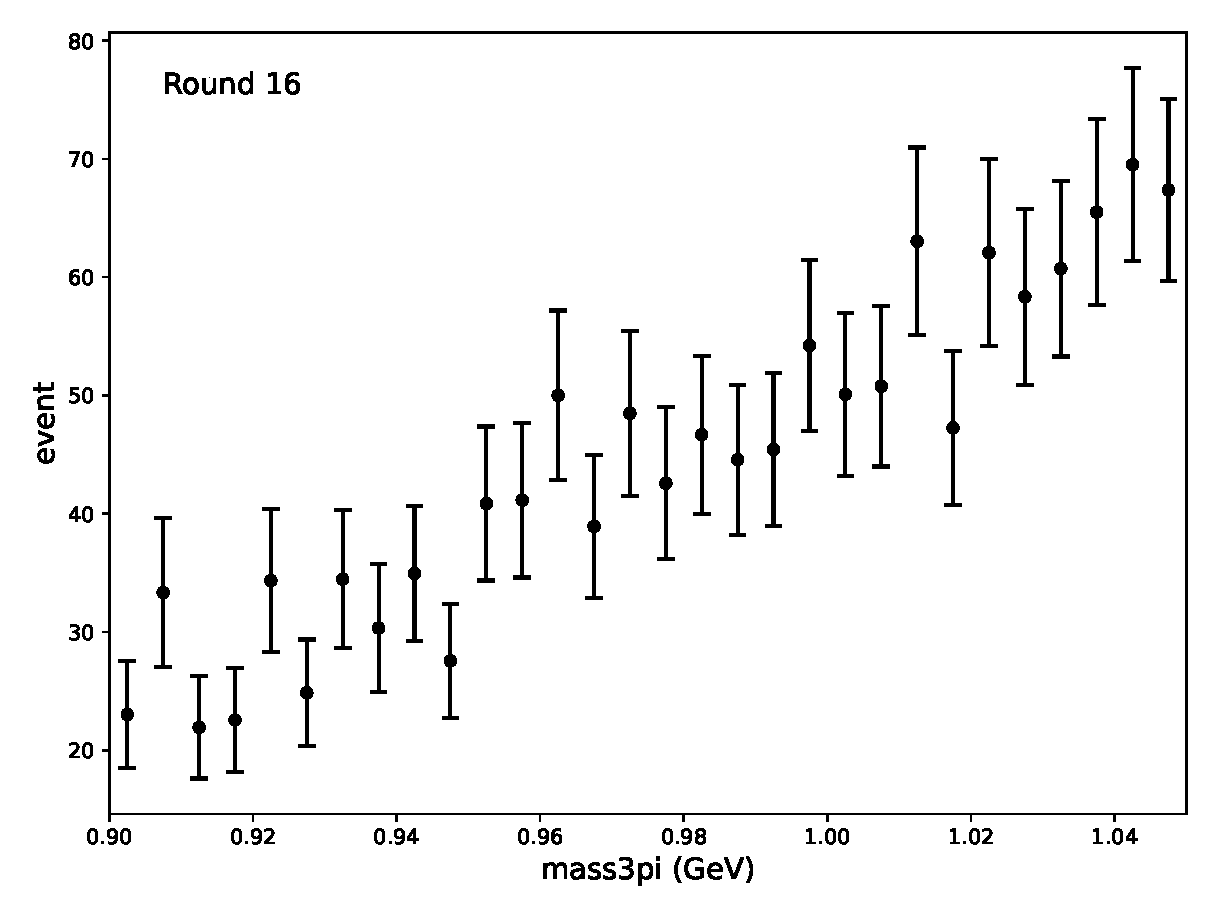
\includegraphics[width=0.32\textwidth]{fig/nonisr4pi_round16_region2_plot.eps}
    \label{fig:nonisr4pi_r16_region2}
}\hfill
\subfloat[Round 16, $\omega^{\prime}/\omega^{\prime\prime}$ region]{
    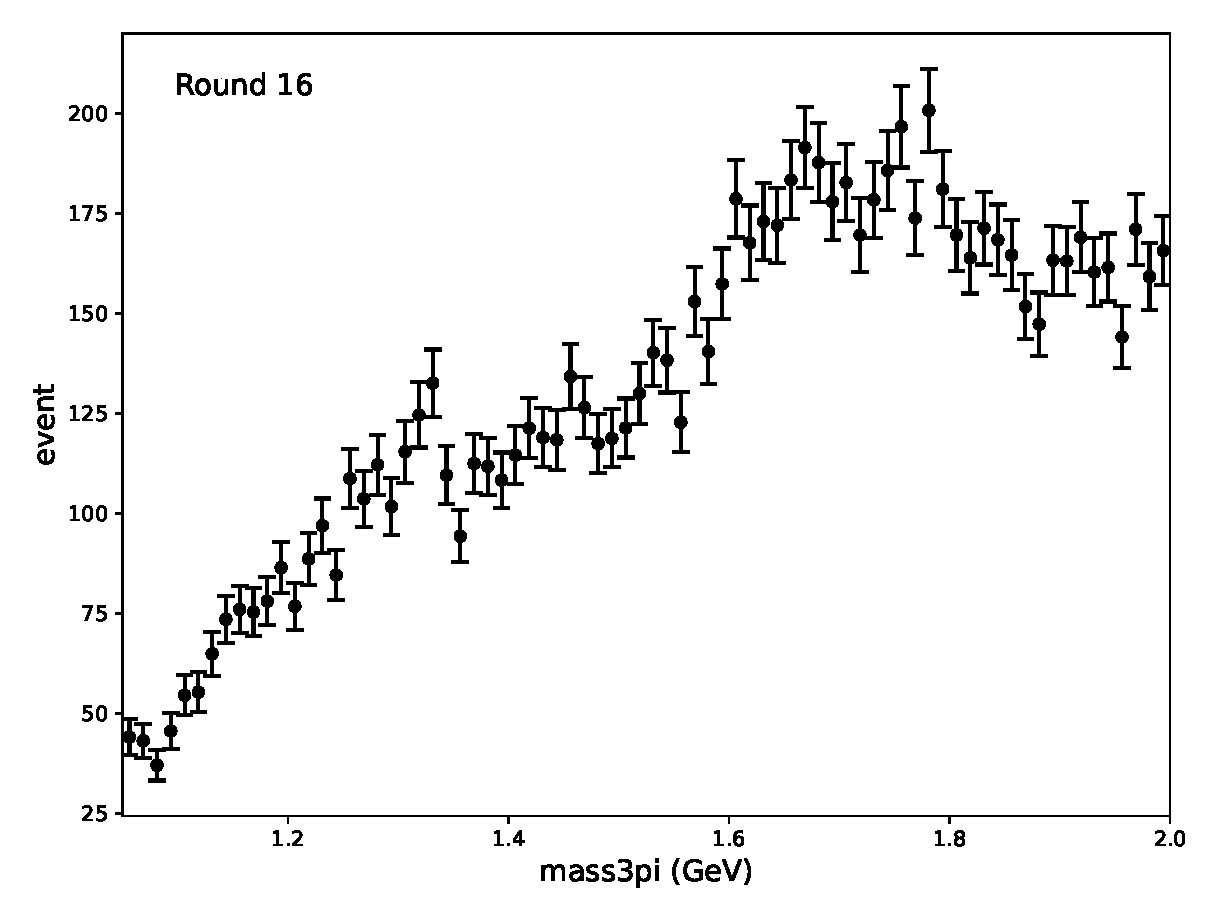
\includegraphics[width=0.32\textwidth]{fig/nonisr4pi_round16_region3_plot.eps}
    \label{fig:nonisr4pi_r16_region3}
}

\vspace{0.5\baselineskip}

% === Row 4: Round 17 ===
\subfloat[Round 17, $\omega(782)$ region]{
    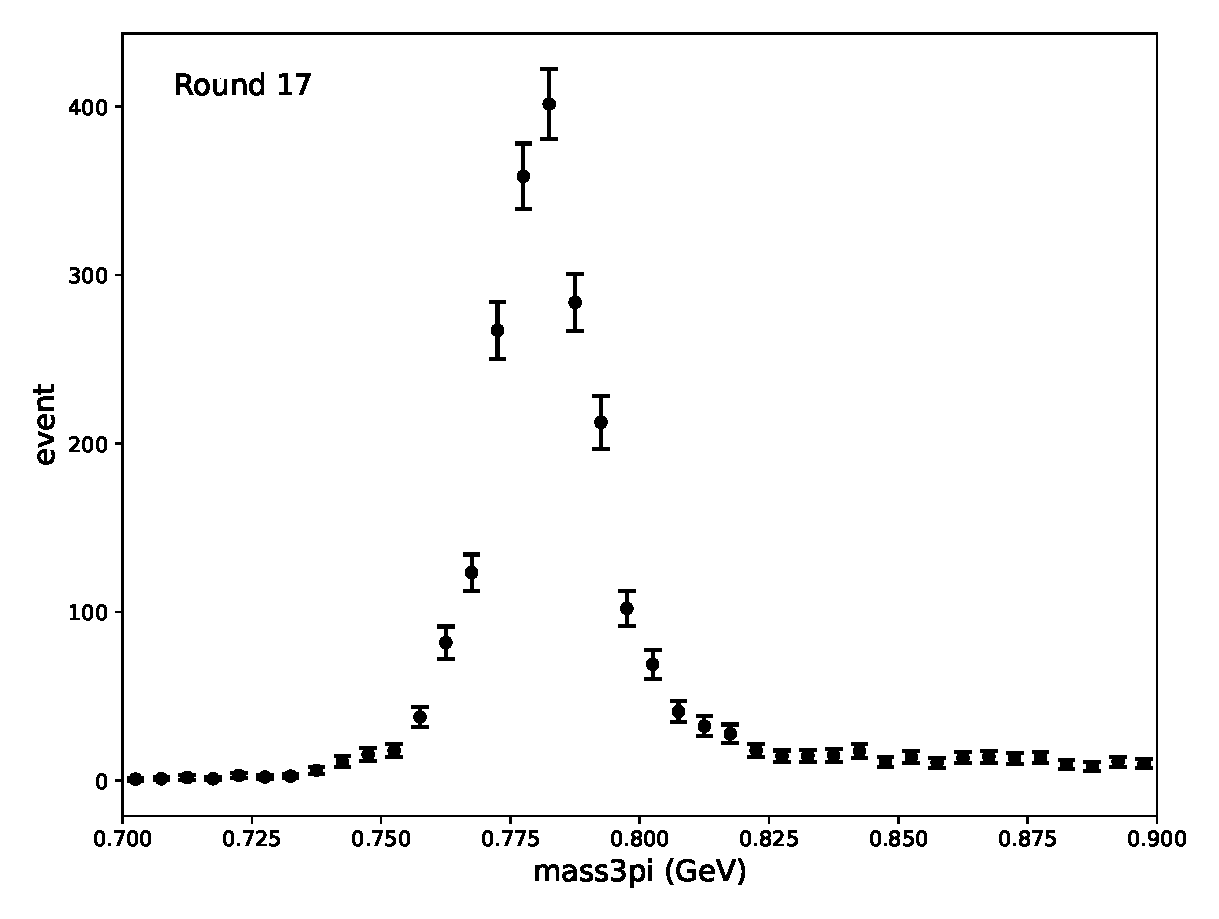
\includegraphics[width=0.32\textwidth]{fig/nonisr4pi_round17_region1_plot.eps}
    \label{fig:nonisr4pi_r17_region1}
}\hfill
\subfloat[Round 17, $\phi(1020)$ region]{
    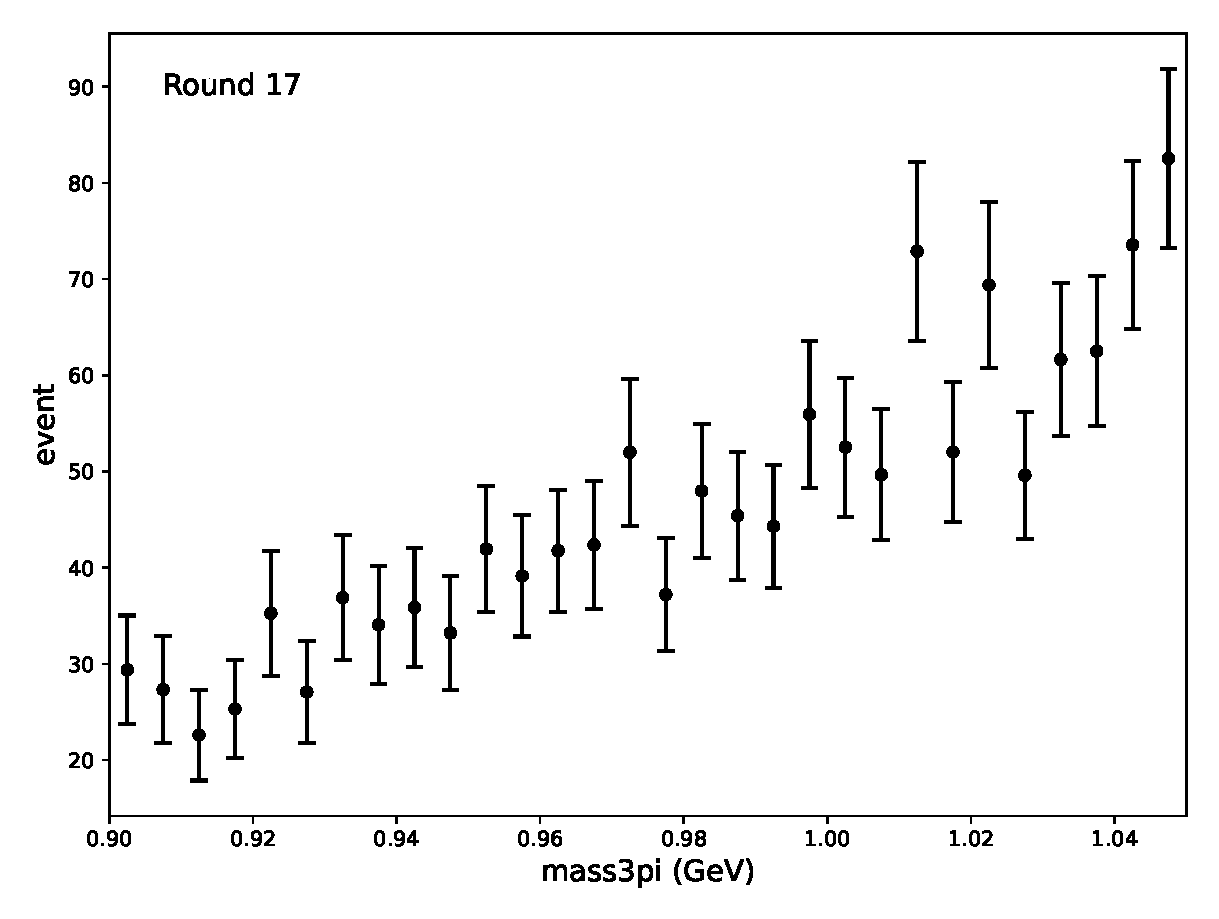
\includegraphics[width=0.32\textwidth]{fig/nonisr4pi_round17_region2_plot.eps}
    \label{fig:nonisr4pi_r17_region2}
}\hfill
\subfloat[Round 17, $\omega^{\prime}/\omega^{\prime\prime}$ region]{
    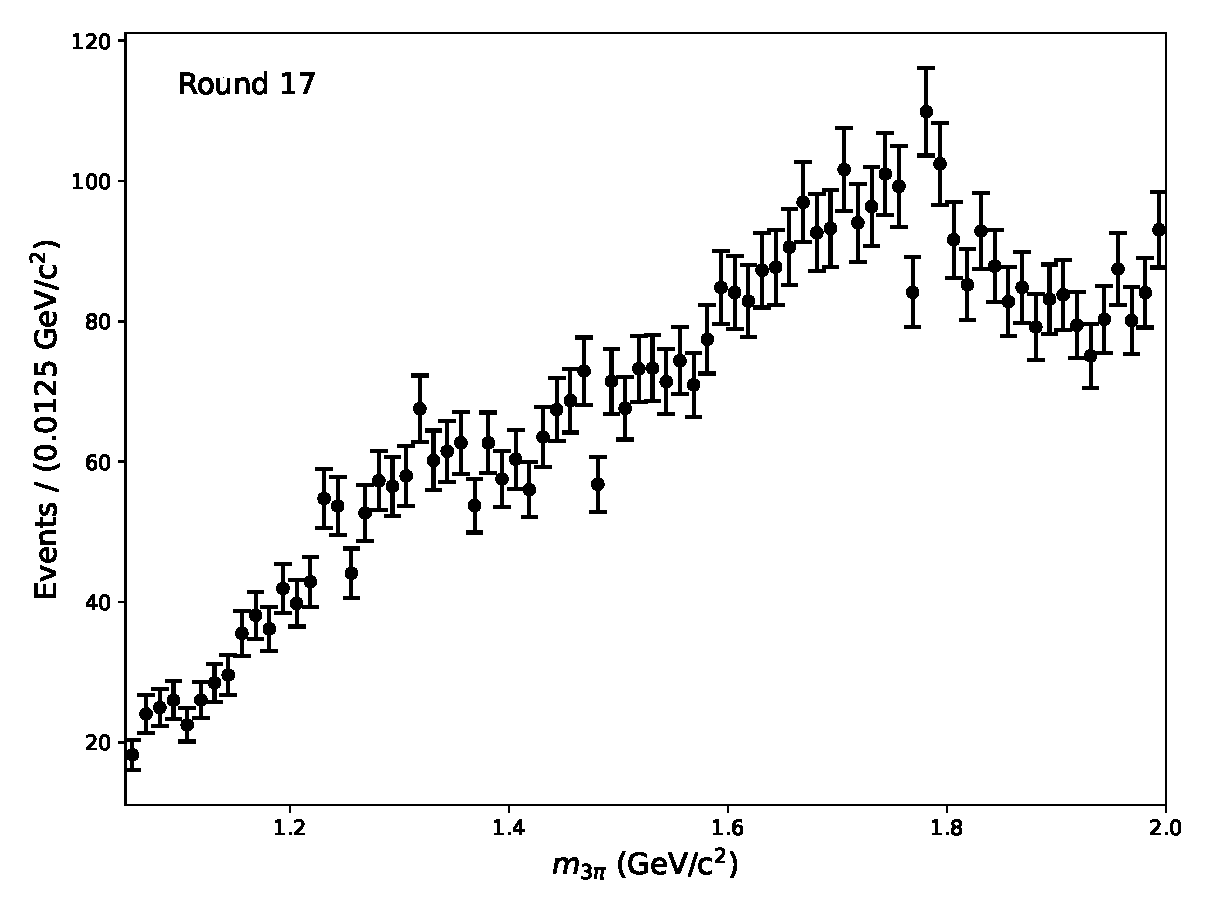
\includegraphics[width=0.32\textwidth]{fig/nonisr4pi_round17_region3_plot.eps}
    \label{fig:nonisr4pi_r17_region3}
}

\caption{Estimated background contributions from $e^{+}e^{-} \to \pi^{+}\pi^{-}\pi^{0}\pi^{0}$ in the signal region after scaling, shown for four data-taking periods. Each row corresponds to a different round: (a)--(c) Round~03/04, (d)--(f) Round~15, (g)--(i) Round~16, and (j)--(l) Round~17. The three columns represent different $3\pi$ invariant mass regions: $\omega(782)$ region (left), $\phi(1020)$ region (center), and higher-mass $\omega^{\prime}/\omega^{\prime\prime}$ region (right).}
\label{fig:nonisr4pi_all_rounds_regions}
\end{figure}

% \clearpage
% \subsection{Estimate of $\ee\to\pip\pim\piz\piz\gamma_{\text{ISR}}$}
% The second dominant background, $e^{+}e^{-} \to \gamma_{\mathrm{ISR}}\pi^{+}\pi^{-}\pi^{0}\pi^{0}$, is estimated using an analogous data-driven approach. The selection follows a similar dual-tag strategy to obtain a sample. The selection criteria are outlined below:

% Simultaneously, events must satisfy both the $e^{+}e^{-} \to \gamma_{\mathrm{ISR}}\pi^{+}\pi^{-}\pi^{0}\pi^{0}$ selection, where the $\gamma_{\mathrm{ISR}}$ is treated as an untagged missing momentum, and the tagged $e^{+}e^{-} \to \gamma_{\mathrm{ISR}}\pi^{+}\pi^{-}\pi^{0}$ loose selection criteria.

% \begin{itemize}
%     \item \textbf{$e^{+}e^{-} \to \gamma_{\mathrm{ISR}}\pi^{+}\pi^{-}\pi^{0}\pi^{0}$ Candidate Selection (Untagged $\gamma_{\mathrm{ISR}}$):}
%     \begin{itemize}
%         \item Exactly two good charged tracks.
%         \item $\text{nPi0} \geq 2$ \&\& $\text{nGoodShowers} \geq 4$ (requiring at least two $\pi^{0}$s).
%         \item The $\gamma_{\mathrm{ISR}}$ is not explicitly reconstructed from a shower. Instead, its 4-momentum is inferred as a \textit{missing} component within the kinematic fit.
%         \item A total 4-momentum constraint to the initial $e^{+}e^{-}$ collision is applied (4C fit).
%         \item The candidate with the minimum $\chi_{\mathrm{4C}}^2$ is chosen.
%         \item A requirement of $|\cos\theta_{\text{Miss}}| > 0.99$ is applied to the direction of the missing 4-momentum to ensure it is consistent with an ISR photon along the beam axis.
%         \item A kinematic fit quality cut of $\chi_{\mathrm{KF}}^2 < 10$ is applied.
%     \end{itemize}
%     \item \textbf{$\gamma_{\mathrm{ISR}}\pi^{+}\pi^{-}\pi^{0}$ Candidate Selection (within the same event):}
%     \begin{itemize}
%         \item The same two good charged tracks.
%         \item $\text{nPi0} \geq 1$ \& \& $\text{nGoodShowers} \geq 3$ (ensuring at least one $\pi^{0}$ and one photon tagged as $\gamma_{\mathrm{ISR}}$).
%         \item A total 4-momentum constraint to the initial $e^{+}e^{-}$ collision is applied (4C fit).
%         \item The candidate with the minimum $\chi_{\mathrm{4C}}^2$ is chosen.
%         \item No additional kinematic fit $\chi^2$ requirement is applied.
%     \end{itemize}
% \end{itemize}

% The application of this dual-tag selection strategy results in a highly pure sample of $e^{+}e^{-} \to \gamma_{\mathrm{ISR}}\pi^{+}\pi^{-}\pi^{0}\pi^{0}$ events. The high purity observed is a consequence of the stringent criteria. The corresponding $3\pi$ invariant mass distribution from this sample, which will be used as the input template for background estimation, is shown in Fig.~\ref{fig:isr4pi_background_spectrum}.

% \begin{figure}[htbp]
%     \centering
%     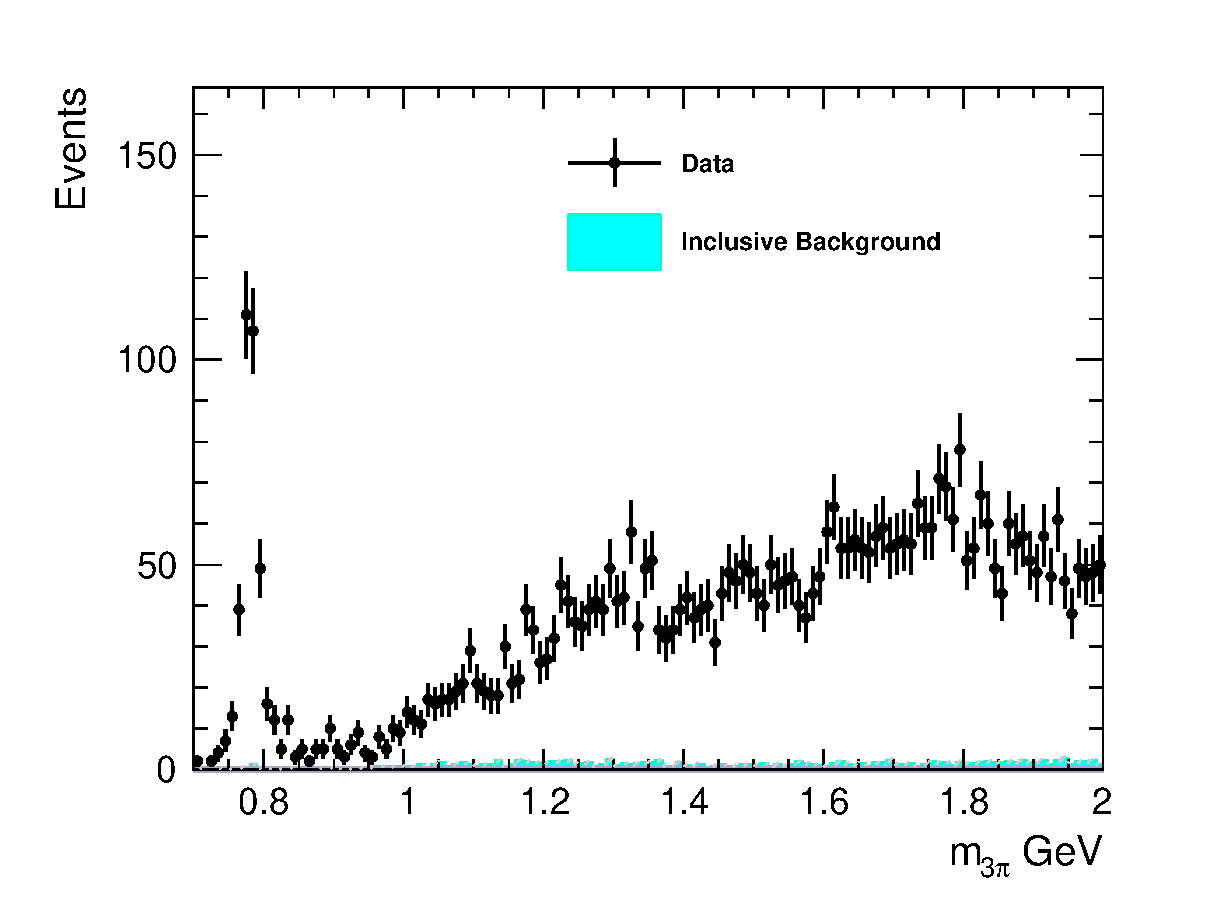
\includegraphics[width=0.45\textwidth]{fig/isr4pi_3pi_mass.eps}
%     \caption{The $3\pi$ invariant mass spectrum from selected $e^{+}e^{-} \to \gamma_{\mathrm{ISR}}\pi^{+}\pi^{-}\pi^{0}\pi^{0}$ events (green points) using data from round 16. The distribution is obtained after applying the dual-tag selection and serves as a clean template for background estimation.}
%     \label{fig:isr4pi_background_spectrum}
% \end{figure}

% As can be seen in Fig.~\ref{fig:isr4pi_background_spectrum}, the background contamination within this selected sample is negligible. Therefore, the inclusive background histogram is subtracted from the data histogram in a symbolic manner to obtain the pure $e^{+}e^{-} \to \gamma_{\mathrm{ISR}}\pi^{+}\pi^{-}\pi^{0}\pi^{0}$ event yield.

% The observed distribution will be similarly scaled by the appropriate efficiency ratio $R' = \epsilon_{\text{bkg}}' / \epsilon_{\text{sig}}'$ to estimate its contribution in the signal region. The resulting scaled background distributions in the three $3\pi$ invariant mass regions are presented in Fig.~\ref{fig:isr4pi_all_regions}.

% % 添加结果图（三个物理区域）
% \begin{figure}[htbp]
%     \centering
%     \subfloat[$\omega(782)$ region]{
%         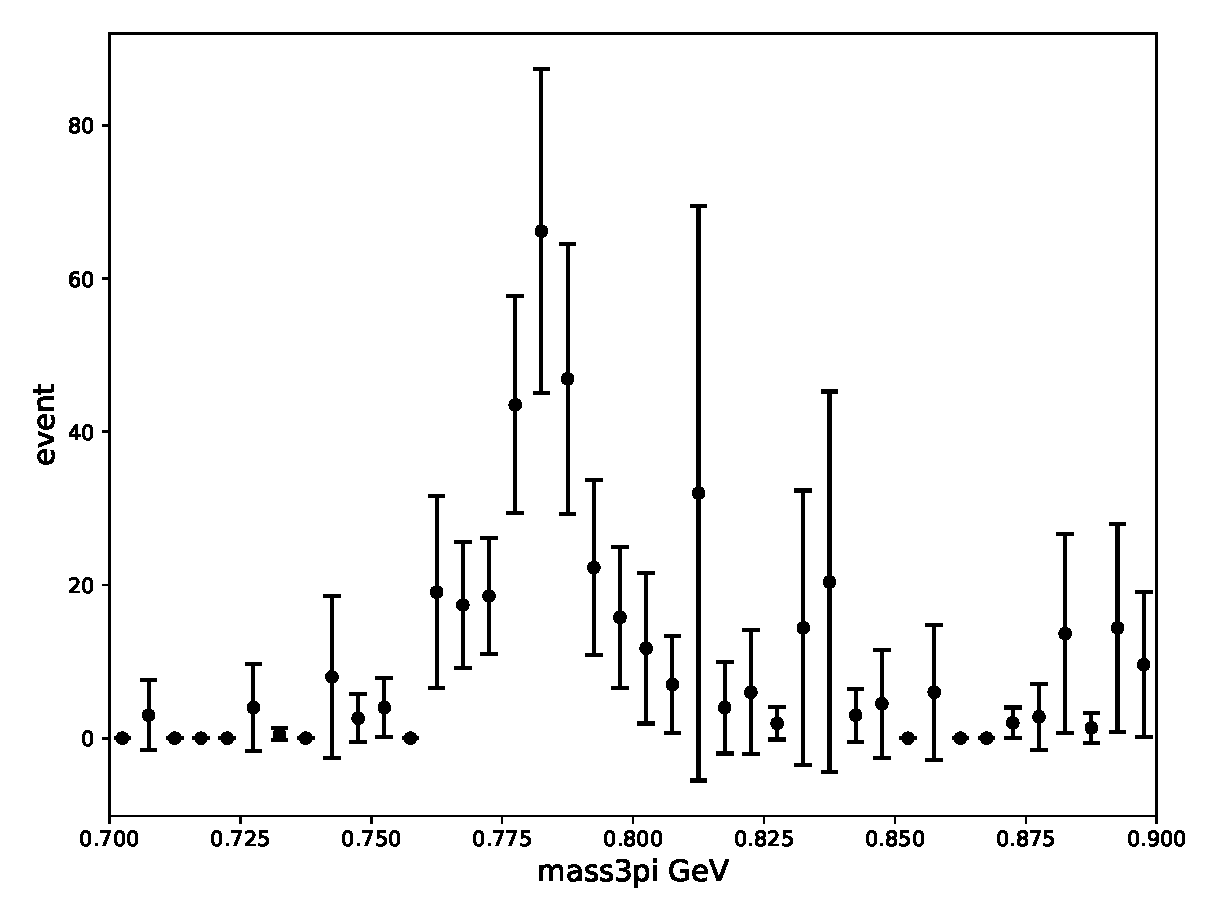
\includegraphics[width=0.32\textwidth]{fig/isr4pi_region1_plot.eps}
%         \label{fig:isr4pi_region1}
%     }
%     \hfill
%     \subfloat[$\phi(1020)$ region]{
%         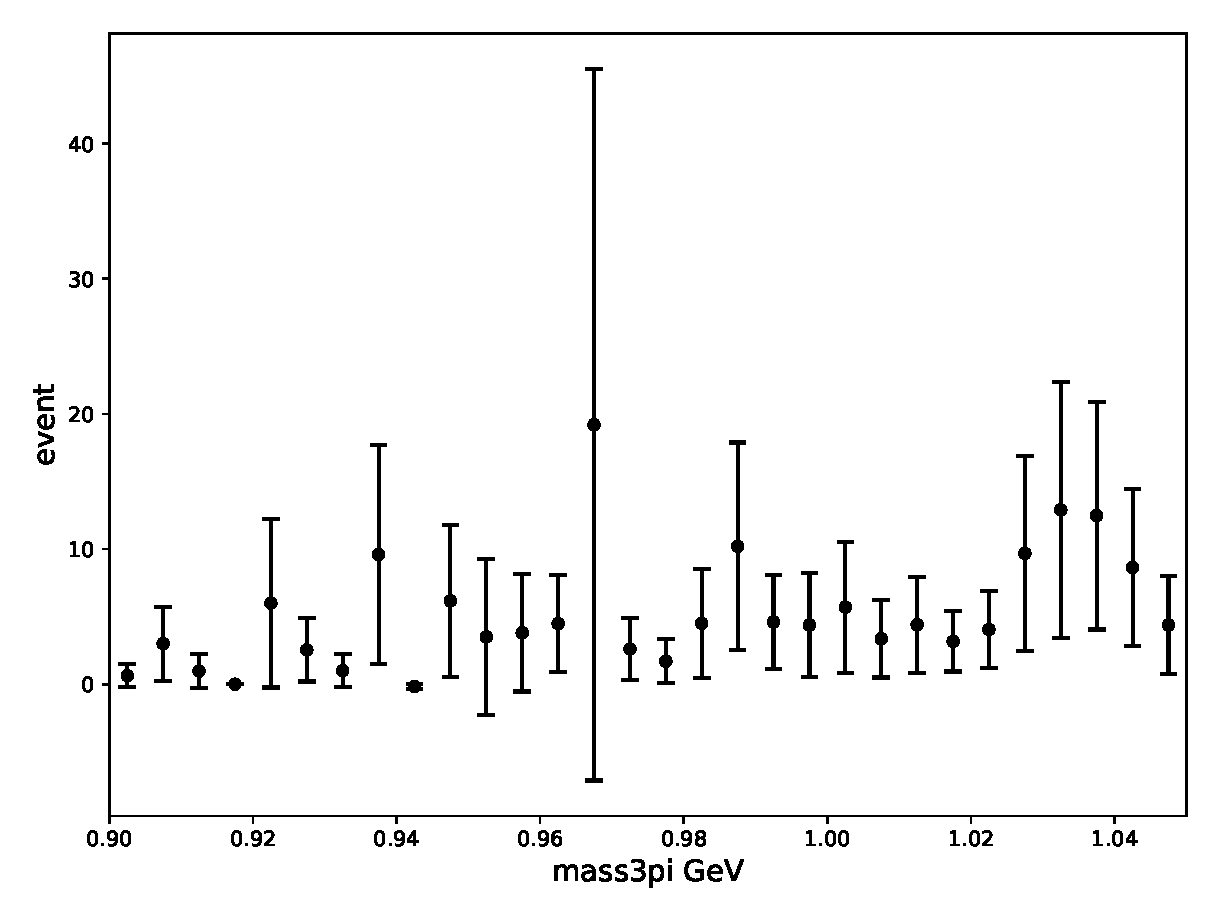
\includegraphics[width=0.32\textwidth]{fig/isr4pi_region2_plot.eps}
%         \label{fig:isr4pi_region2}
%     }
%     \hfill
%     \subfloat[$\omega^{\prime}$ and $\omega^{\prime\prime}$ region]{
%         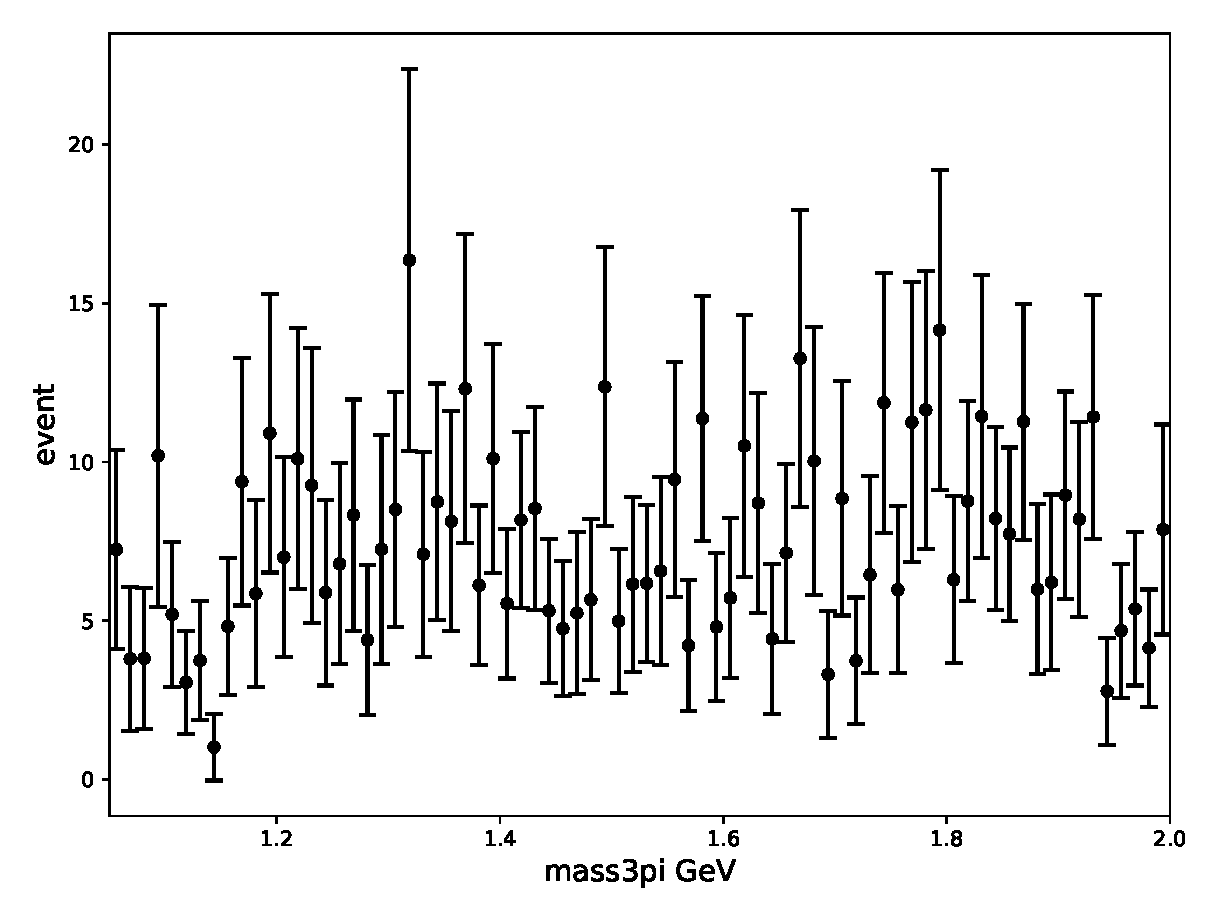
\includegraphics[width=0.32\textwidth]{fig/isr4pi_region3_plot.eps}
%         \label{fig:isr4pi_region3}
%     }
%     \caption{Estimated background contributions from $e^{+}e^{-} \to \gamma_{\mathrm{ISR}}\pi^{+}\pi^{-}\pi^{0}\pi^{0}$ in the signal region after scaling, using data from round 16. The three panels correspond to different $3\pi$ invariant mass regions: (a) the $\omega(782)$ region, (b) the $\phi(1020)$ region, and (c) the higher-mass $\omega^{\prime}/\omega^{\prime\prime}$ region.}
%     \label{fig:isr4pi_all_regions}
% \end{figure}

\clearpage
\subsection{Estimate of Other Backgrounds and Signal Yields}
\label{DataYields}
The estimation of the dominant peaking backgrounds from $e^{+}e^{-} \to
    \pi^{+}\pi^{-}\pi^{0}\pi^{0}$ has been completed in the previous subsection.
These backgrounds exhibit shapes similar to the signal resonance peaks and are
therefore categorized as peaking backgrounds.

In addition to the peaking component, a non-peaking continuum background
component must also be accounted for in the analysis. The primary objective of
this study is to measure the cross section for $e^{+}e^{-} \to
    \pi^{+}\pi^{-}\pi^{0}$ via ISR. The ISR photon reduces the effective c.m.
energy, allowing the measurement of the signal yield in narrow intervals of the
$3\pi$ invariant mass ($M_{3\pi}$).

The $M_{3\pi}$ spectrum is divided into three physically motivated regions,
each subdivided into multiple bins for detailed study:
\begin{itemize}
    \item The $\omega(782)$ region ($0.7$–$0.9~\text{GeV}/c^{2}$), divided into 40 bins.
    \item The $\phi(1020)$ region ($0.9$–$1.05~\text{GeV}/c^{2}$), divided into 30 bins.
    \item The $\omega^{\prime}/\omega^{\prime\prime}$ region
          ($1.05$–$2.0~\text{GeV}/c^{2}$), divided into 76 bins.
\end{itemize}

For each small $M_{3\pi}$ interval, the signal yield is extracted through an
extended unbinned maximum-likelihood fit to the $U_{\text{miss}}$ distribution,
where $U_{\text{miss}}$ is defined as the difference between the missing energy
and the magnitude of the missing momentum ($U_{\text{miss}} = E_{\text{miss}} -
    |\vec{p}_{\text{miss}}|$). The fit model incorporates probability density
functions (PDFs) representing the signal and all background components.

To illustrate the composition of $U_{\text{miss}}$ distributions across
different $M_{3\pi}$ regions, the inclusive MC simulation is examined.
Figure~\ref{fig:inclusiveMC_umiss_examples} shows the $U_{\text{miss}}$
distributions for the full $\omega(782)$ region, the full $\phi(1020)$ region,
and the full $\omega^{\prime}/\omega^{\prime\prime}$ region respectively, with
the peaking background contribution from $e^{+}e^{-} \to
    \pi^{+}\pi^{-}\pi^{0}\pi^{0}$ stacked according to its expected yield. These
distributions demonstrate the characteristic features of each mass region that
motivate our fitting strategy.

\begin{figure}[htbp]
    \centering
    \subfloat[$\omega(782)$ region]{
        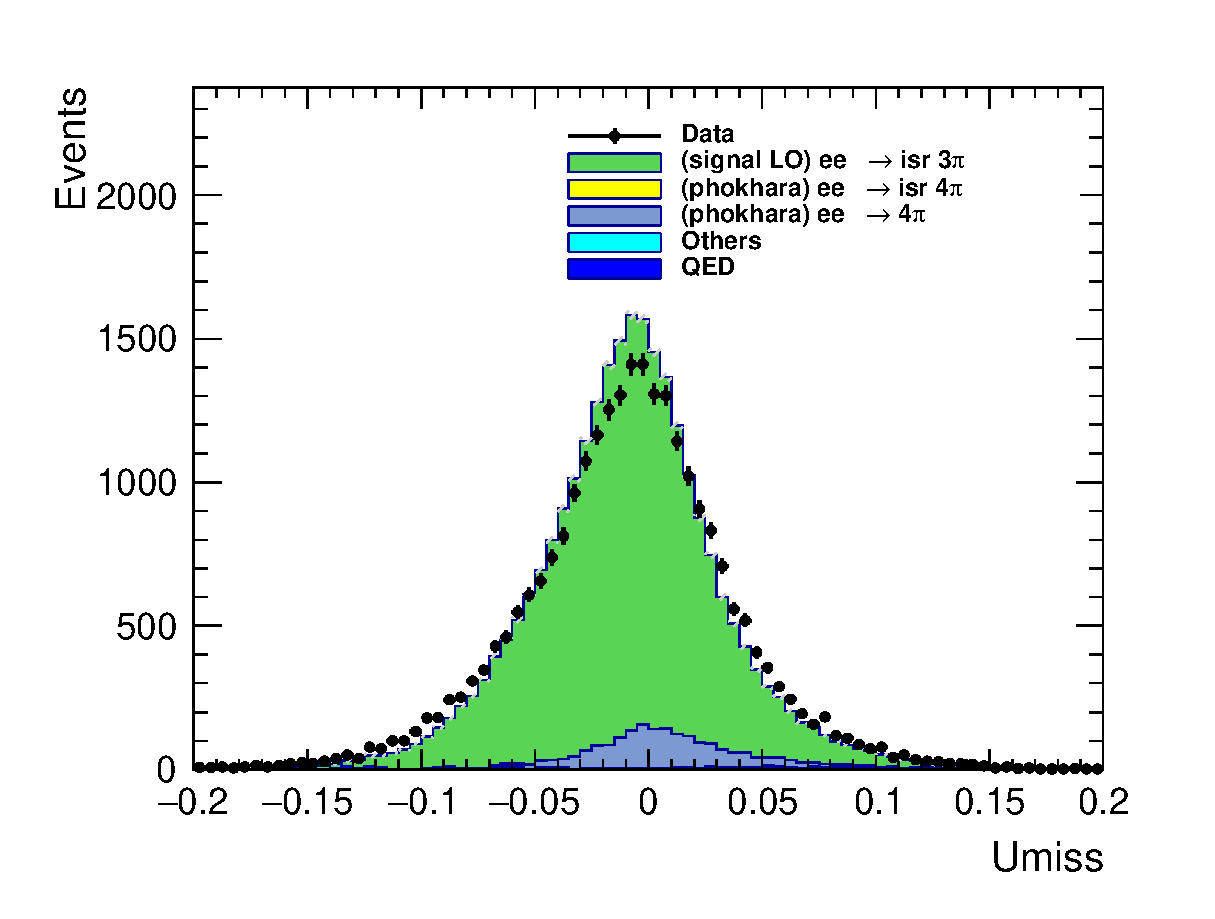
\includegraphics[width=0.32\textwidth]{fig/umiss_inclusiveMC_low.eps}
        \label{fig:umiss_inclusiveMC_low}
    }
    \hfill
    \subfloat[$\phi(1020)$ region]{
        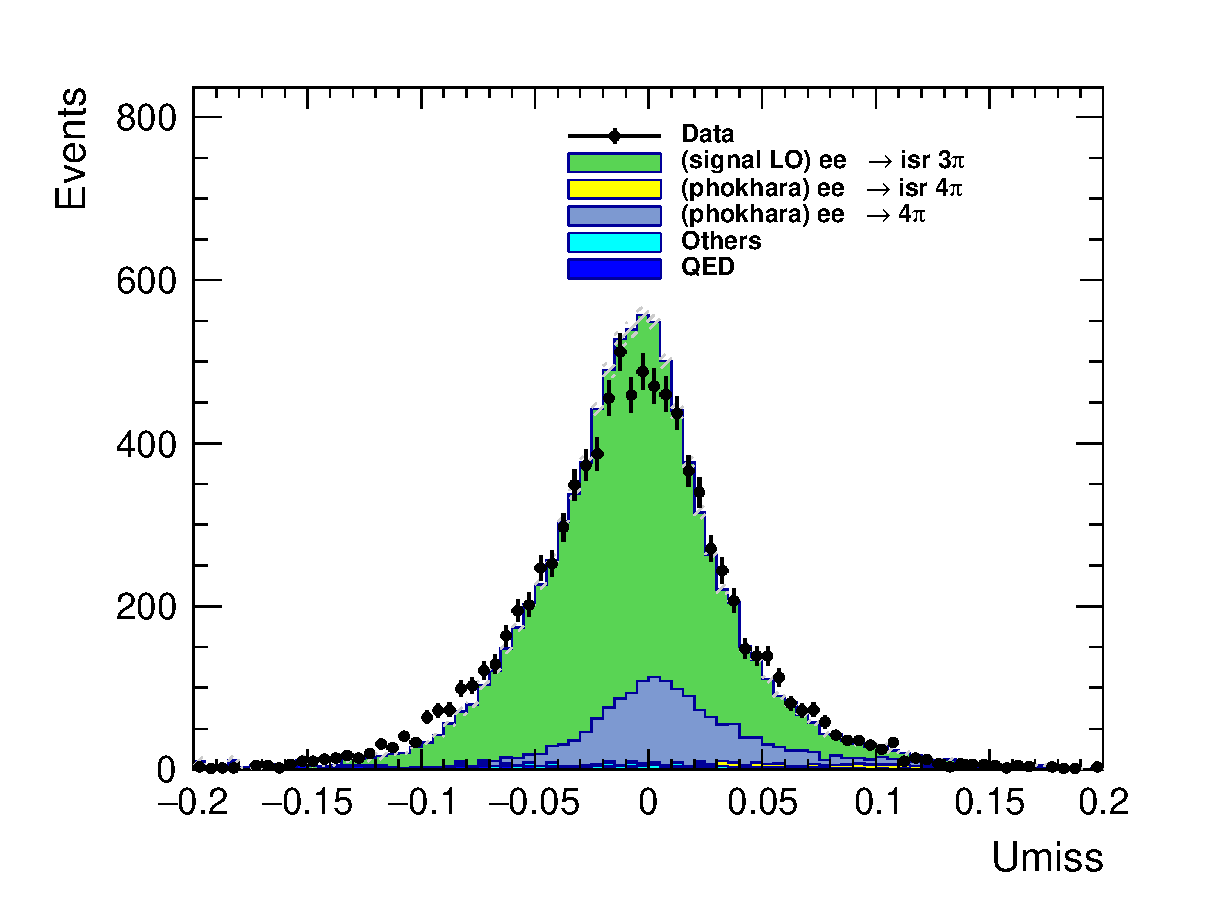
\includegraphics[width=0.32\textwidth]{fig/umiss_inclusiveMC_medium.eps}
        \label{fig:umiss_inclusiveMC_medium}
    }
    \hfill
    \subfloat[$\omega^{\prime}$ and $\omega^{\prime\prime}$ region]{
        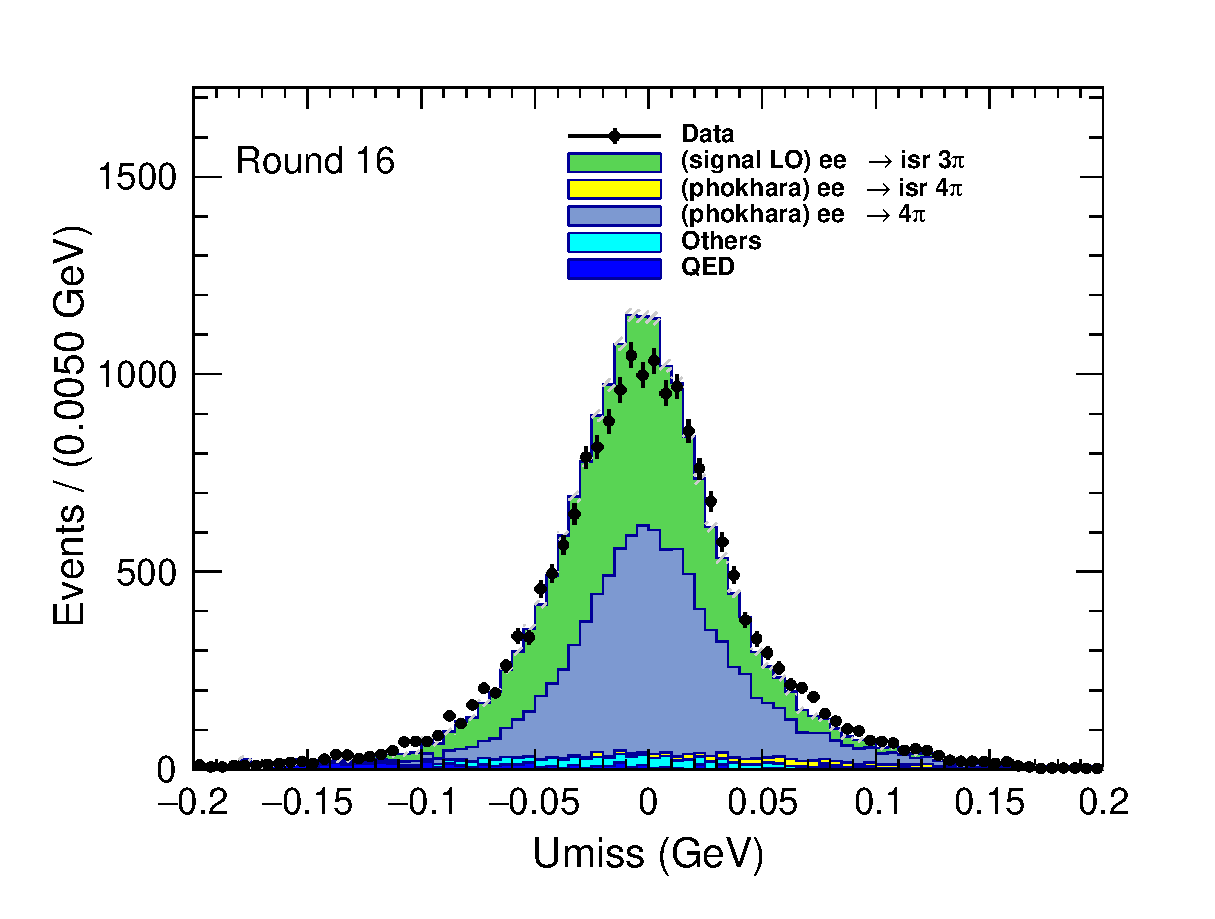
\includegraphics[width=0.32\textwidth]{fig/umiss_inclusiveMC_high.eps}
        \label{fig:umiss_inclusiveMC_high}
    }
    \caption{$U_{\text{miss}}$ distributions from inclusive MC simulation for three $M_{3\pi}$ regions: (a) the $\omega(782)$ region, (b) the $\phi(1020)$ region, and (c) the higher-mass $\omega^{\prime}/\omega^{\prime\prime}$ region.}
    \label{fig:inclusiveMC_umiss_examples}
\end{figure}

Based on the understanding from the inclusive MC, the PDFs for the fit are
constructed as follows:

\begin{itemize}
    \item \textbf{Signal PDF:} Histogram shape from signal MC, convolved with a Gaussian for resolution correction. The $\chi^{2}_{\mathrm{KF}}$ used in the $\chi^{2}_{\mathrm{KF}} < 50$ selection criterion has been corrected for data-MC differences in helix parameters as described in Section~\ref{sec:corr_signal_kmfit}.

    \item \textbf{Peaking background PDF:} Shape for $e^{+}e^{-} \to \pi^{+}\pi^{-}\pi^{0}\pi^{0}$ from dedicated MC, convolved with the same Gaussian as signal. Yield constrained by Gaussian term using data-driven estimate from Section~\ref{sec:bkg_stu}.

    \item \textbf{PDF shape sharing across bins:} Limited MC statistics preclude bin-by-bin shape extraction. Instead:
          \begin{itemize}
              \item For the $\omega(782)$ and $\phi(1020)$ regions, where the $M_{3\pi}$ bin width
                    is 5~MeV/$c^{2}$, the PDF shapes are extracted from MC simulation every five
                    consecutive bins, corresponding to 25~MeV/$c^{2}$ intervals. All five bins
                    within each such interval share the same PDF shape, under the assumption that
                    the $U_{\text{miss}}$ distribution varies slowly over this mass range.

              \item For the $\omega^{\prime}/\omega^{\prime\prime}$ region, where the $M_{3\pi}$
                    bin width is 12.5~MeV/$c^{2}$, the PDF shapes are also extracted every
                    25~MeV/$c^{2}$. Each extracted shape is therefore shared by two adjacent bins,
                    balancing the need for shape precision against the limited MC statistics in
                    this higher-mass region.
          \end{itemize}

    \item \textbf{Continuum background PDF:} All remaining minor background processes are collectively described by a polynomial function. A first-order polynomial (linear function) is used for the $\omega(782)$ and $\phi(1020)$ regions, while a second-order Chebyshev polynomial is employed for the $\omega^{\prime}/\omega^{\prime\prime}$ region, as suggested by the shape of the inclusive MC distribution in Fig.~\ref{fig:umiss_inclusiveMC_high}.
\end{itemize}

The fit procedure is validated by examining the quality of the fits to data in representative $M_{3\pi}$ bins across the three mass regions, using Round 16 as an illustrative example. Figure~\ref{fig:fit_examples} presents typical fit results for three selected bins, one from each region, demonstrating the ability of the fit model to accurately describe the data. The signal component, peaking background from $\pi^{+}\pi^{-}\pi^{0}\pi^{0}$, and polynomial continuum background are clearly distinguished, and the total PDF provides an excellent description of the data distribution in each case.

\begin{figure}[htbp]
    \centering
    \subfloat[Example bin in the $\omega(782)$ region]{
        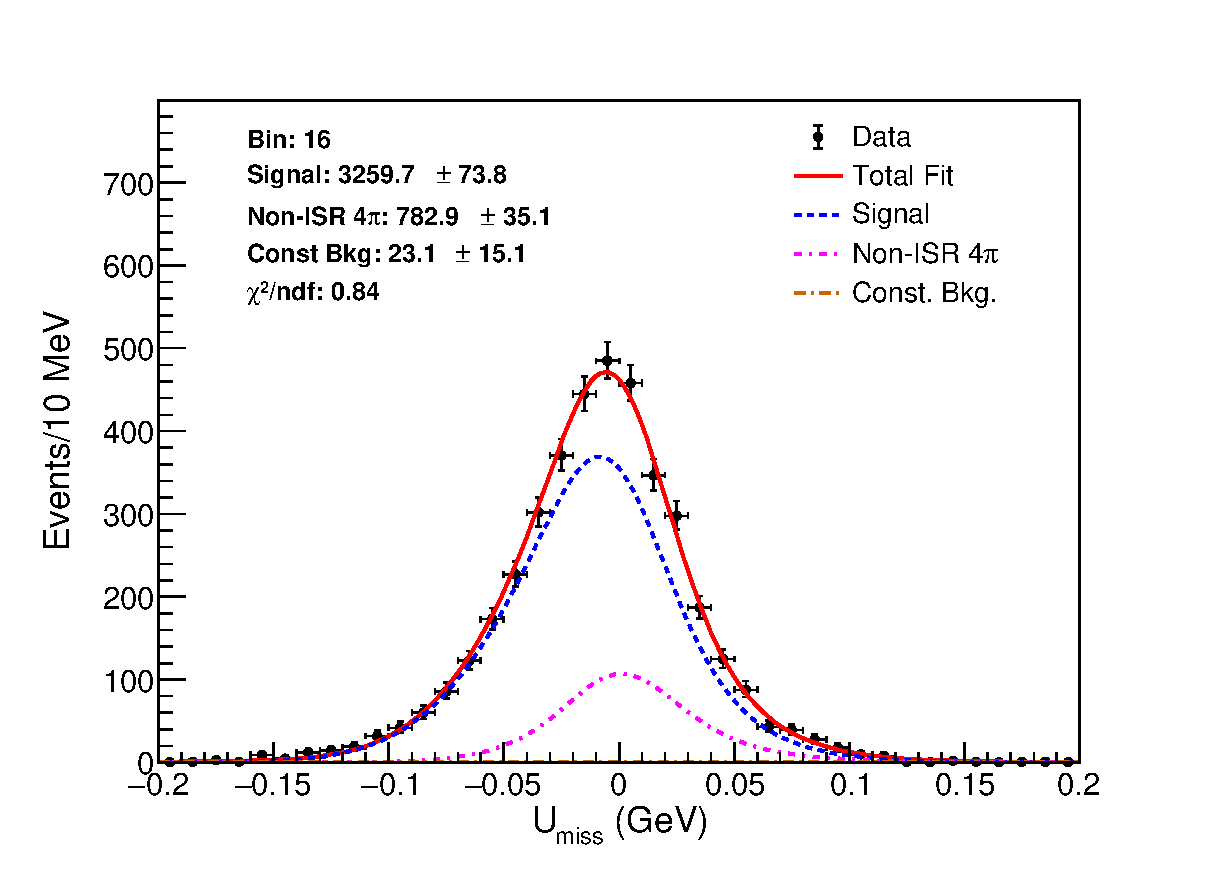
\includegraphics[width=0.32\textwidth]{fig/fit_example_omega.eps}
        \label{fig:fit_example_omega}
    }
    \hfill
    \subfloat[Example bin in the $\phi(1020)$ region]{
        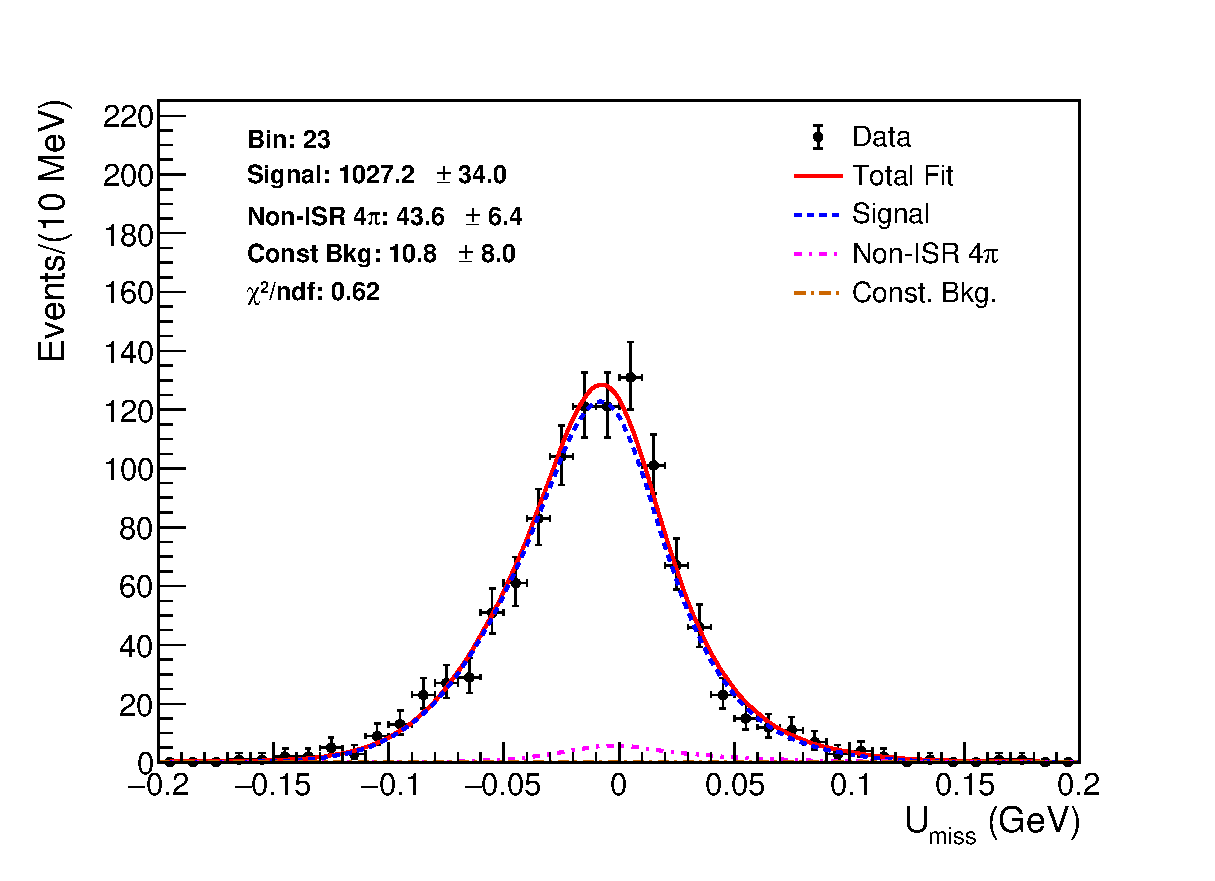
\includegraphics[width=0.32\textwidth]{fig/fit_example_phi.eps}
        \label{fig:fit_example_phi}
    }
    \hfill
    \subfloat[Example bin in the $\omega^{\prime}/\omega^{\prime\prime}$ region]{
        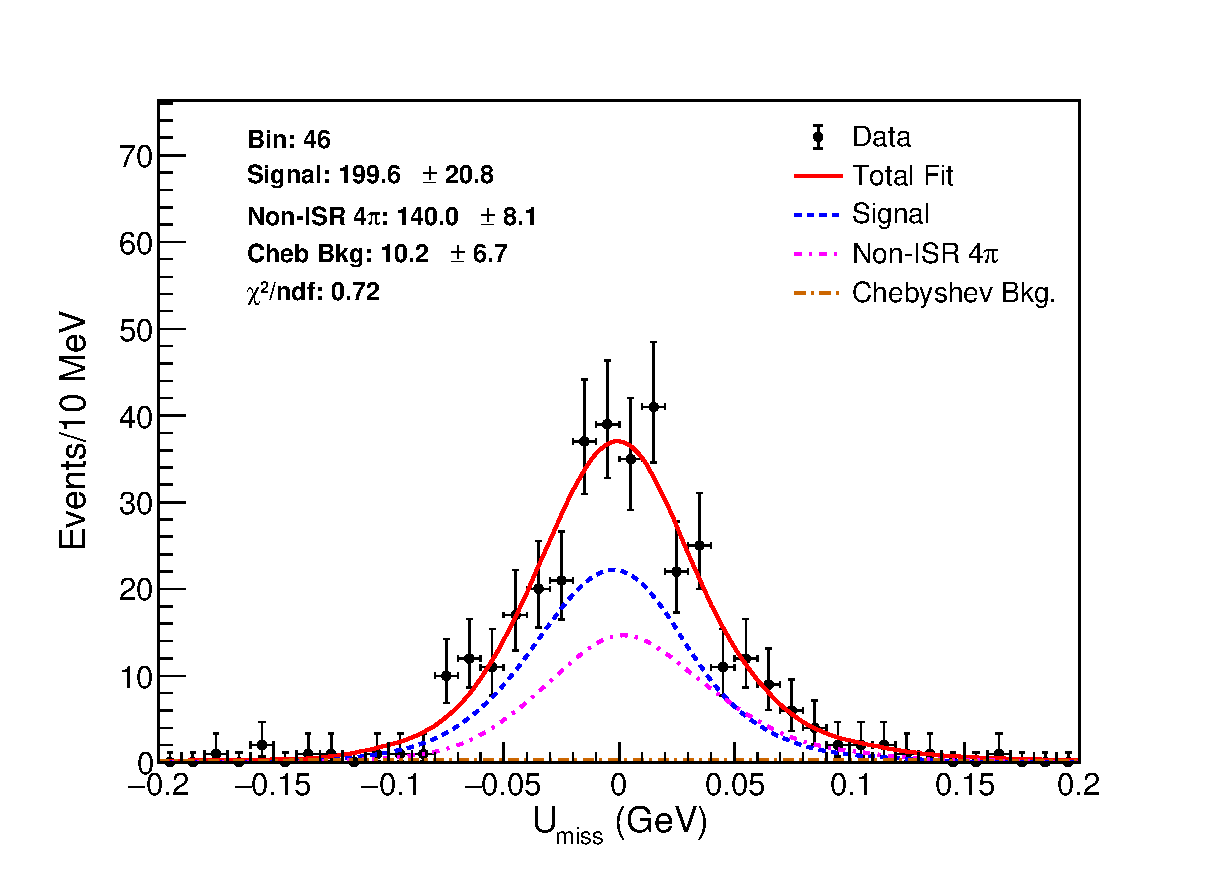
\includegraphics[width=0.32\textwidth]{fig/fit_example_high.eps}
        \label{fig:fit_example_high}
    }
    \caption{Typical $U_{\text{miss}}$ fit results for representative $M_{3\pi}$ bins from each of the three mass regions, shown for Round 16 data.}
    \label{fig:fit_examples}
\end{figure}

Applying this fitting procedure to all $M_{3\pi}$ bins yields the extracted signal yields across the entire mass spectrum. The same fit is performed independently for four data-taking periods: Round~03/04, Round~15, Round~16, and Round~17. Figure~\ref{fig:signal_yields} presents the measured signal yields as a function of $M_{3\pi}$ for all four periods, organized by the three mass regions. In each panel, the $\omega(782)$ resonance is clearly visible as a prominent peak around $0.78~\text{GeV}/c^{2}$, while the $\phi(1020)$ resonance appears as a distinct but smaller peak near $1.02~\text{GeV}/c^{2}$. In the higher mass regions, broad structures corresponding to the $\omega^{\prime}$ and $\omega^{\prime\prime}$ excitations are observed, with significantly reduced yields due to the decreasing cross section and lower ISR photon probability at larger momentum transfers. The results show good consistency across the four data-taking periods, with statistical uncertainties represented by the error bars.

\begin{figure}[htbp]
\centering

% === Row 1: Round 03/04 ===
\subfloat[Round 03/04, $\omega(782)$ region]{
    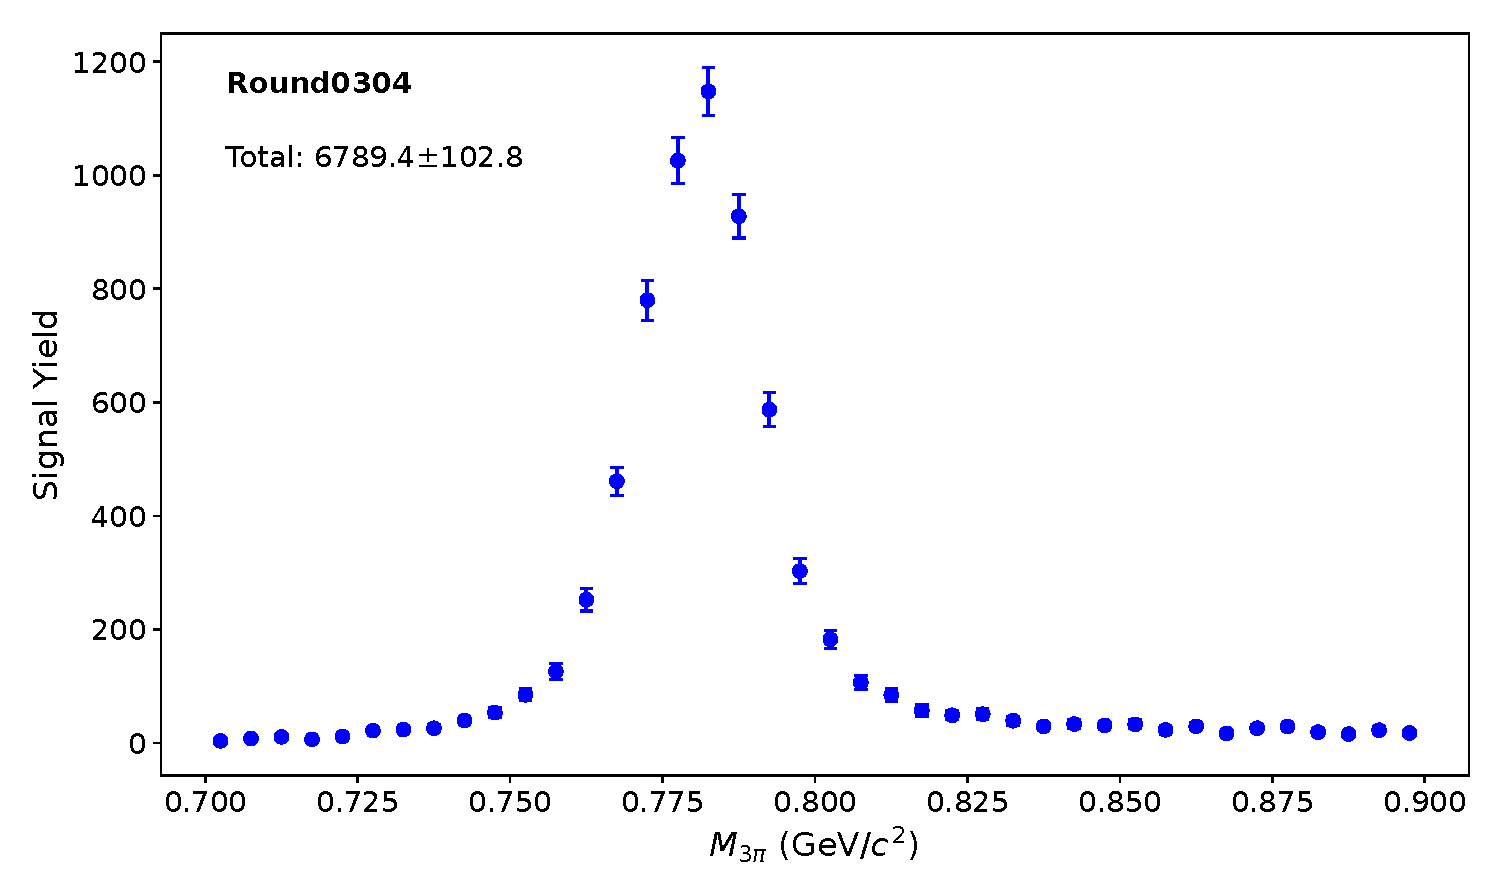
\includegraphics[width=0.32\textwidth]{fig/yields_round0304_region1.eps}
    \label{fig:yields_r0304_region1}
}\hfill
\subfloat[Round 03/04, $\phi(1020)$ region]{
    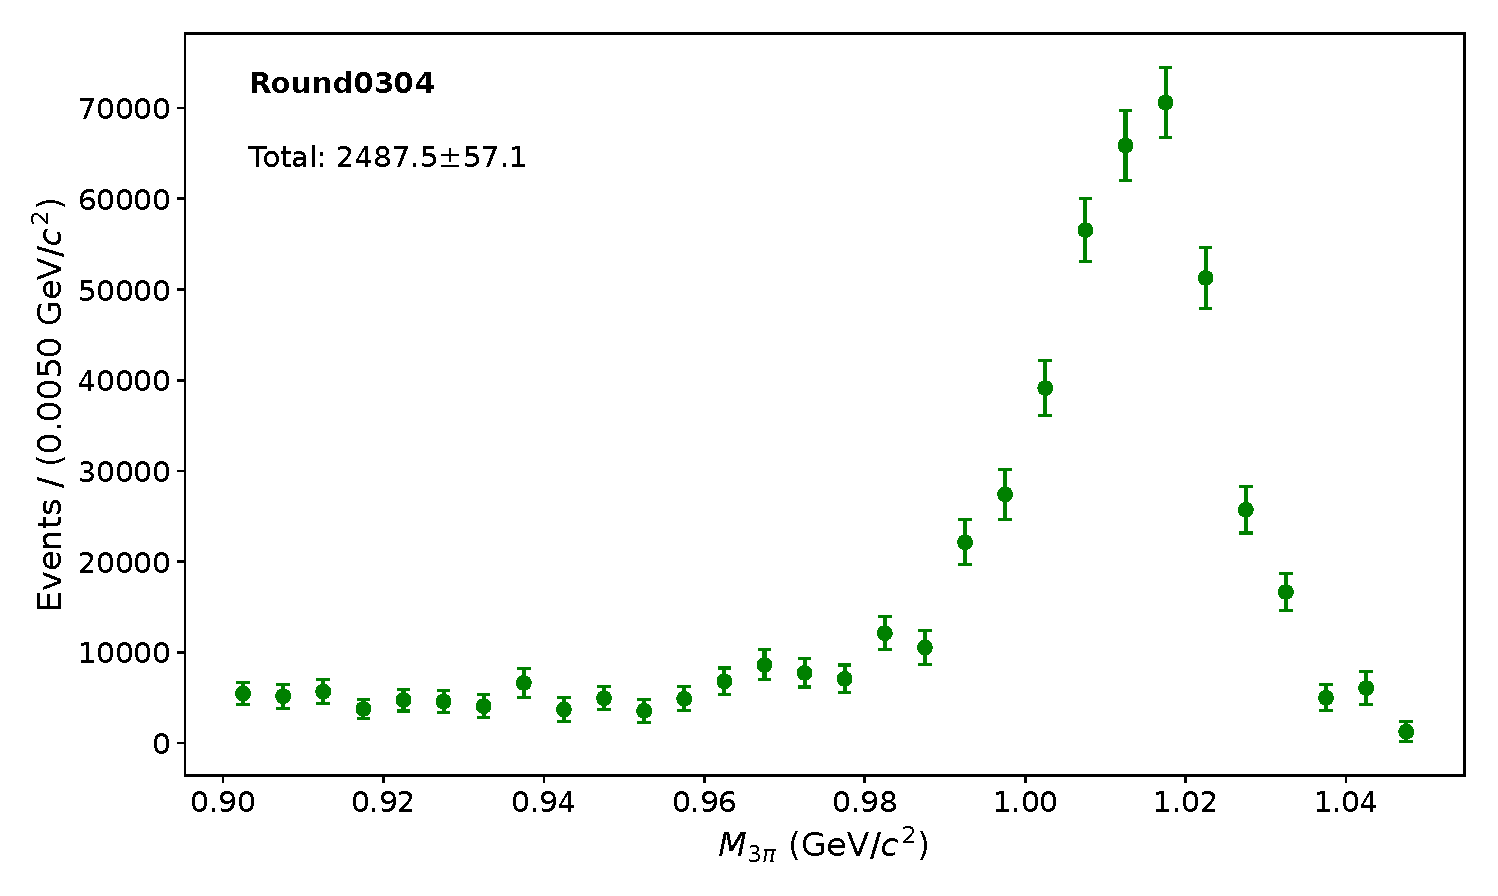
\includegraphics[width=0.32\textwidth]{fig/yields_round0304_region2.eps}
    \label{fig:yields_r0304_region2}
}\hfill
\subfloat[Round 03/04, $\omega^{\prime}/\omega^{\prime\prime}$ region]{
    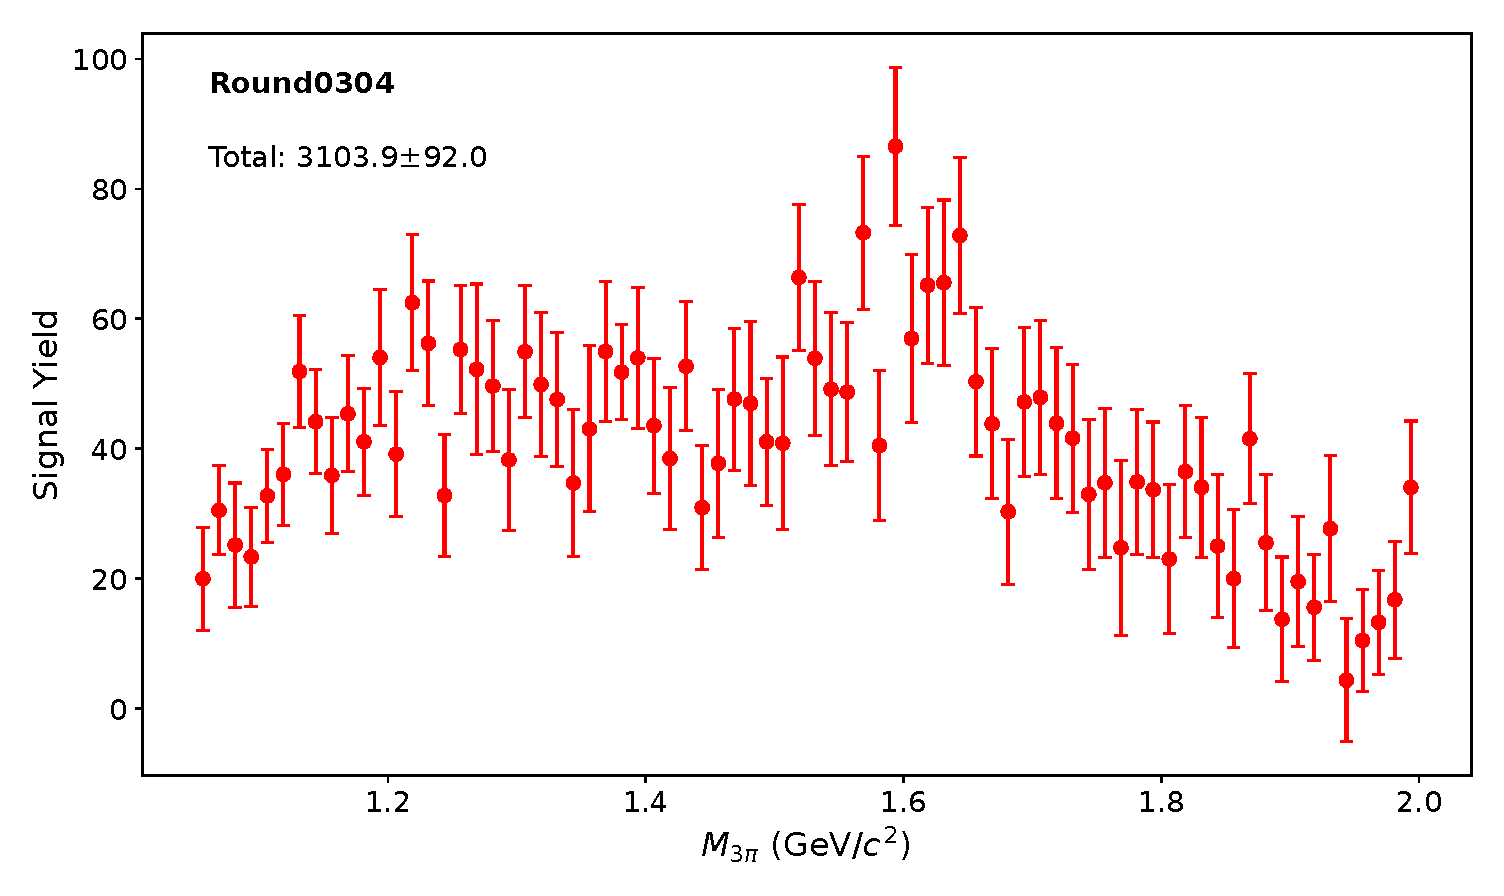
\includegraphics[width=0.32\textwidth]{fig/yields_round0304_region3.eps}
    \label{fig:yields_r0304_region3}
}

\vspace{0.5\baselineskip}

% === Row 2: Round 15 ===
\subfloat[Round 15, $\omega(782)$ region]{
    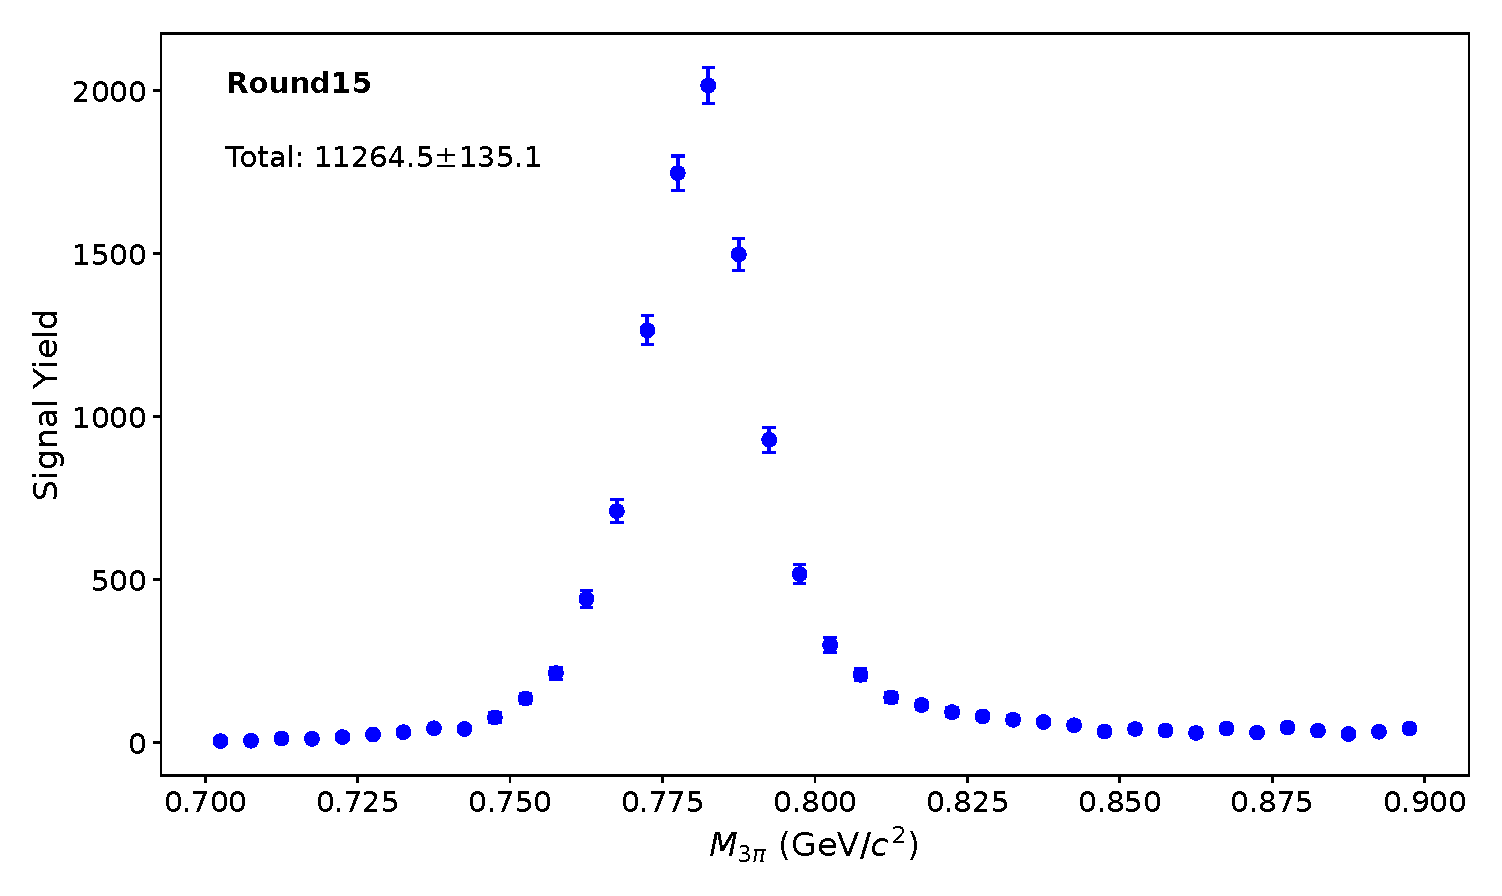
\includegraphics[width=0.32\textwidth]{fig/yields_round15_region1.eps}
    \label{fig:yields_r15_region1}
}\hfill
\subfloat[Round 15, $\phi(1020)$ region]{
    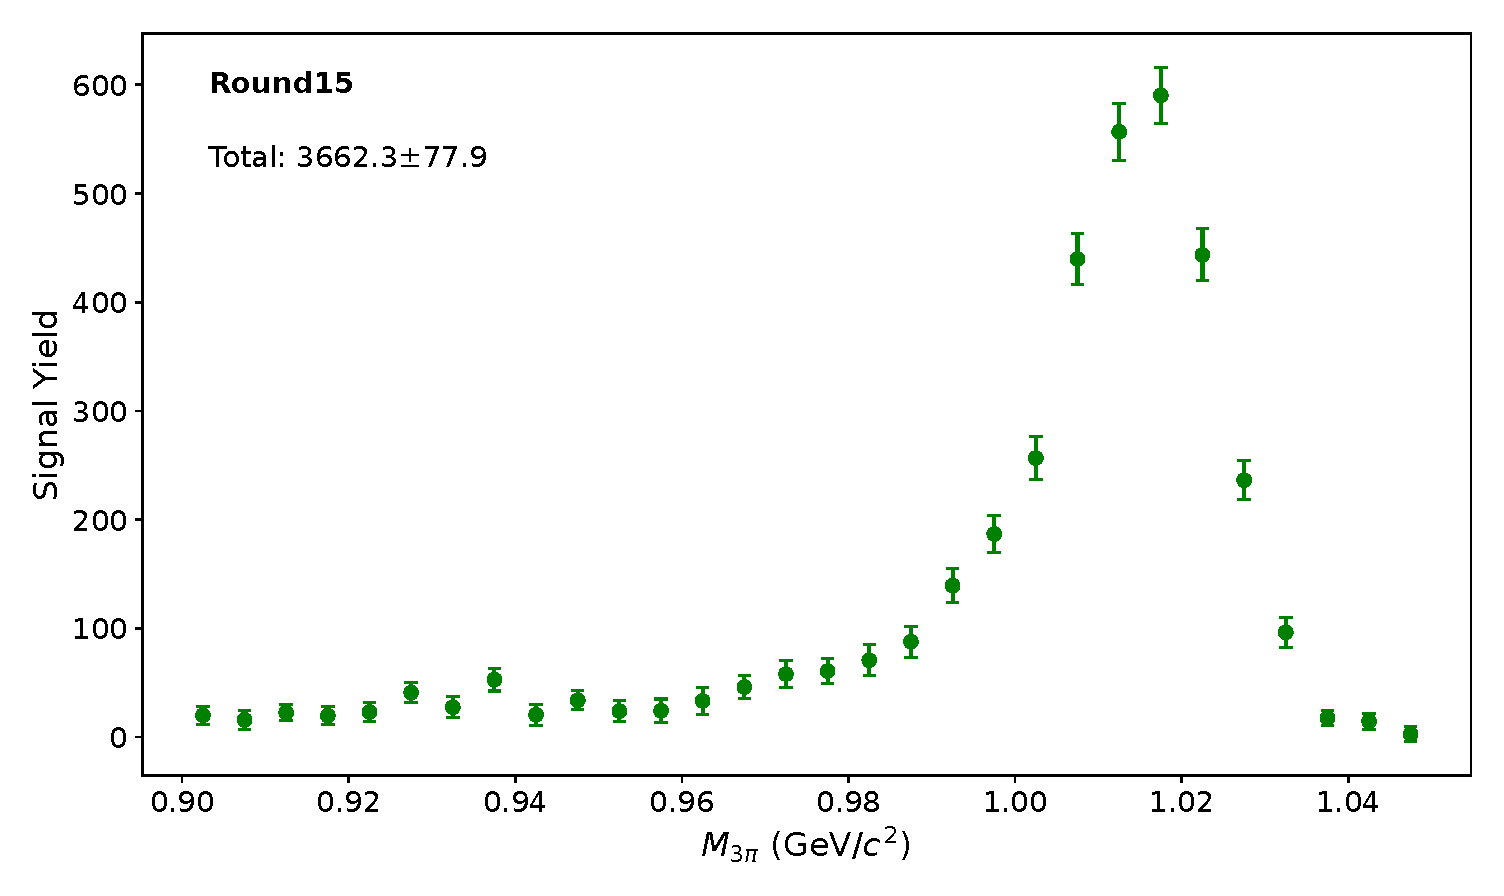
\includegraphics[width=0.32\textwidth]{fig/yields_round15_region2.eps}
    \label{fig:yields_r15_region2}
}\hfill
\subfloat[Round 15, $\omega^{\prime}/\omega^{\prime\prime}$ region]{
    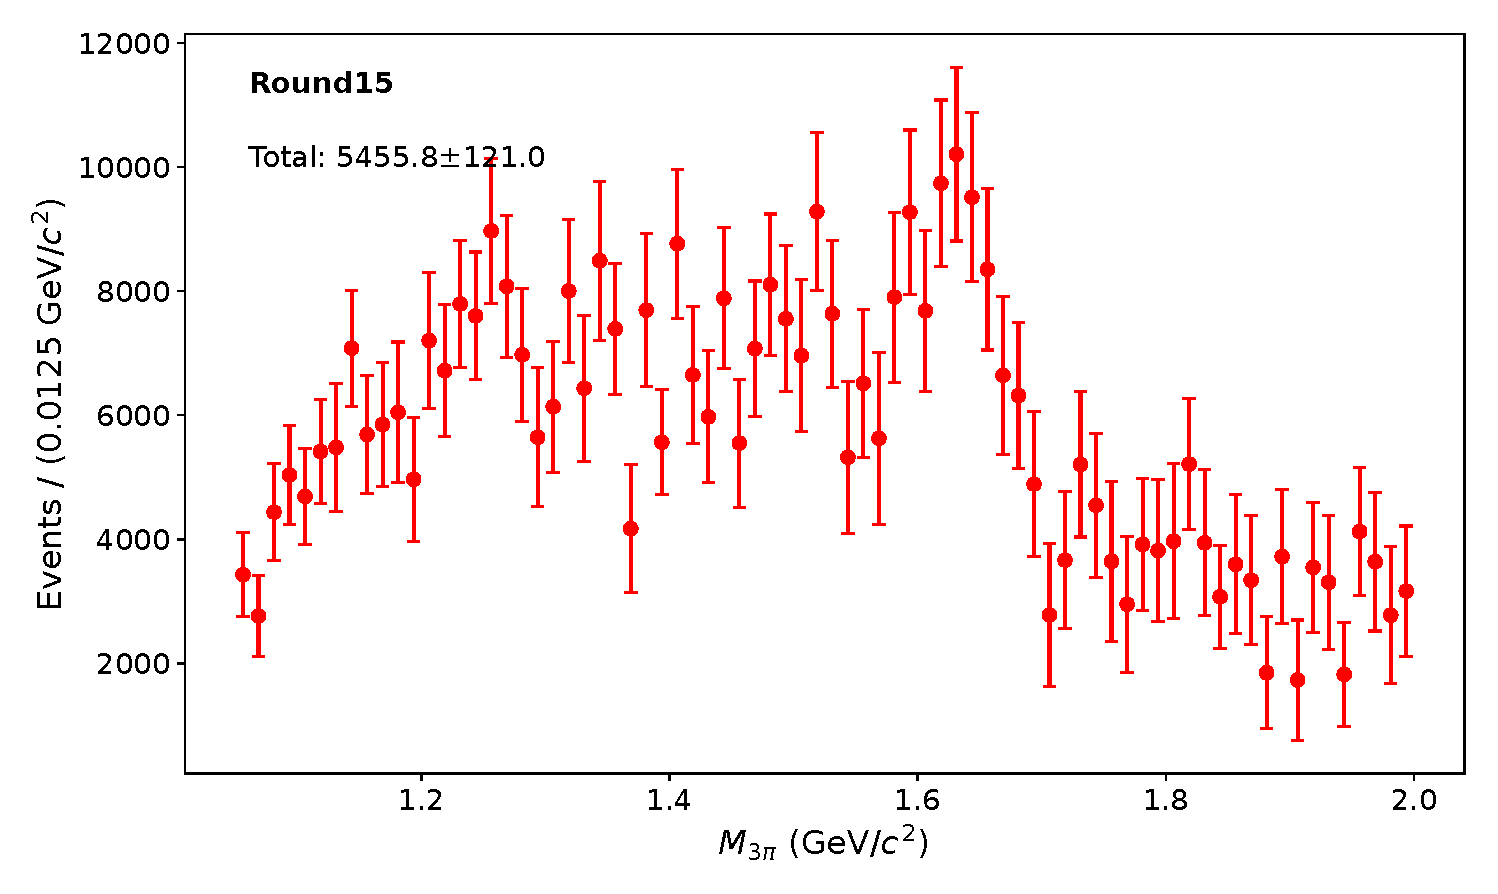
\includegraphics[width=0.32\textwidth]{fig/yields_round15_region3.eps}
    \label{fig:yields_r15_region3}
}

\vspace{0.5\baselineskip}

% === Row 3: Round 16 ===
\subfloat[Round 16, $\omega(782)$ region]{
    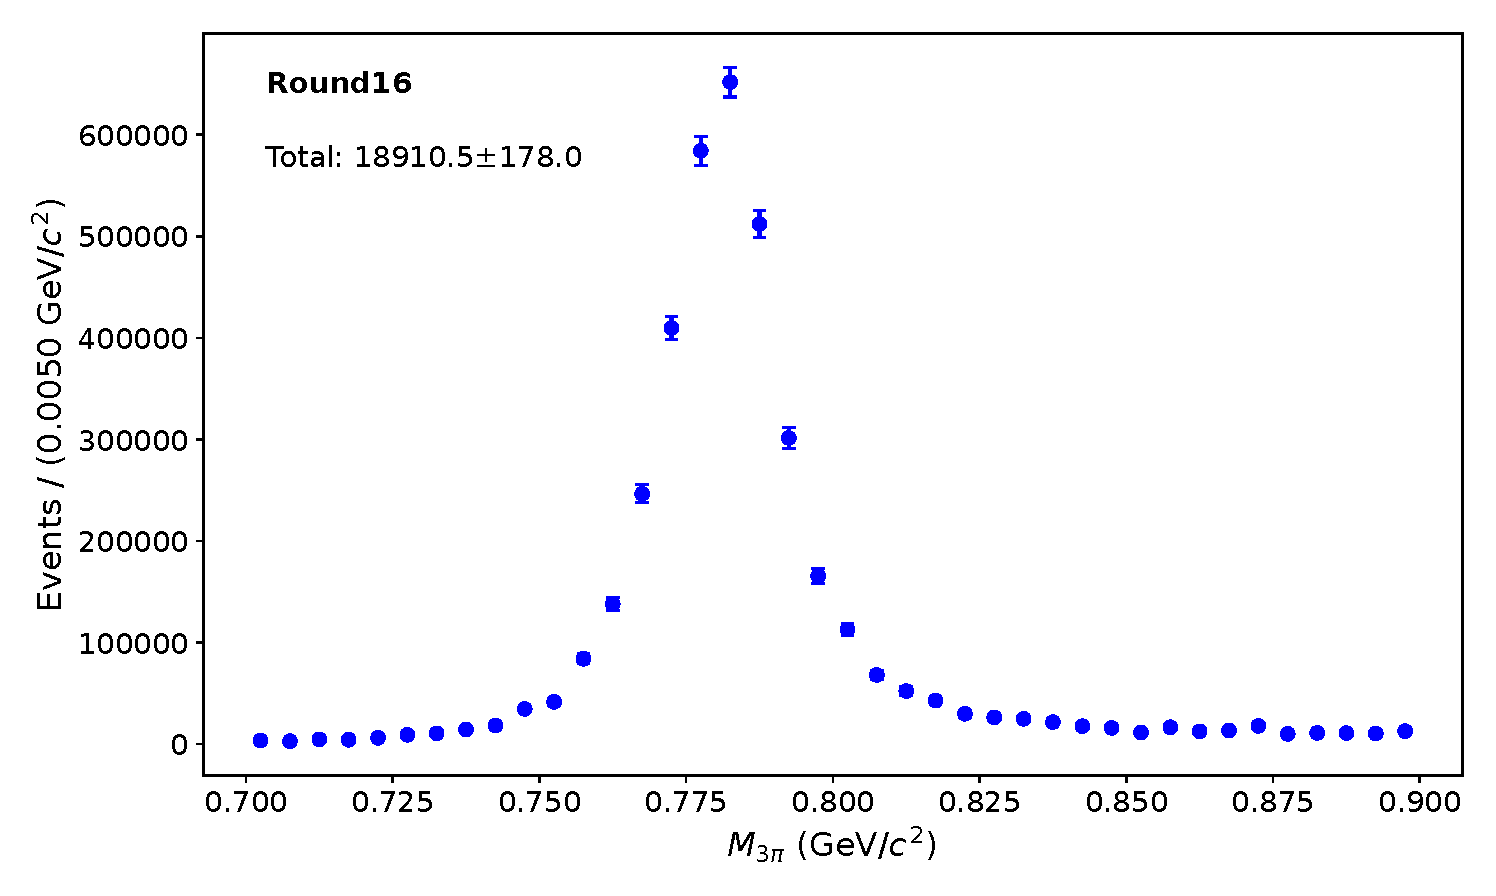
\includegraphics[width=0.32\textwidth]{fig/yields_round16_region1.eps}
    \label{fig:yields_r16_region1}
}\hfill
\subfloat[Round 16, $\phi(1020)$ region]{
    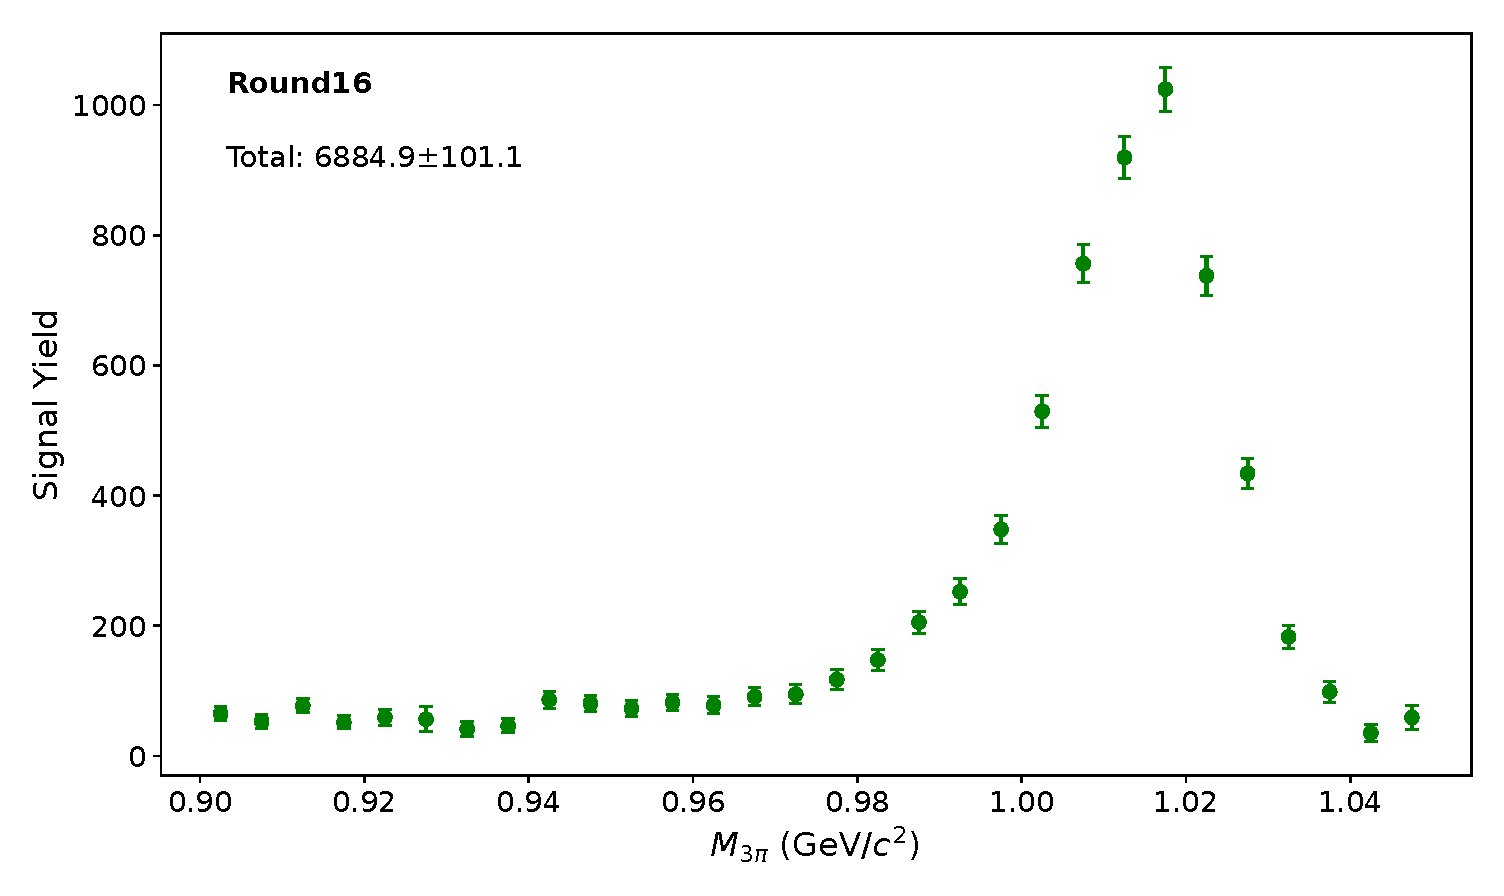
\includegraphics[width=0.32\textwidth]{fig/yields_round16_region2.eps}
    \label{fig:yields_r16_region2}
}\hfill
\subfloat[Round 16, $\omega^{\prime}/\omega^{\prime\prime}$ region]{
    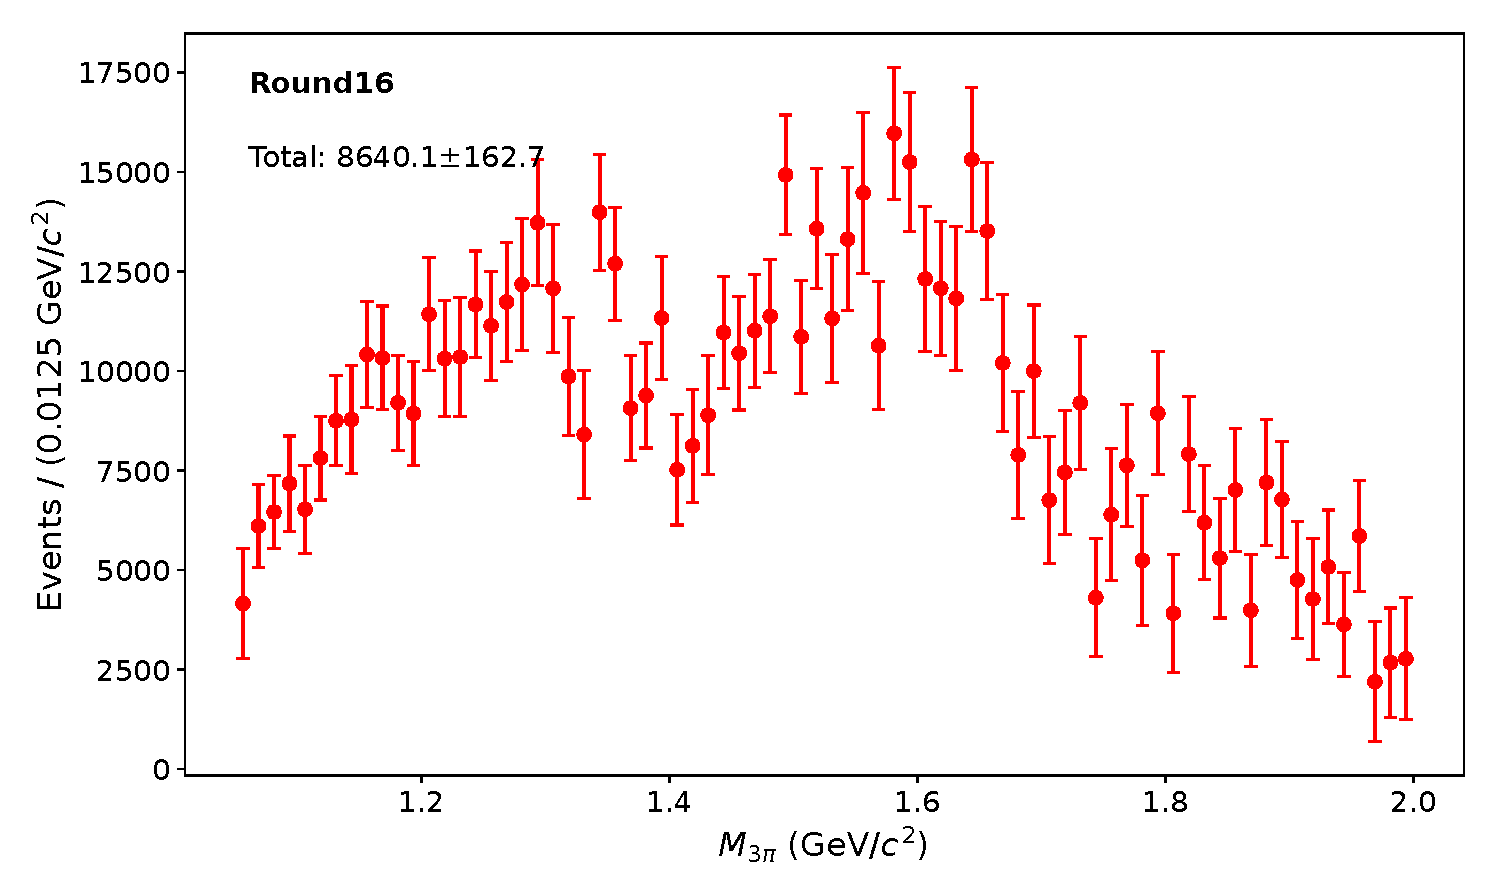
\includegraphics[width=0.32\textwidth]{fig/yields_round16_region3.eps}
    \label{fig:yields_r16_region3}
}

\vspace{0.5\baselineskip}

% === Row 4: Round 17 ===
\subfloat[Round 17, $\omega(782)$ region]{
    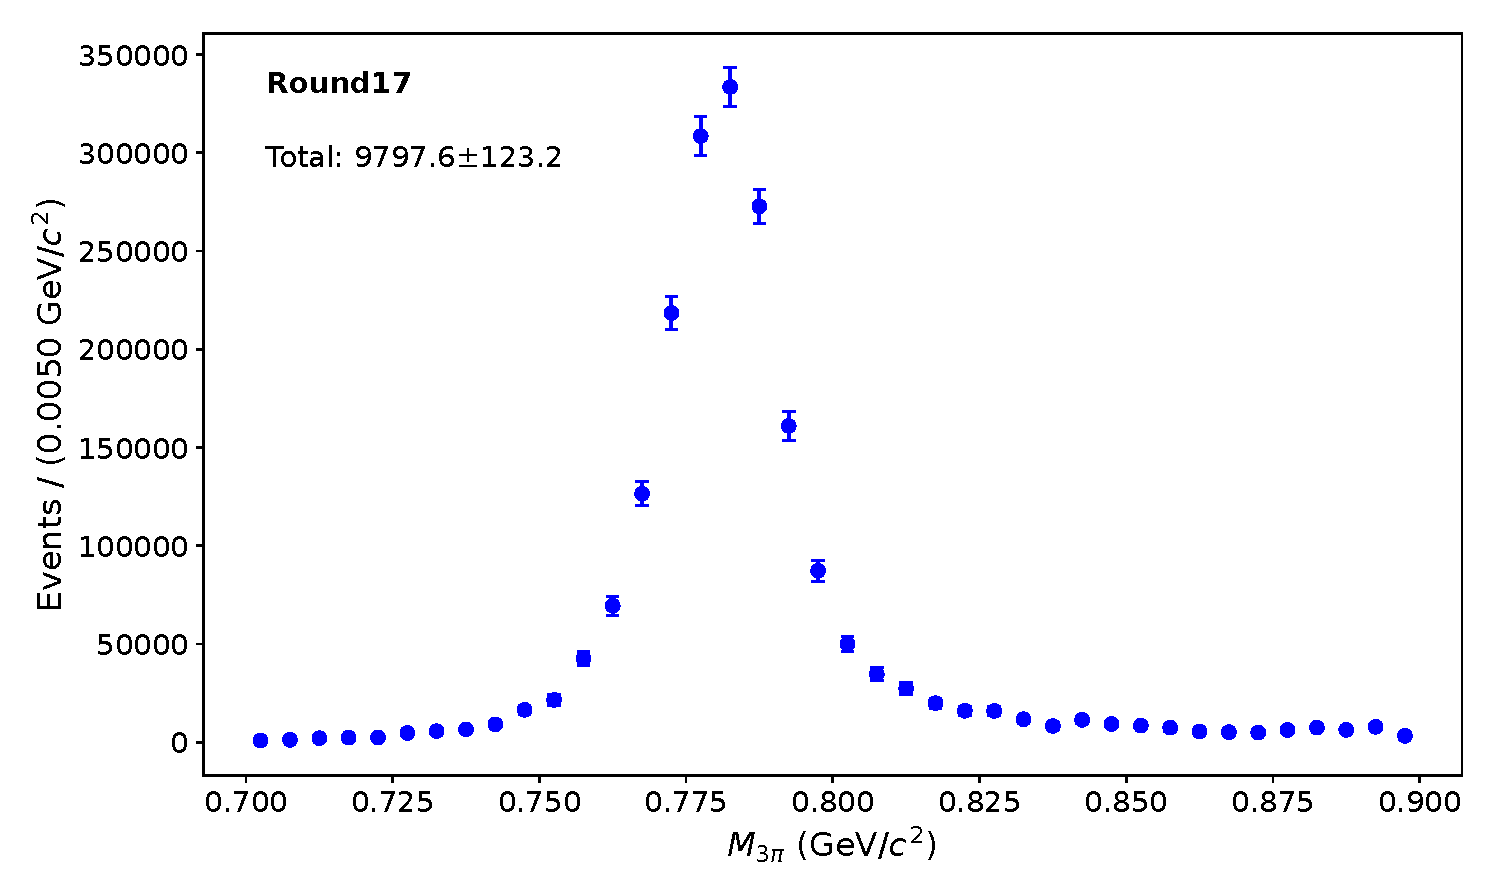
\includegraphics[width=0.32\textwidth]{fig/yields_round17_region1.eps}
    \label{fig:yields_r17_region1}
}\hfill
\subfloat[Round 17, $\phi(1020)$ region]{
    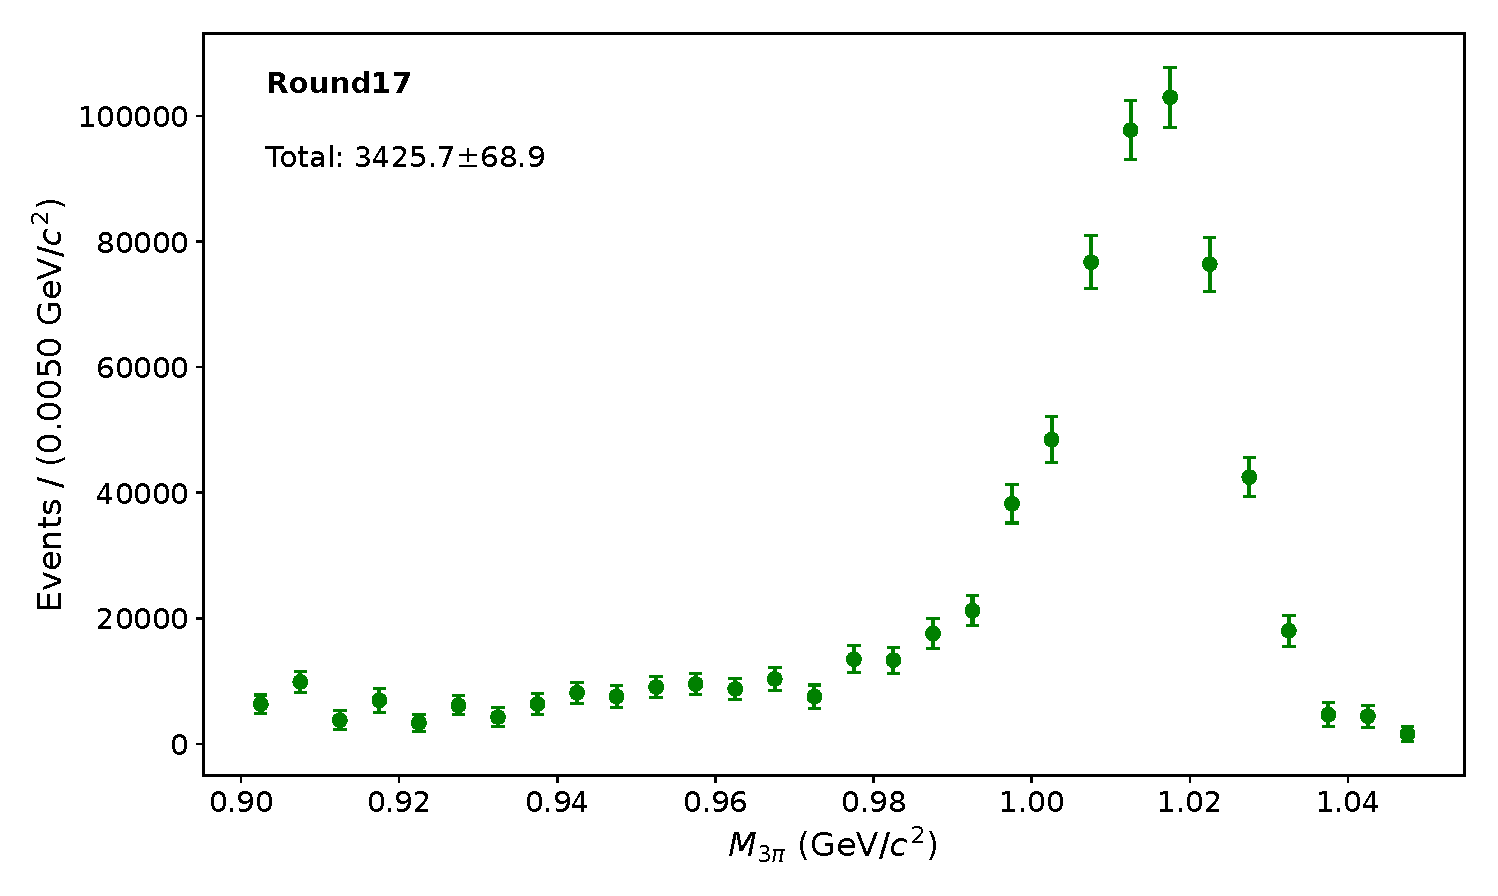
\includegraphics[width=0.32\textwidth]{fig/yields_round17_region2.eps}
    \label{fig:yields_r17_region2}
}\hfill
\subfloat[Round 17, $\omega^{\prime}/\omega^{\prime\prime}$ region]{
    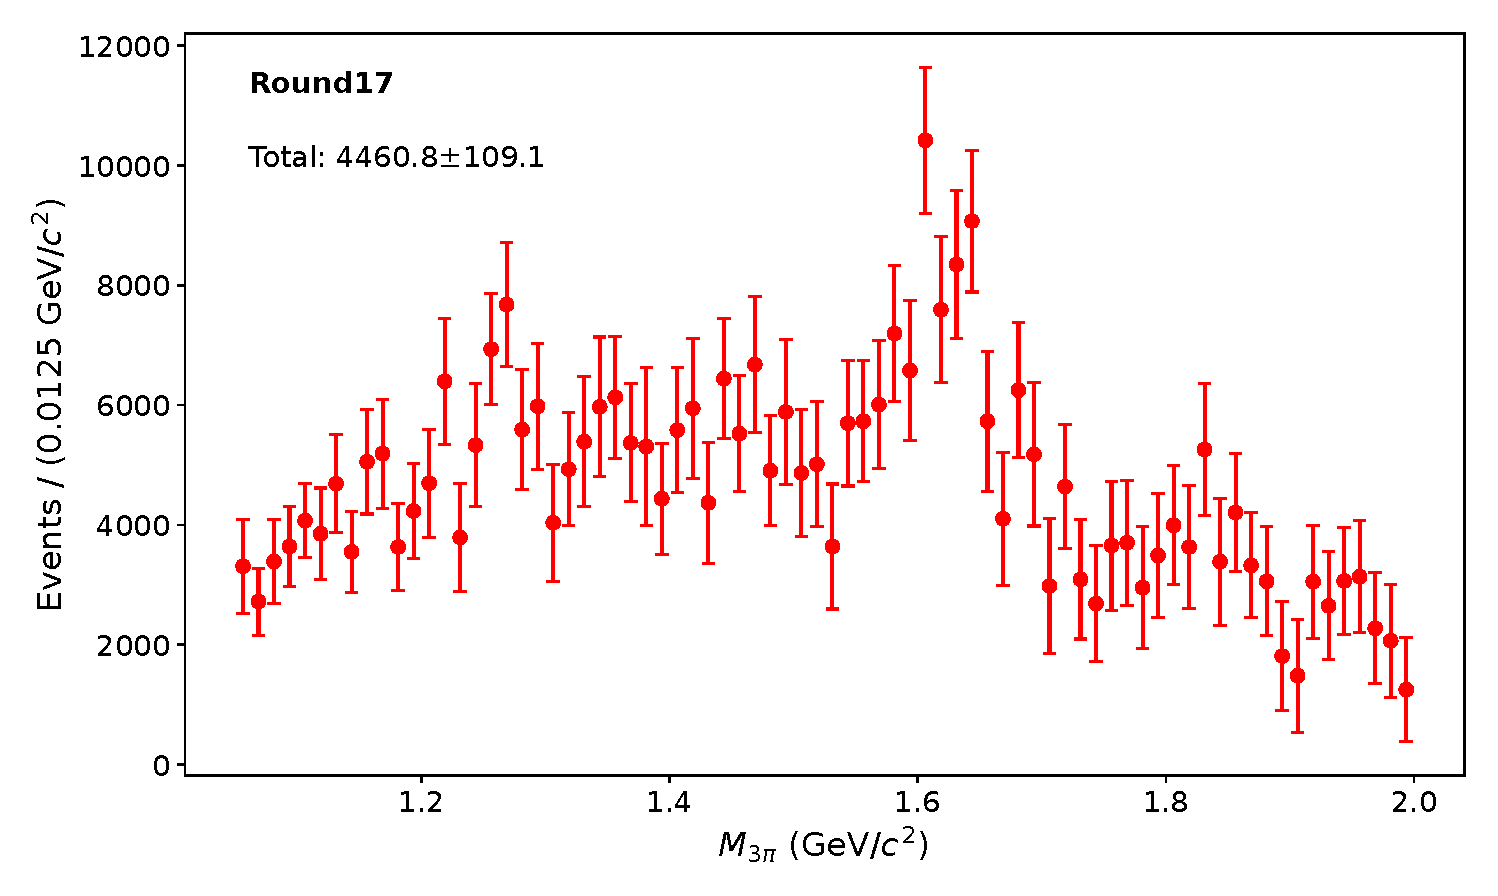
\includegraphics[width=0.32\textwidth]{fig/yields_round17_region3.eps}
    \label{fig:yields_r17_region3}
}

\caption{Extracted signal yields as a function of $M_{3\pi}$ for the three mass regions, shown separately for four data-taking periods. Each row corresponds to a different round: (a)--(c) Round~03/04, (d)--(f) Round~15, (g)--(i) Round~16, and (j)--(l) Round~17. The three columns represent different $3\pi$ invariant mass regions: $\omega(782)$ region (left), $\phi(1020)$ region (center), and higher-mass $\omega^{\prime}/\omega^{\prime\prime}$ region (right). Error bars represent the statistical uncertainties from the fits.}
\label{fig:signal_yields}
\end{figure}

% The signal yields obtained from this fitting procedure provide the foundation for calculating the Born cross section for $e^{+}e^{-} \to \pi^{+}\pi^{-}\pi^{0}$ as a function of $M_{3\pi}$. After applying efficiency corrections, unfolding for resolution effects, and subtracting residual background contributions, the cross section will be determined and compared with previous measurements and theoretical predictions.

% The fit results for the same three representative $M_{3\pi}$ bins are shown in Fig.~\ref{fig:fit_result_examples}, demonstrating the performance of the fitting procedure.

% \begin{figure}[htbp]
%     \centering
%     \subfloat[Low $M_{3\pi}$ bin fit result]{
%         \includegraphics[width=0.32\textwidth]{fig/fit_result_bin_low.eps}
%         \label{fig:fit_low}
%     }
%     \hfill
%     \subfloat[Medium $M_{3\pi}$ bin fit result]{
%         \includegraphics[width=0.32\textwidth]{fig/fit_result_bin_medium.eps}
%         \label{fig:fit_medium}
%     }
%     \hfill
%     \subfloat[High $M_{3\pi}$ bin fit result]{
%         \includegraphics[width=0.32\textwidth]{fig/fit_result_bin_high.eps}
%         \label{fig:fit_high}
%     }
%     \caption{Fit results to the $U_{\text{miss}}$ distributions for the same three representative $M_{3\pi}$ bins as in Fig.~\ref{fig:inclusiveMC_umiss_examples}. Data points are shown with error bars, while the solid black line represents the total fit. The individual components are displayed with the same color scheme as in Fig.~\ref{fig:inclusiveMC_umiss_examples}.}
%     \label{fig:fit_result_examples}
% \end{figure}

% The signal yields extracted from the fits in all $M_{3\pi}$ bins are then combined to form the signal mass spectra for each of the three regions. These spectra, showing the signal yield as a function of $M_{3\pi}$, are presented in Fig.~\ref{fig:signal_yield_spectra}.

% \begin{figure}[htbp]
%     \centering
%     \subfloat[$\omega(782)$ region]{
%         \includegraphics[width=0.32\textwidth]{fig/signal_yield_omega.eps}
%         \label{fig:signal_yield_omega}
%     }
%     \hfill
%     \subfloat[$\phi(1020)$ region]{
%         \includegraphics[width=0.32\textwidth]{fig/signal_yield_phi.eps}
%         \label{fig:signal_yield_phi}
%     }
%     \hfill
%     \subfloat[$\omega^{\prime}/\omega^{\prime\prime}$ region]{
%         \includegraphics[width=0.32\textwidth]{fig/signal_yield_omegaprime.eps}
%         \label{fig:signal_yield_omegaprime}
%     }
%     \caption{Extracted signal yields as a function of $M_{3\pi}$ for (a) the $\omega(782)$ region, (b) the $\phi(1020)$ region, and (c) the $\omega^{\prime}/\omega^{\prime\prime}$ region. The yields are obtained from the extended unbinned maximum-likelihood fits to the $U_{\text{miss}}$ distributions in each $M_{3\pi}$ bin.}
%     \label{fig:signal_yield_spectra}
% \end{figure}
    \clearpage
\section{Unfolding}
\label{sec:unfolding}
to fill
    \clearpage
\section{Efficiency correction}
\label{sec:eff_corr}
to fill
    \clearpage
\section{Systematic uncertainties}
\label{sec:sysU}
to fill
    \clearpage
\section{Summary}
\label{sec:summary}
\subsection{Calculation of cross sections}
From the unfolding procedure described in the previous section, we obtain the unfolded $M_{3\pi}$ mass spectrum $\left( \frac{dN}{dm} \right)^{\text{unfold}}$ for each data-taking period. 
For practical analysis, we work in discrete mass bins. Let $\left( \frac{dN}{dm} \right)^{\text{unfold}}_i$ denote the unfolded yield in the $i$-th mass bin, and $\Delta L_i = \int_{m_i}^{m_{i+1}} \frac{dL}{dm} dm$ denote the integrated luminosity in that bin. The dressed cross section $\sigma_{3\pi}^{\text{dress}}(m)$ is then obtained by:
\begin{equation}
    \sigma_i^{\text{dress}} = \frac{\left( \frac{dN}{dm} \right)^{\text{unfold}}_i}{\Delta L_i \cdot \mathcal{B}(\pi^{0} \to \gamma\gamma)}
    \label{eq:dressed_cross_section}
\end{equation}
where $\mathcal{B}(\pi^{0} \to \gamma\gamma) = (98.823 \pm 0.034)\%$ is the branching fraction of $\pi^{0} \to \gamma\gamma$ as quoted by the Particle Data Group (PDG)~\cite{PDG2024}. The complete formula for calculating $\frac{dL}{dm}$ is provided in Sec.~\ref{sec:bkg_stu}.

The unfolding procedure yields not only the unfolded spectrum $\left( \frac{dN}{dm} \right)^{\text{unfold}}_i$ but also its covariance matrix $\mathbf{C}$, which fully describes the uncertainties and correlations of $\left( \frac{dN}{dm} \right)^{\text{unfold}}_i$. However, additional uncertainties arise from the luminosity measurement and the $\pi^0$ branching fraction. These must be propagated to the dressed cross section $\boldsymbol{\sigma}^{\text{dress}}$.

The integrated luminosity per bin $\Delta L_i$ is not a measured quantity but is calculated from the total integrated luminosity $L_{\text{total}}$ via $\Delta L_i = f_i \cdot L_{\text{total}}$, where $f_i = \frac{1}{L_{\text{total}}} \int_{m_i}^{m_{i+1}} \frac{d\mathcal{L}}{dm} dm$ is the theoretical shape factor determined from QED, considered to have negligible uncertainty. The total luminosity $L_{\text{total}}$ is measured with a relative uncertainty $\delta_L = \sigma_L / L_{\text{total}}$. For the present analysis, $\delta_L = 19.0 / 4995 \approx 0.38\%$. The luminosity uncertainty affects all mass bins in a {\it fully correlated} manner: if the measured total luminosity is overestimated by $1\%$, all $\Delta L_i$ are overestimated by $1\%$, and consequently all $\sigma_i^{\text{dress}}$ are underestimated by $1\%$. This full correlation is a crucial property of normalization uncertainties.

Similarly, the $\pi^0 \to \gamma\gamma$ branching fraction $\mathcal{B}$ is known from PDG with a relative uncertainty $\delta_{\mathcal{B}} = \sigma_{\mathcal{B}} / \mathcal{B} \approx 0.034\%$. This uncertainty is also {\it fully correlated} across all mass bins, since the same branching fraction is used to normalize every bin.

The total covariance matrix of the dressed cross section combines three independent sources of uncertainty: the statistical and systematic uncertainties from the unfolding (encoded in $\mathbf{C}$), the luminosity uncertainty, and the $\pi^0$ branching fraction uncertainty. These sources are independent, so their covariance matrices add linearly. The propagation proceeds as follows.

First, the unfolded spectrum covariance is propagated through division by $\Delta L_i \cdot \mathcal{B}$. With $\sigma_i^{\text{dress}} = \left( \frac{dN}{dm} \right)^{\text{unfold}}_i / (\Delta L_i \cdot \mathcal{B})$, the Jacobian matrix is diagonal with elements $\partial \sigma_i^{\text{dress}} / \partial \left( \frac{dN}{dm} \right)^{\text{unfold}}_j = \delta_{ij} / (\Delta L_i \cdot \mathcal{B})$. Therefore:
\begin{equation}
    \left[\mathbf{C}_{\sigma}^{\text{(unfold)}}\right]_{ij} = \frac{\left[\mathbf{C}\right]_{ij}}{(\Delta L_i \cdot \mathcal{B})(\Delta L_j \cdot \mathcal{B})} = \frac{\left[\mathbf{C}\right]_{ij}}{\Delta L_i \Delta L_j \mathcal{B}^2}
    \label{eq:unfold_covariance}
\end{equation}
or in matrix form $\mathbf{C}_{\sigma}^{\text{(unfold)}} = \mathbf{D} \cdot \mathbf{C} \cdot \mathbf{D}^T$, where $\mathbf{D} = \operatorname{diag}(1/(\Delta L_i \mathcal{B}))$.

Second, the luminosity uncertainty, being fully correlated, contributes a rank-1 covariance matrix:
\begin{equation}
    \left[\mathbf{C}_{\sigma}^{\text{(lumi)}}\right]_{ij} = \sigma_i^{\text{dress}} \cdot \sigma_j^{\text{dress}} \cdot \delta_L^2 = \delta_L^2 \cdot \boldsymbol{\sigma}^{\text{dress}} (\boldsymbol{\sigma}^{\text{dress}})^T
    \label{eq:lumi_covariance}
\end{equation}
The correlation coefficient between any two bins from this source is $\rho_{ij} = 1$, reflecting complete correlation.

Third, the $\pi^0$ branching fraction uncertainty, also fully correlated, contributes similarly:
\begin{equation}
    \left[\mathbf{C}_{\sigma}^{\text{(BR)}}\right]_{ij} = \sigma_i^{\text{dress}} \cdot \sigma_j^{\text{dress}} \cdot \delta_{\mathcal{B}}^2 = \delta_{\mathcal{B}}^2 \cdot \boldsymbol{\sigma}^{\text{dress}} (\boldsymbol{\sigma}^{\text{dress}})^T
    \label{eq:br_covariance}
\end{equation}

The total covariance matrix for the dressed cross section is then:
\begin{equation}
    \mathbf{C}_{\sigma}^{\text{(dress)}} = \mathbf{C}_{\sigma}^{\text{(unfold)}} + (\delta_L^2 + \delta_{\mathcal{B}}^2) \cdot \boldsymbol{\sigma}^{\text{dress}} (\boldsymbol{\sigma}^{\text{dress}})^T
    \label{eq:total_covariance}
\end{equation}

The total uncertainty for each bin is given by $\sigma_{\sigma_i^{\text{dress}}} = \sqrt{\left[\mathbf{C}_{\sigma}^{\text{(dress)}}\right]_{ii}}$. For a single bin, the relative uncertainty squares add quadratically:
\begin{equation}
    \left(\frac{\Delta \sigma_i^{\text{dress}}}{\sigma_i^{\text{dress}}}\right)^2 = \left(\frac{\Delta \left( \frac{dN}{dm} \right)^{\text{unfold}}_i}{\left( \frac{dN}{dm} \right)^{\text{unfold}}_i}\right)^2 + \delta_L^2 + \delta_{\mathcal{B}}^2
    \label{eq:relative_error_decomposition}
\end{equation}
where $\Delta \left( \frac{dN}{dm} \right)^{\text{unfold}}_i / \left( \frac{dN}{dm} \right)^{\text{unfold}}_i$ is the relative uncertainty from the unfolding. For the present analysis, $\delta_L \approx 0.38\%$ dominates over $\delta_{\mathcal{B}} \approx 0.034\%$, while the unfolding uncertainty varies with mass and is typically the largest contribution.

It is important to note that while the diagonal elements follow Eq.~\ref{eq:relative_error_decomposition}, the off-diagonal elements retain the correlation structures of each source. The luminosity and branching fraction uncertainties introduce 100\% correlations across all bins, while the unfolding covariance $\mathbf{C}$ contains the correlations determined by the unfolding procedure.

Using Eq.~\ref{eq:total_covariance}, we obtain four independent dressed cross section results $\sigma_{3\pi}^{\text{dress}}(m)$ corresponding to the four data-taking periods: Round~03/04, Round~15, Round~16, and Round~17. These results are presented in Fig.~\ref{fig:sigma_dress_results_all_rounds} along with their total uncertainties, which now properly include the luminosity and $\pi^0$ branching fraction contributions.

\begin{figure}[htbp]
    \centering

    % === Row 1: Round 03/04 ===
    \subfloat[Round 03/04, $\omega(782)$ region]{
        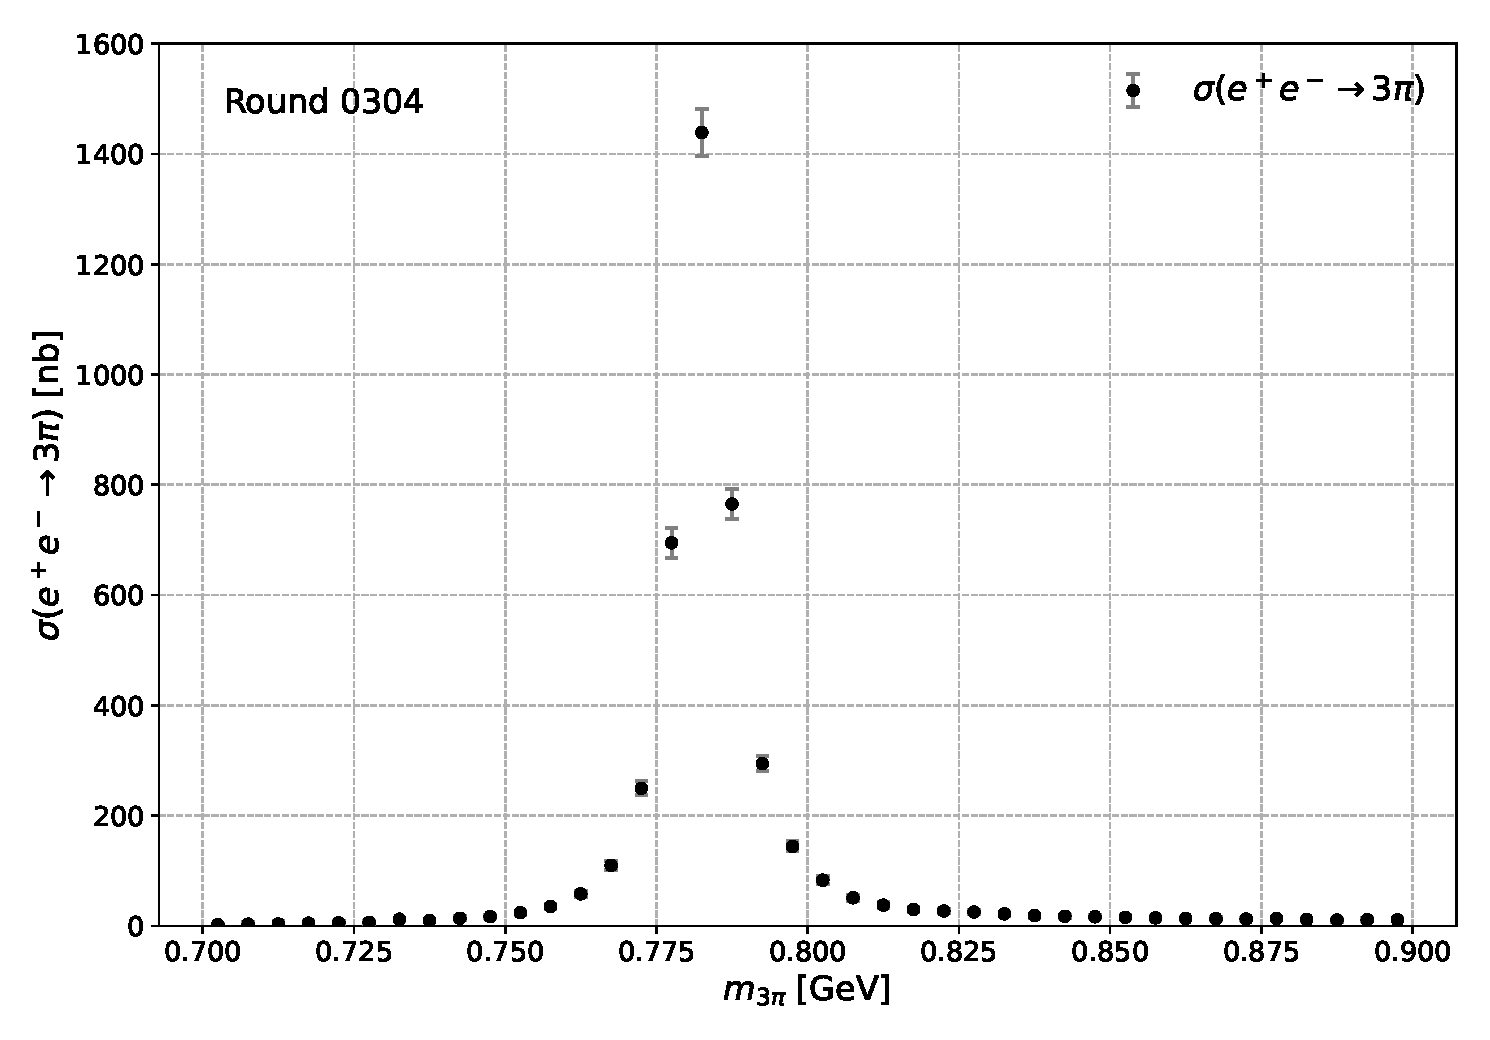
\includegraphics[width=0.32\textwidth]{fig/sigma_final_round0304_omega.eps}
        \label{fig:sigma_final_round0304_omega}
    }\hfill
    \subfloat[Round 03/04, $\phi(1020)$ region]{
        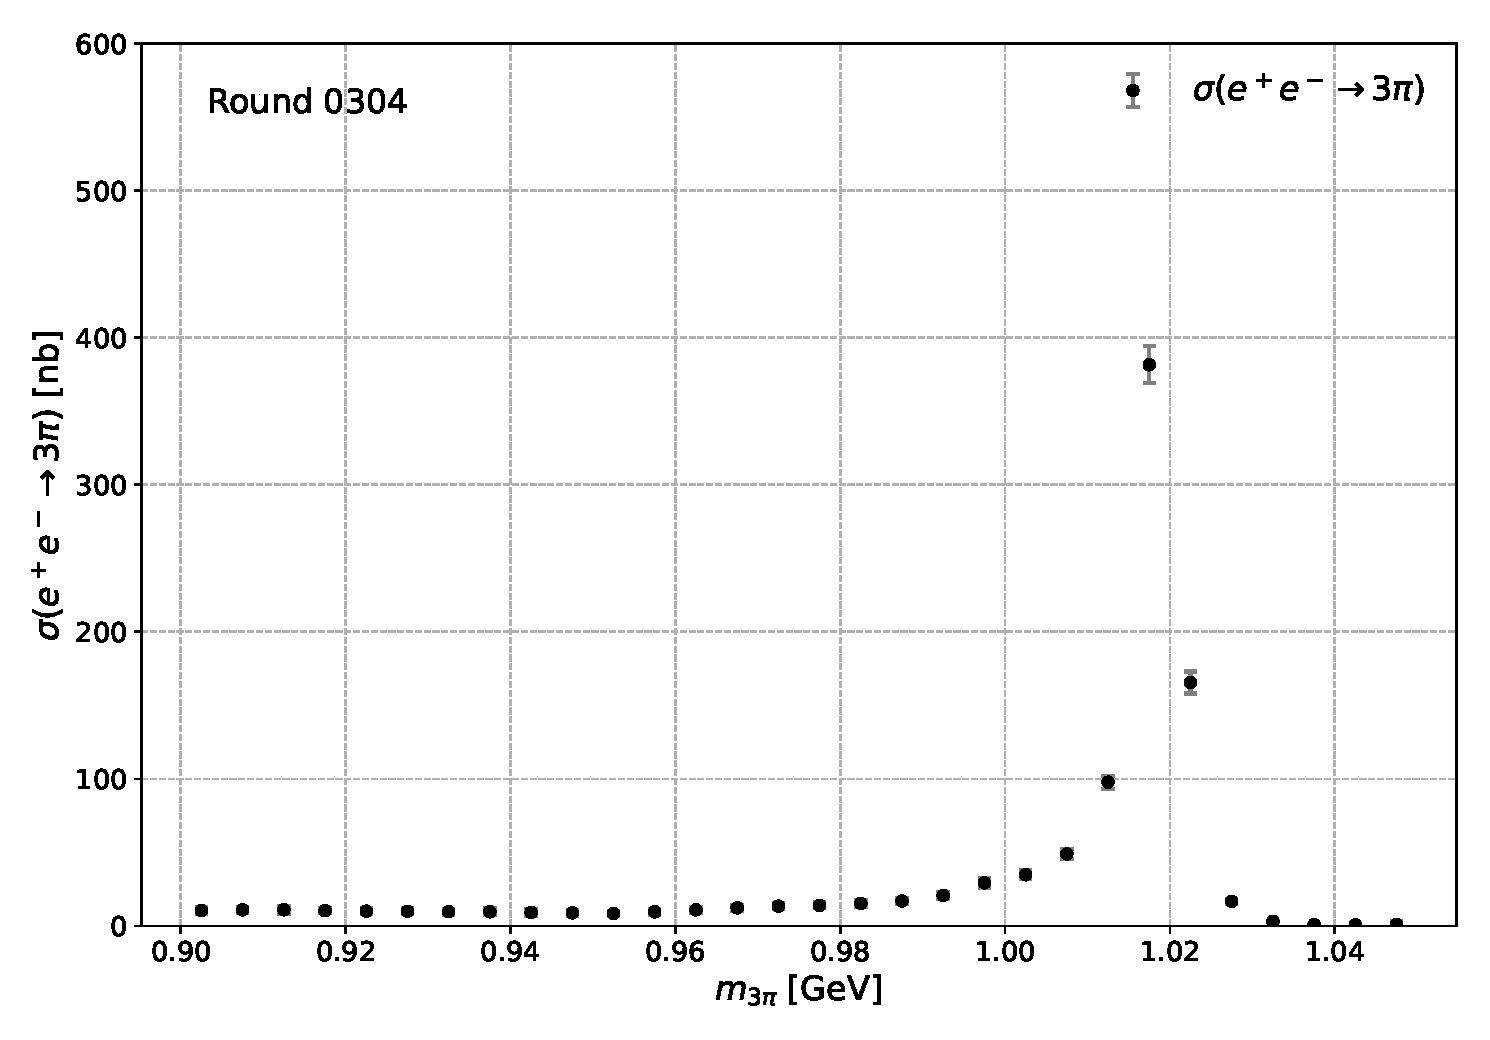
\includegraphics[width=0.32\textwidth]{fig/sigma_final_round0304_phi.eps}
        \label{fig:sigma_final_round0304_phi}
    }\hfill
    \subfloat[Round 03/04, $\omega^{\prime}/\omega^{\prime\prime}$ region]{
        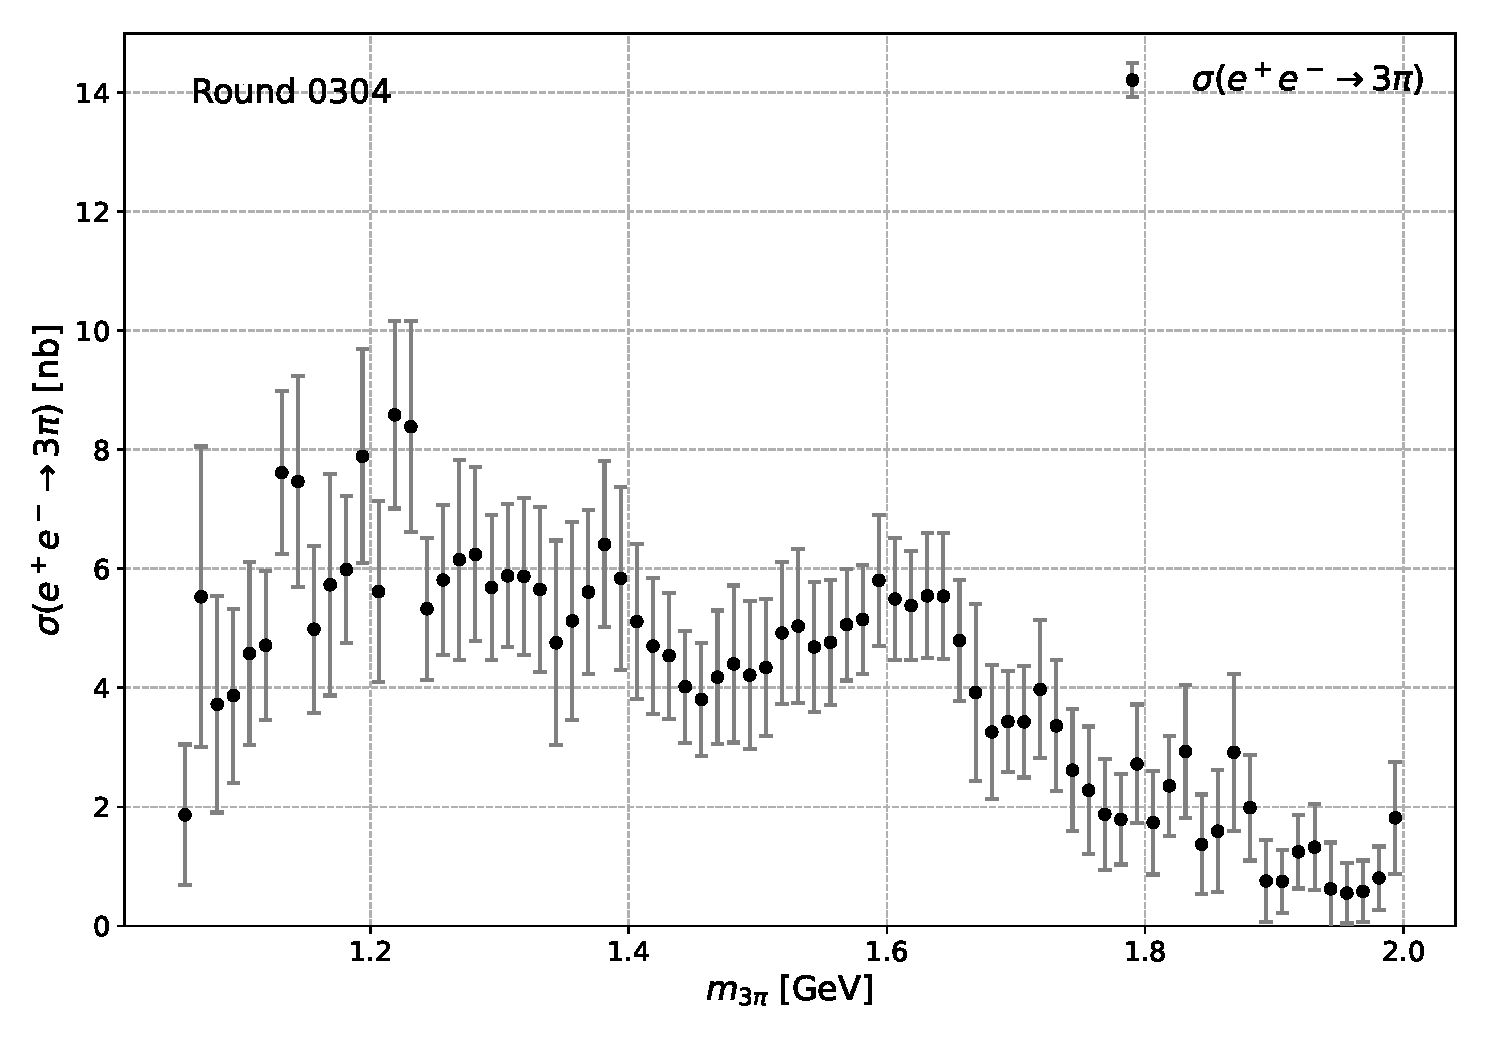
\includegraphics[width=0.32\textwidth]{fig/sigma_final_round0304_high.eps}
        \label{fig:sigma_final_round0304_high}
    }

    \vspace{0.5\baselineskip}

    % === Row 2: Round 15 ===
    \subfloat[Round 15, $\omega(782)$ region]{
        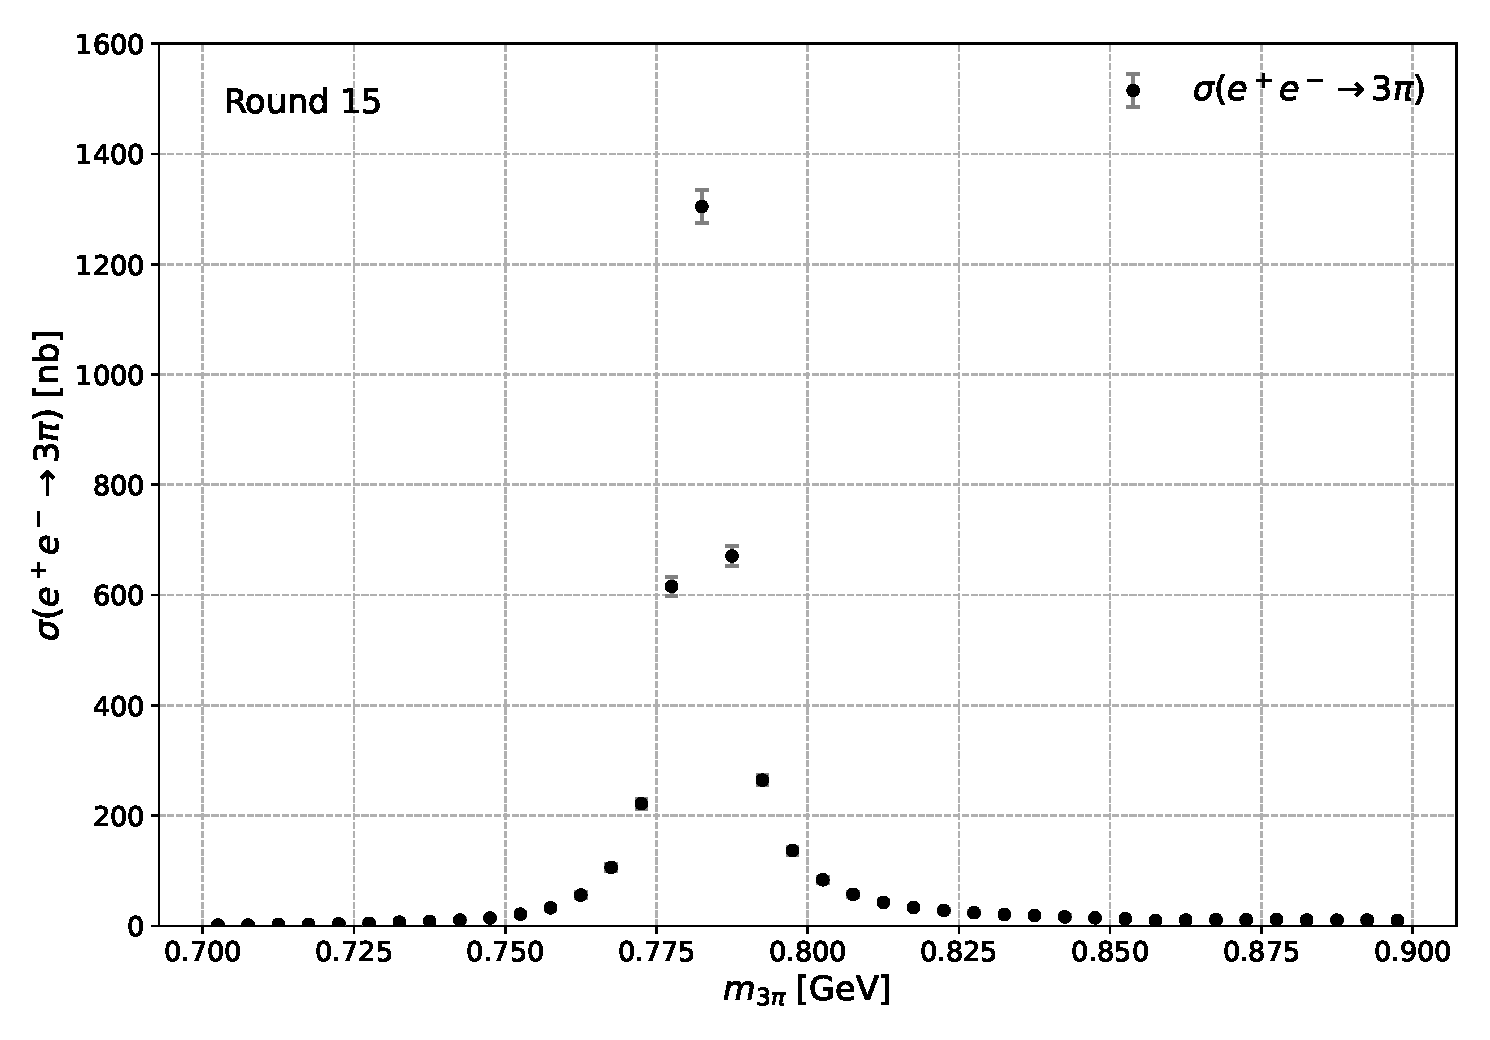
\includegraphics[width=0.32\textwidth]{fig/sigma_final_round15_omega.eps}
        \label{fig:sigma_final_round15_omega}
    }\hfill
    \subfloat[Round 15, $\phi(1020)$ region]{
        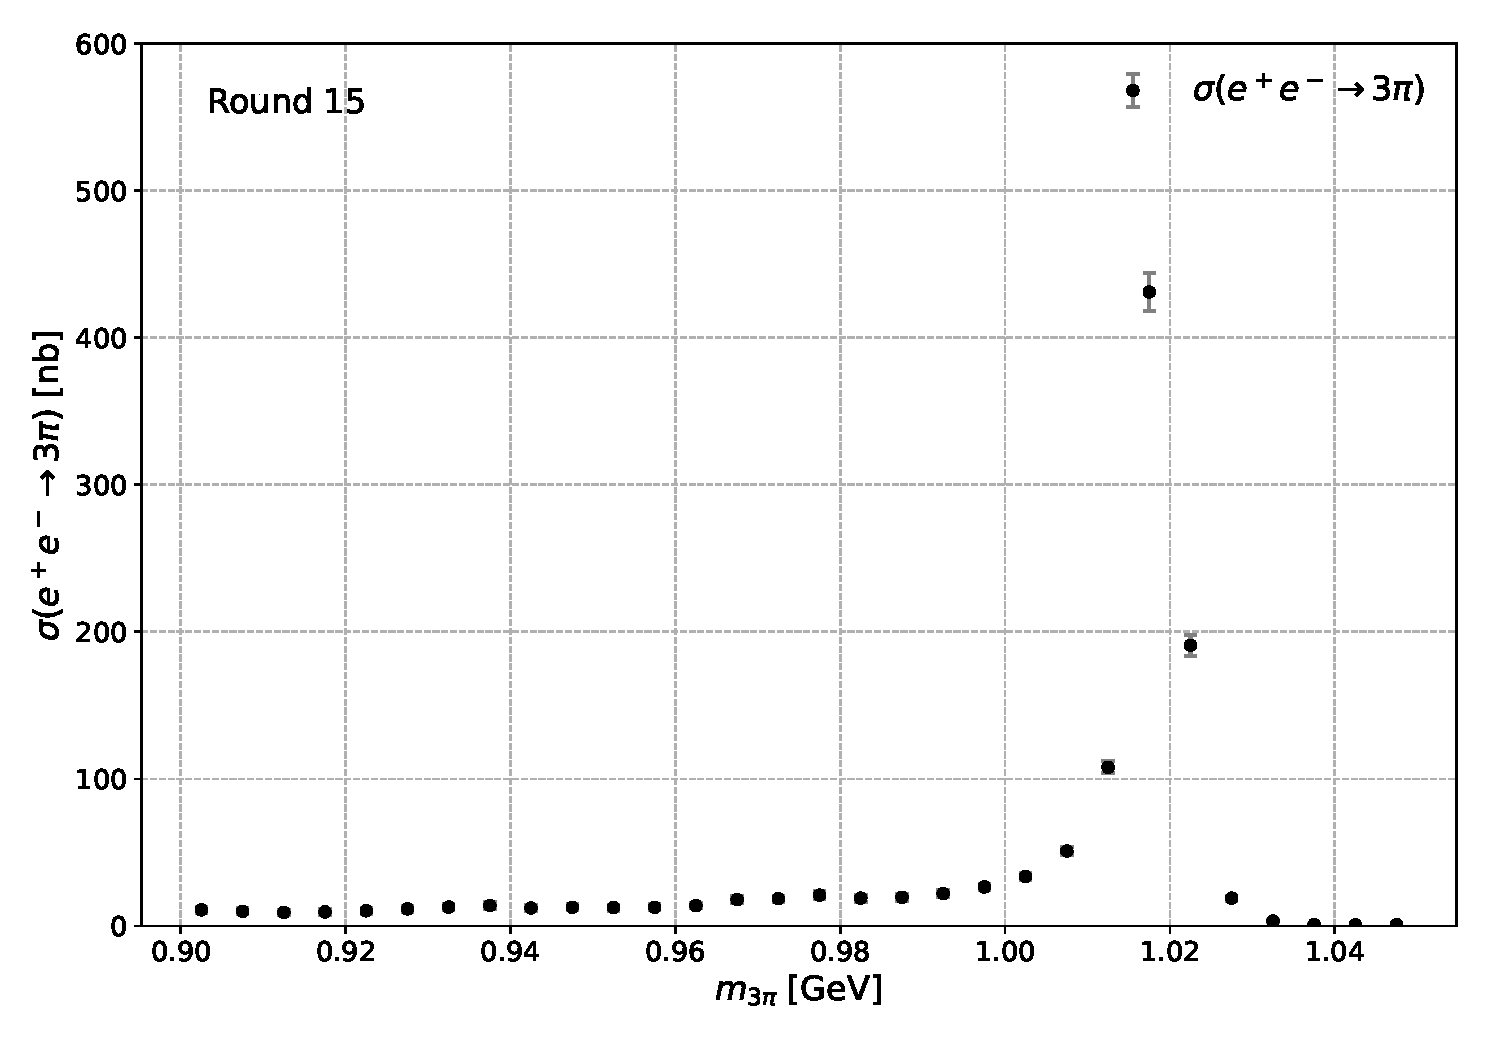
\includegraphics[width=0.32\textwidth]{fig/sigma_final_round15_phi.eps}
        \label{fig:sigma_final_round15_phi}
    }\hfill
    \subfloat[Round 15, $\omega^{\prime}/\omega^{\prime\prime}$ region]{
        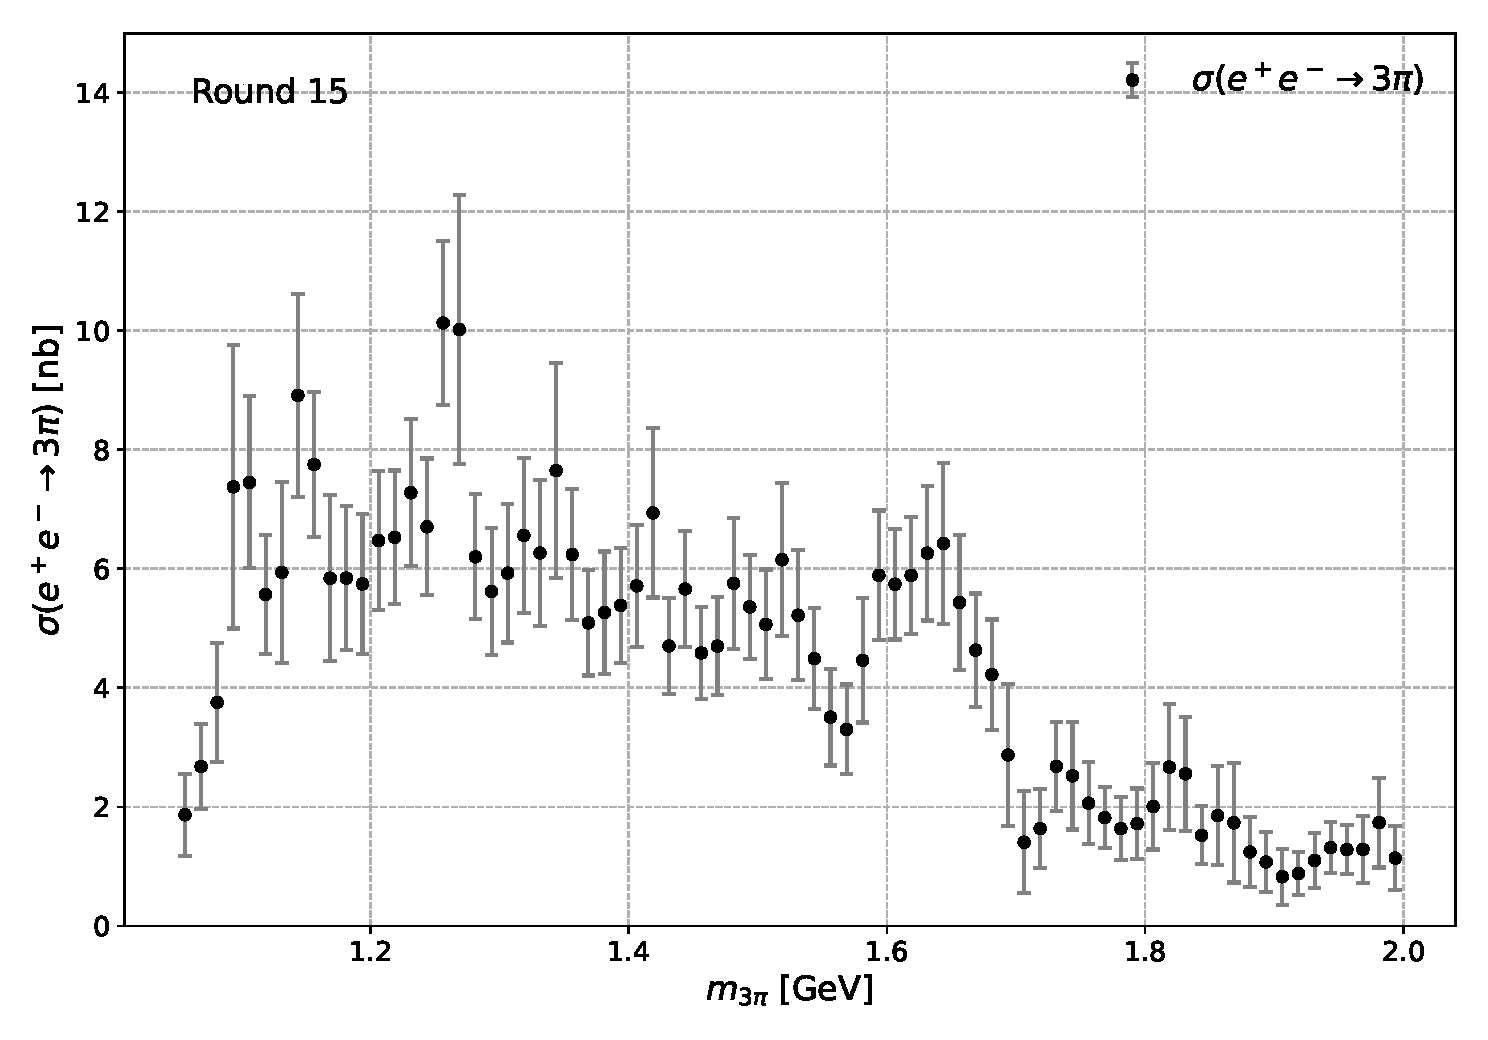
\includegraphics[width=0.32\textwidth]{fig/sigma_final_round15_high.eps}
        \label{fig:sigma_final_round15_high}
    }

    \vspace{0.5\baselineskip}

    % === Row 3: Round 16 ===
    \subfloat[Round 16, $\omega(782)$ region]{
        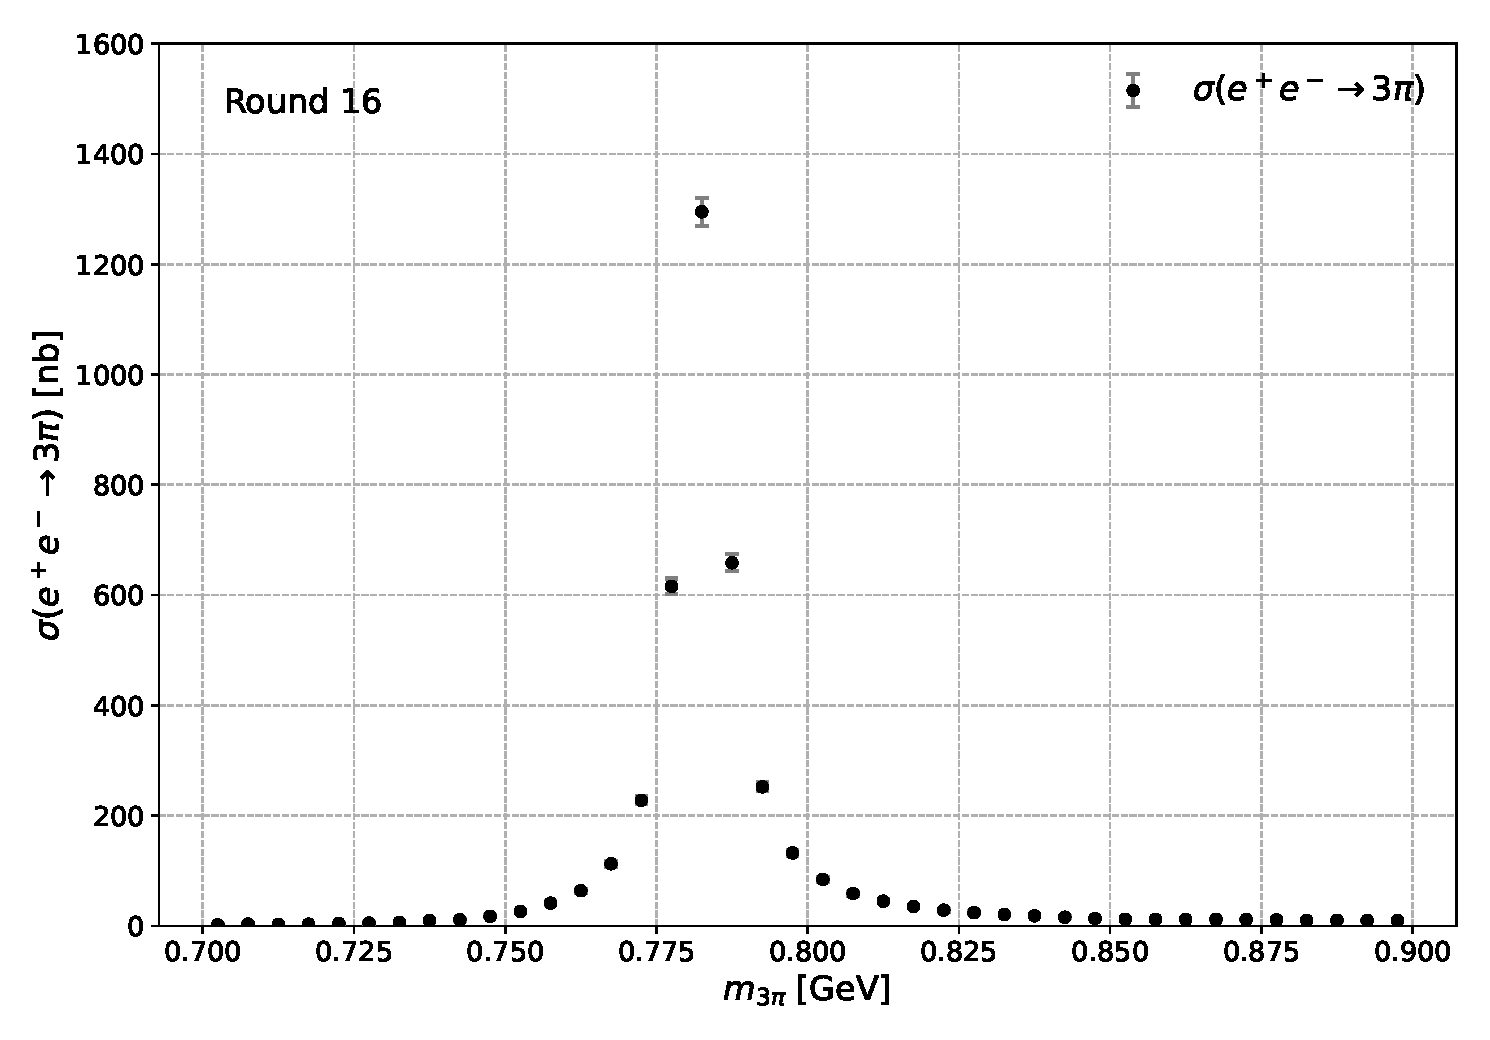
\includegraphics[width=0.32\textwidth]{fig/sigma_final_round16_omega.eps}
        \label{fig:sigma_final_round16_omega}
    }\hfill
    \subfloat[Round 16, $\phi(1020)$ region]{
        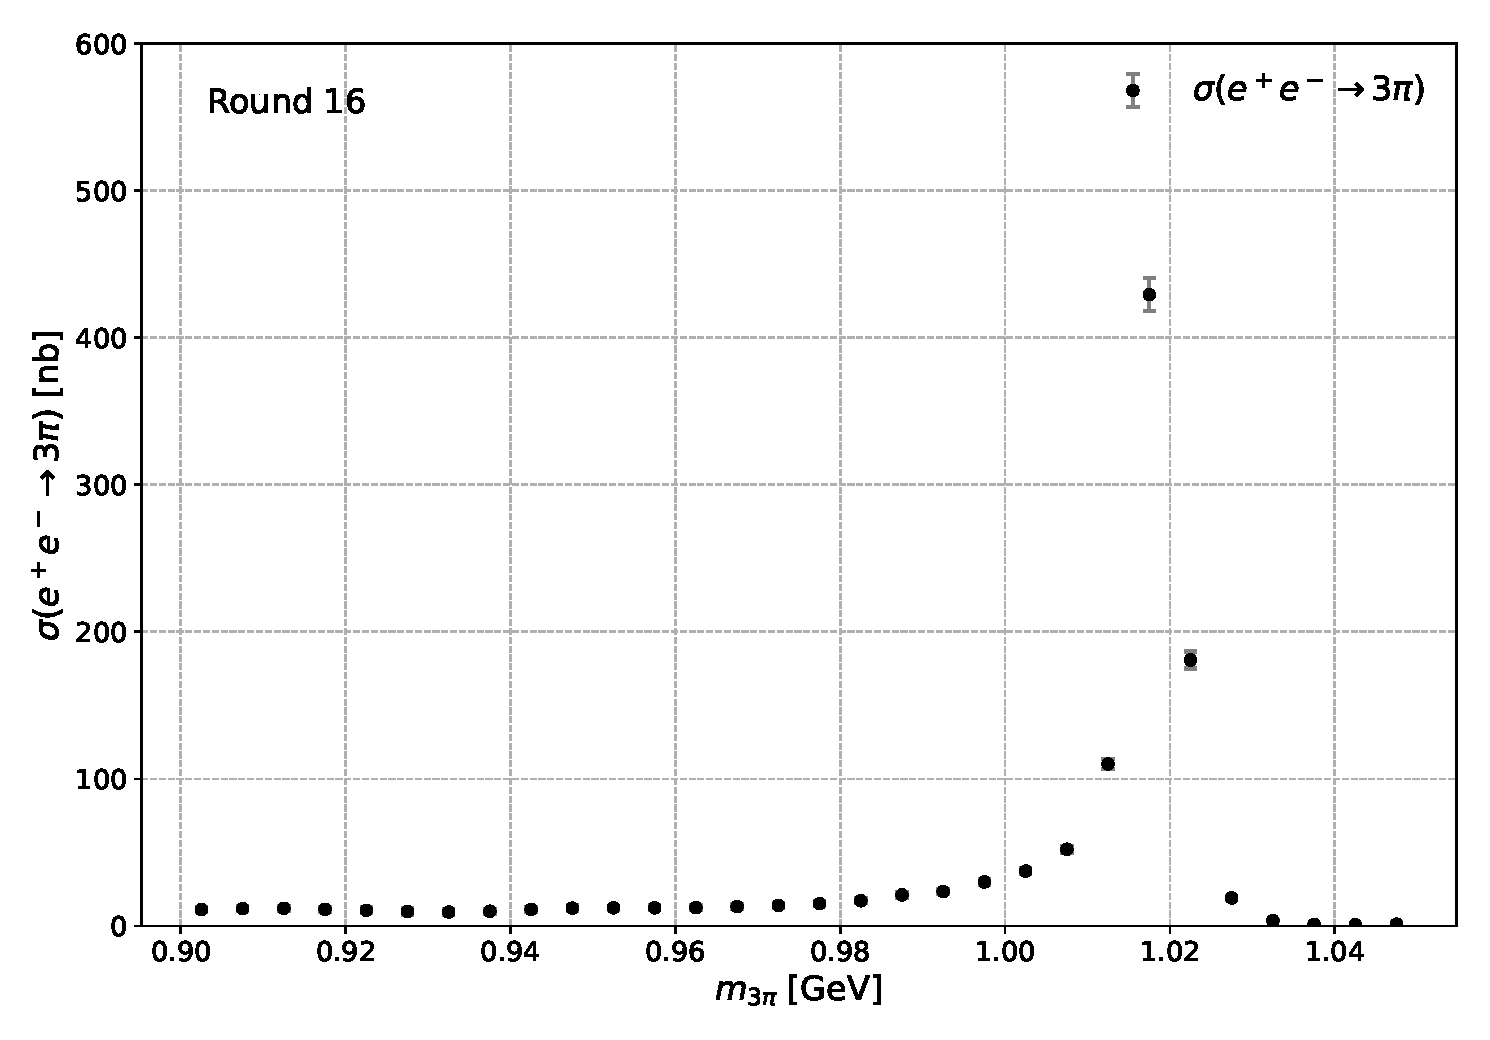
\includegraphics[width=0.32\textwidth]{fig/sigma_final_round16_phi.eps}
        \label{fig:sigma_final_round16_phi}
    }\hfill
    \subfloat[Round 16, $\omega^{\prime}/\omega^{\prime\prime}$ region]{
        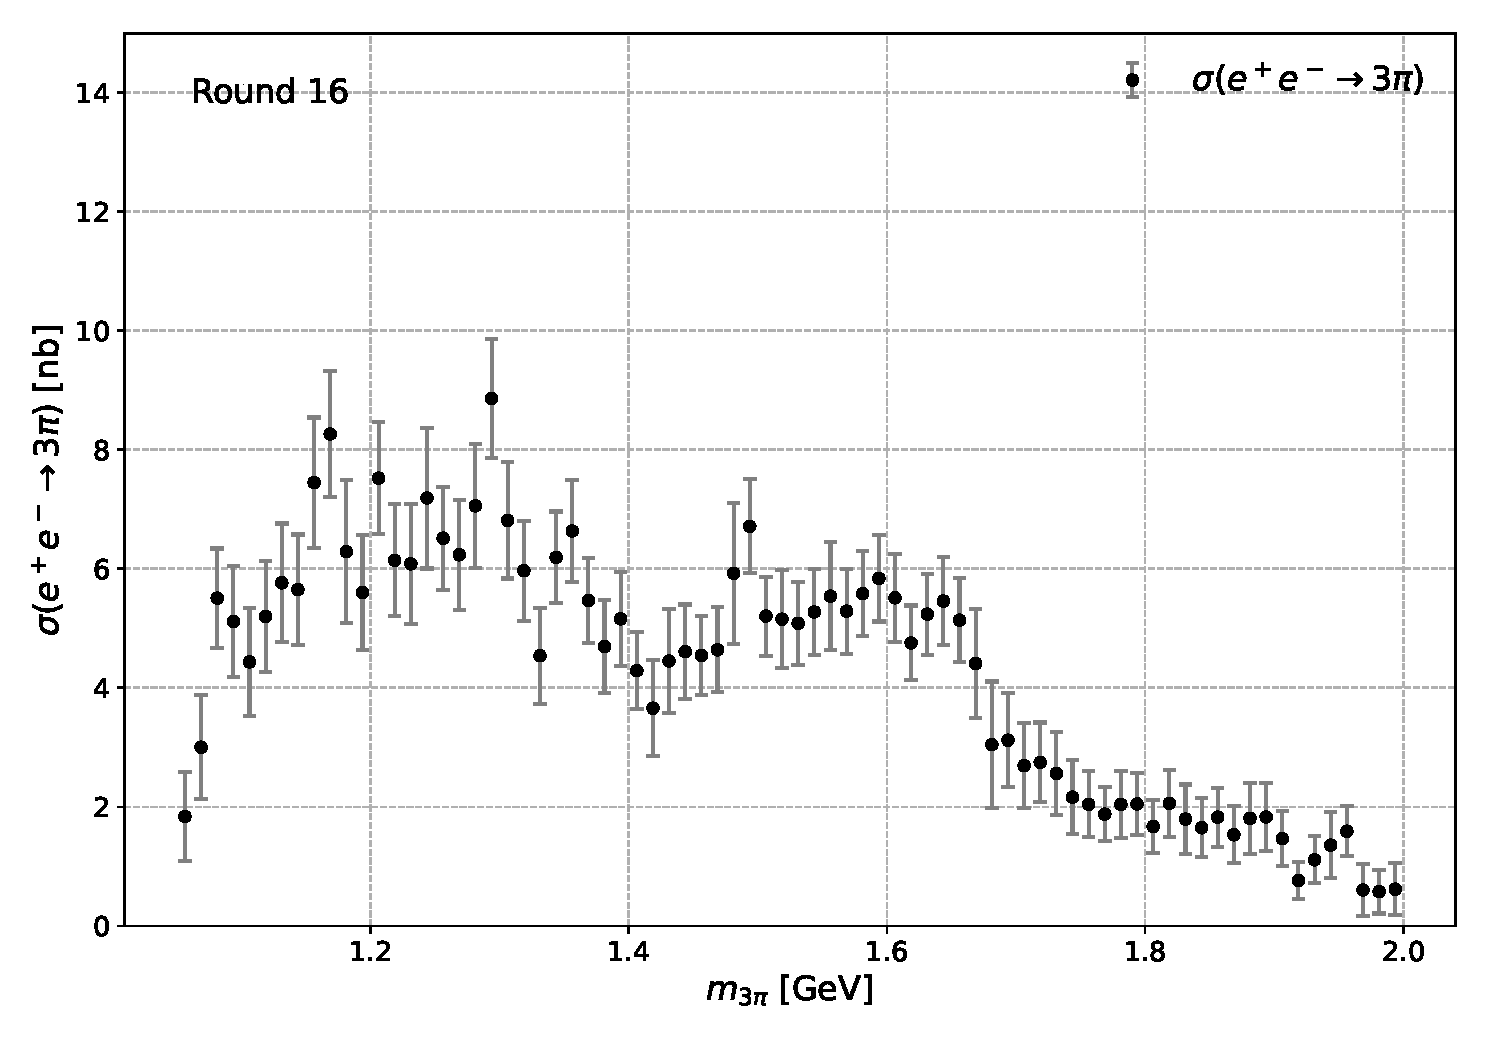
\includegraphics[width=0.32\textwidth]{fig/sigma_final_round16_high.eps}
        \label{fig:sigma_final_round16_high}
    }

    \vspace{0.5\baselineskip}

    % === Row 4: Round 17 ===
    \subfloat[Round 17, $\omega(782)$ region]{
        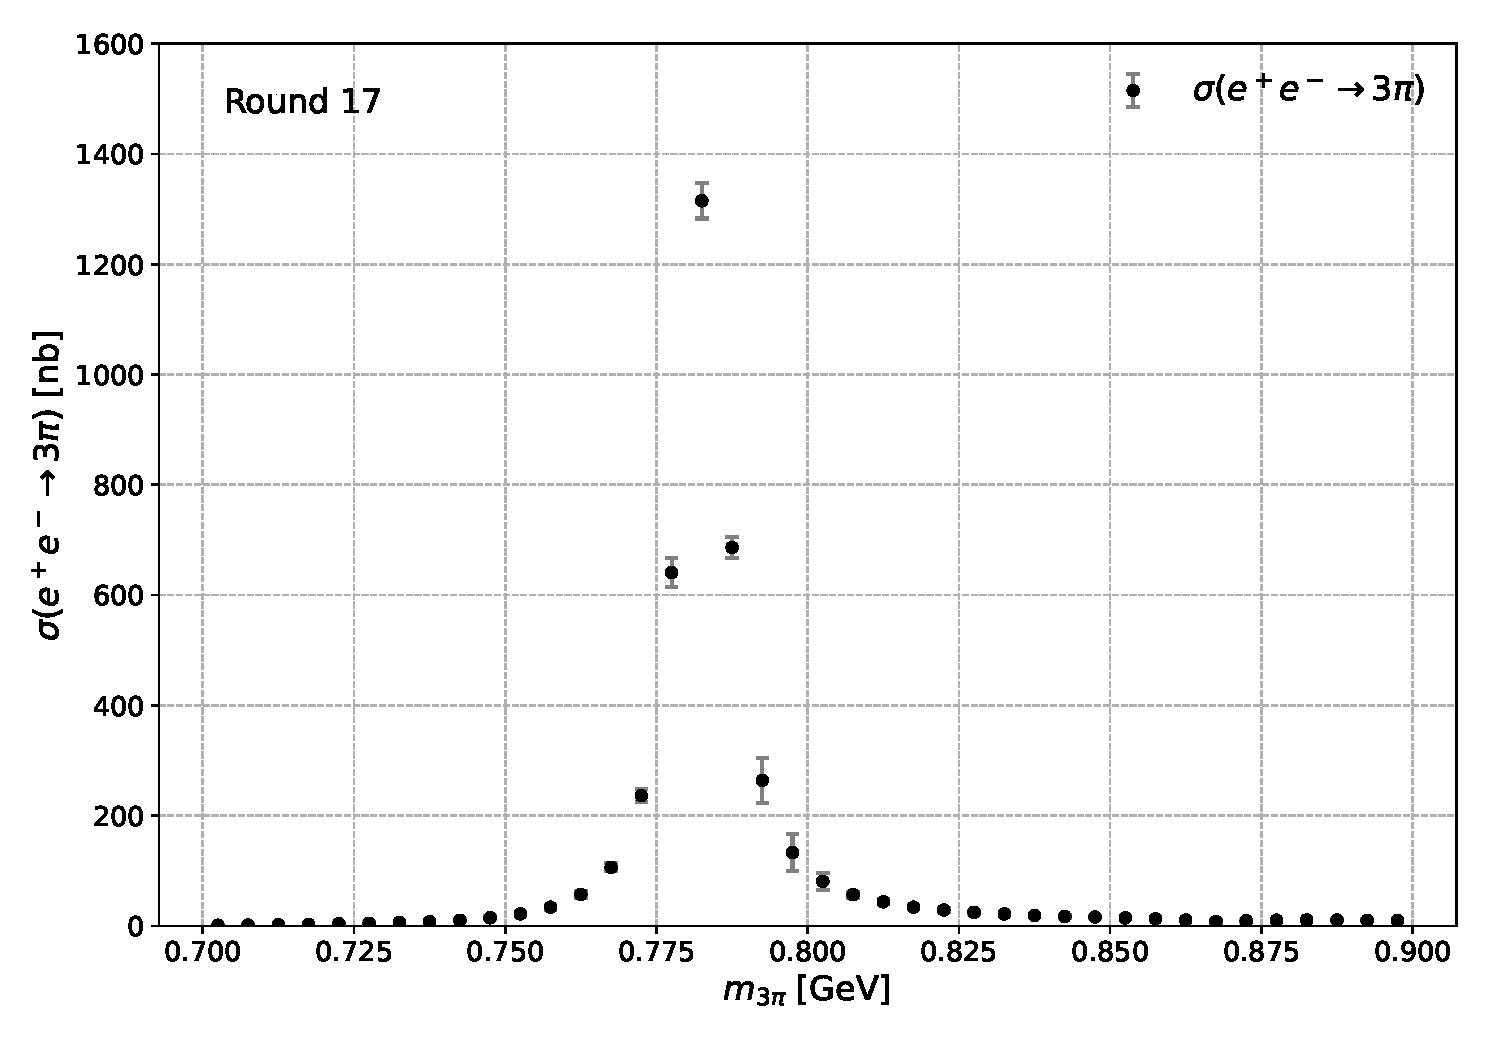
\includegraphics[width=0.32\textwidth]{fig/sigma_final_round17_omega.eps}
        \label{fig:sigma_final_round17_omega}
    }\hfill
    \subfloat[Round 17, $\phi(1020)$ region]{
        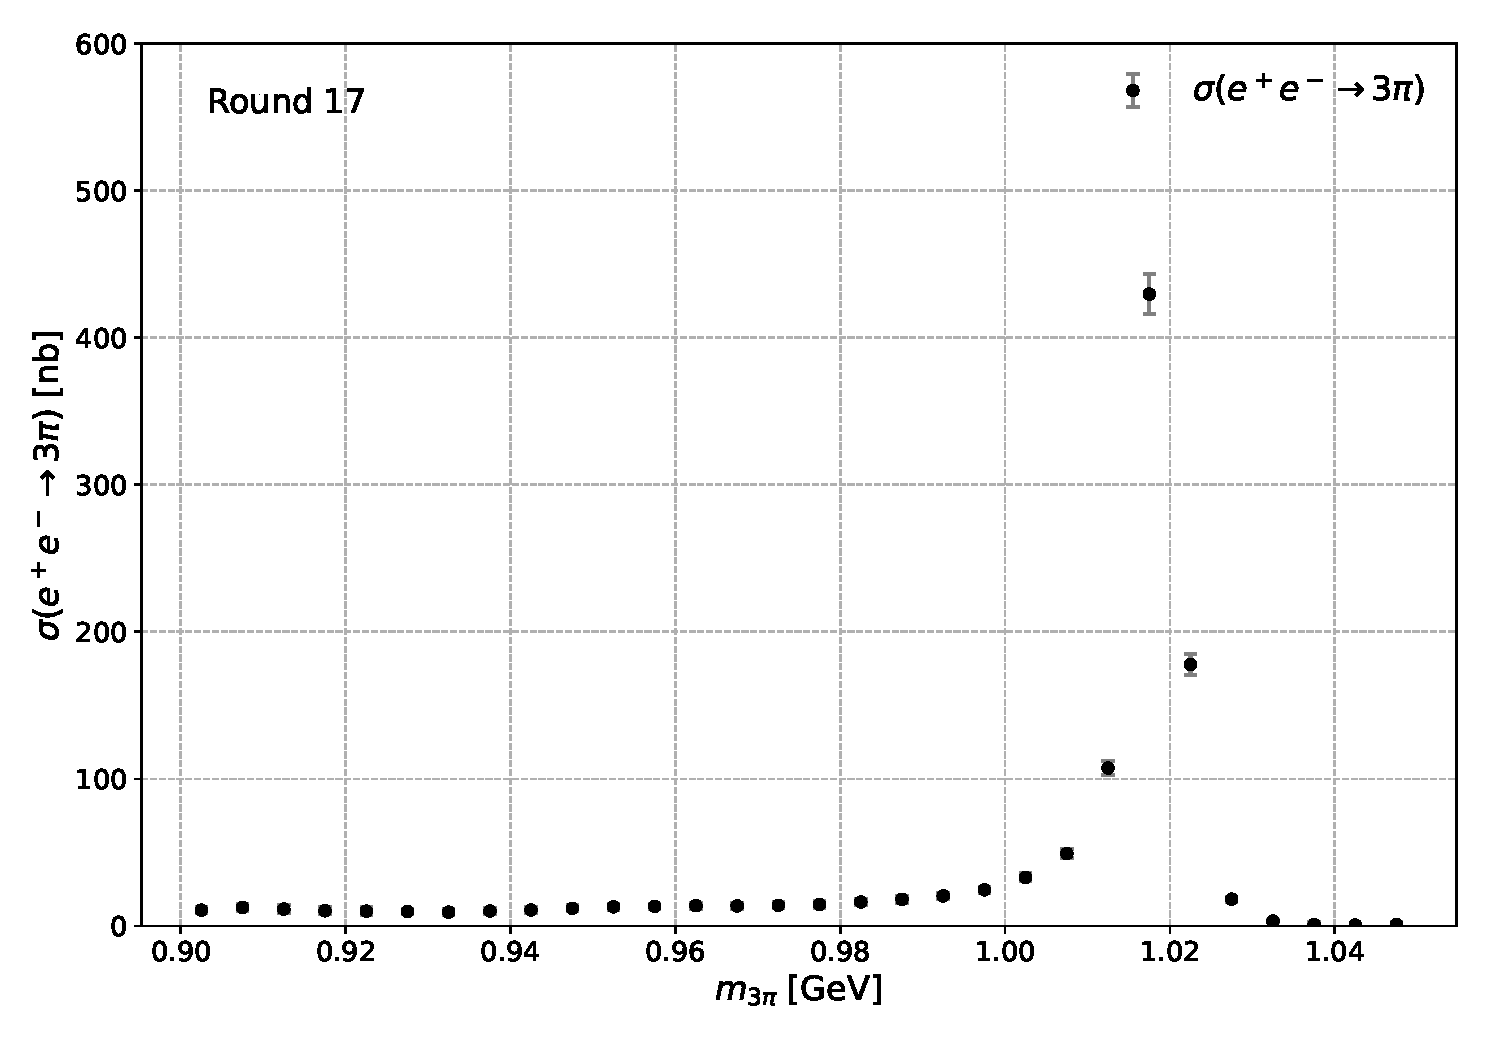
\includegraphics[width=0.32\textwidth]{fig/sigma_final_round17_phi.eps}
        \label{fig:sigma_final_round17_phi}
    }\hfill
    \subfloat[Round 17, $\omega^{\prime}/\omega^{\prime\prime}$ region]{
        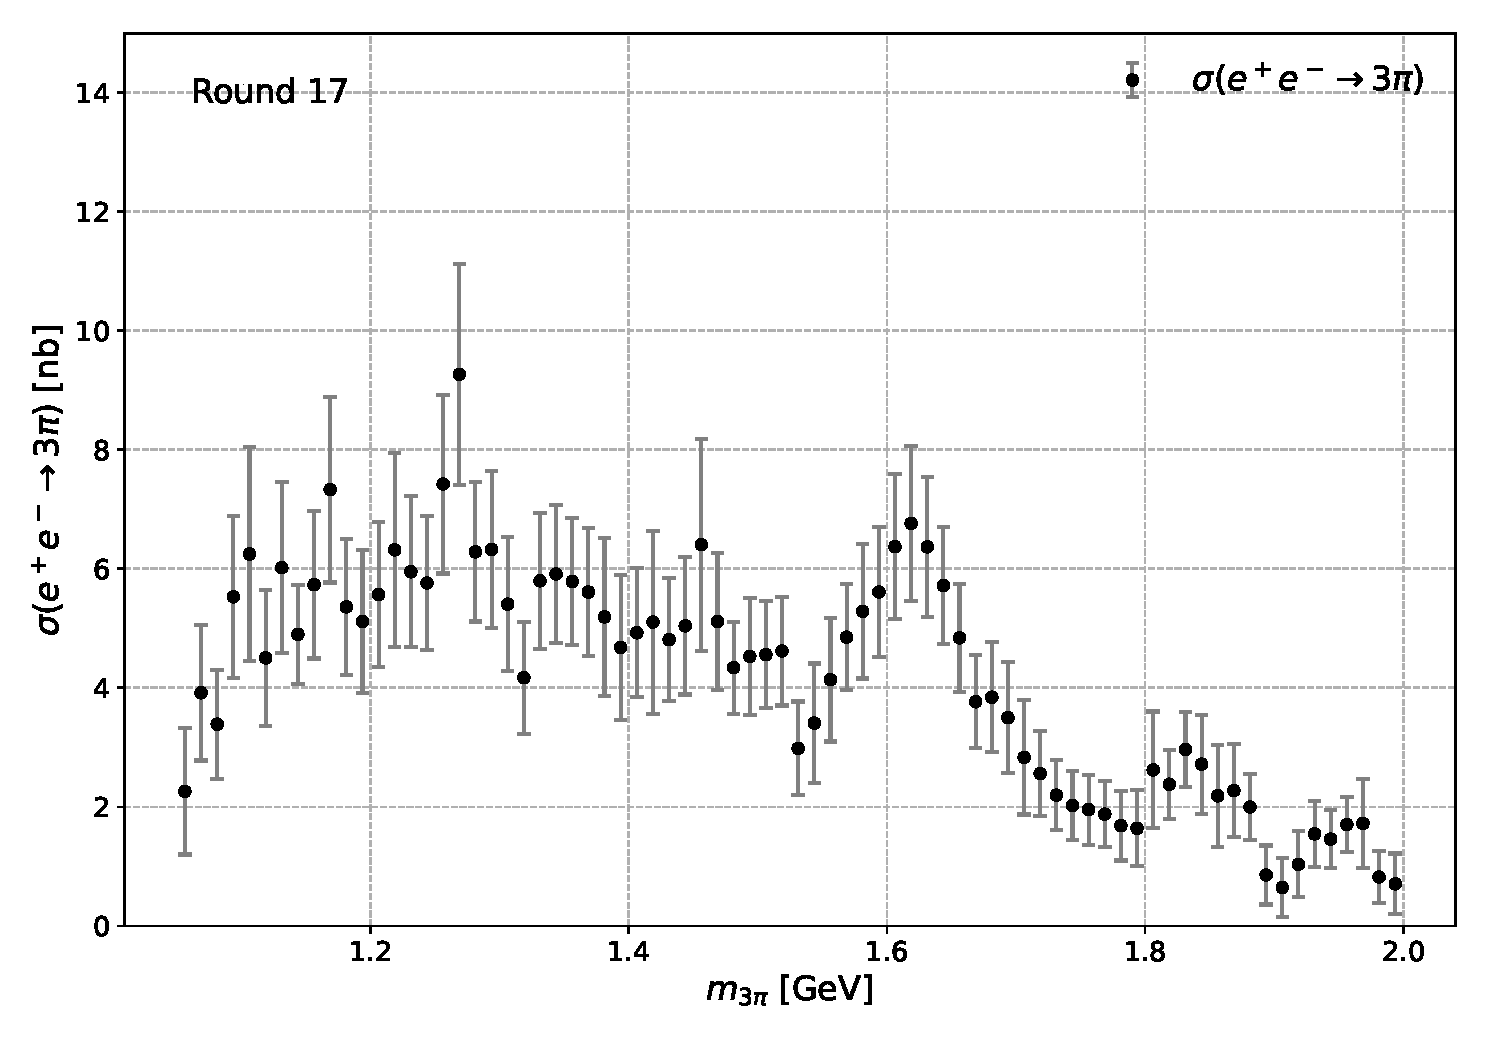
\includegraphics[width=0.32\textwidth]{fig/sigma_final_round17_high.eps}
        \label{fig:sigma_final_round17_high}
    }

    \caption{Dressed cross section $\sigma_{3\pi}^{\text{dress}}(m)$ results for the four independent data-taking periods (Round~03/04, Round~15, Round~16, and Round~17). The uncertainties are derived from the covariance matrices obtained from the unfolding procedure, which fully describe the correlations of the unfolded mass spectrum.}
    \label{fig:sigma_dress_results_all_rounds}
\end{figure}

\clearpage
\subsection{Combination of independent dressed cross section measurements}

Since the four data-taking periods (Round~03/04, Round~15, Round~16, and Round~17) are statistically independent, we can combine their dressed cross section results to obtain a more precise measurement. However, a simple weighted average using only the diagonal uncertainties would be suboptimal, as it neglects the bin-to-bin correlations within each measurement that arise from the unfolding procedure.

To properly account for these correlations, we employ the Best Linear Unbiased Estimator (BLUE) method~\cite{BLUE1,BLUE2}. BLUE provides a systematic framework for combining multiple correlated measurements that estimate the same underlying quantity, producing an estimate that is both unbiased and has minimum variance.

\subsubsection{Formalism of BLUE}

Suppose we have $n$ independent measurements $\mathbf{x}_i$ ($i = 1, \ldots, n$), each being a vector of length $m$ (corresponding to the $m$ invariant mass bins). Each measurement is an unbiased estimator of the true value $\boldsymbol{\mu}$:
\begin{equation}
    E[\mathbf{x}_i] = \boldsymbol{\mu}, \quad \text{Cov}(\mathbf{x}_i) = \mathbf{V}_i
\end{equation}
where $\mathbf{V}_i$ is the $m \times m$ covariance matrix for the $i$-th measurement, which contains both the variances ($\sigma_{i,p}^2$ on the diagonal) and the bin-to-bin covariances ($\rho_{pq}\sigma_{i,p}\sigma_{i,q}$ off-diagonal). Since the measurements are independent, the cross-covariances satisfy $\text{Cov}(\mathbf{x}_i, \mathbf{x}_j) = 0$ for $i \neq j$.

We seek a linear combination of all measurements:
\begin{equation}
    \hat{\boldsymbol{\mu}} = \sum_{i=1}^{n} \mathbf{W}_i \mathbf{x}_i
\end{equation}
where each $\mathbf{W}_i$ is an $m \times m$ weight matrix to be determined. The estimator $\hat{\boldsymbol{\mu}}$ is required to be unbiased:
\begin{equation}
    E[\hat{\boldsymbol{\mu}}] = \sum_{i=1}^{n} \mathbf{W}_i E[\mathbf{x}_i] = \left( \sum_{i=1}^{n} \mathbf{W}_i \right) \boldsymbol{\mu} = \boldsymbol{\mu}
\end{equation}
which imposes the constraint $\sum_{i=1}^{n} \mathbf{W}_i = \mathbf{I}$ (the identity matrix).

The covariance matrix of the combined estimator is:
\begin{equation}
    \mathbf{U} = \text{Cov}(\hat{\boldsymbol{\mu}}) = \sum_{i=1}^{n} \mathbf{W}_i \mathbf{V}_i \mathbf{W}_i^T
\end{equation}
since the cross-terms vanish due to independence.

\subsubsection{Optimal weights}

The BLUE method minimizes the variance (in the sense of matrix trace or any positive-definite metric) subject to the unbiasedness constraint. Solving this optimization problem using Lagrange multipliers yields the optimal weight matrices:
\begin{equation}
    \mathbf{W}_i = \left( \sum_{j=1}^{n} \mathbf{V}_j^{-1} \right)^{-1} \mathbf{V}_i^{-1}
\end{equation}
provided that all $\mathbf{V}_i$ are invertible. If some covariance matrices are singular or near-singular, we use the Moore-Penrose pseudo-inverse instead.

Substituting these weights back gives the combined estimate:
\begin{equation}
    \hat{\boldsymbol{\mu}} = \left( \sum_{i=1}^{n} \mathbf{V}_i^{-1} \right)^{-1} \left( \sum_{i=1}^{n} \mathbf{V}_i^{-1} \mathbf{x}_i \right)
    \label{eq:blue_estimate}
\end{equation}
and its covariance matrix:
\begin{equation}
    \mathbf{U} = \left( \sum_{i=1}^{n} \mathbf{V}_i^{-1} \right)^{-1}
    \label{eq:blue_covariance}
\end{equation}

\subsubsection{Application to this analysis}

We apply the BLUE method to combine the four independent measurements of $\sigma_{3\pi}^{\text{dress}}(m) \cdot \mathcal{B}(\pi^0\to\gamma\gamma)$, each represented by a vector $\mathbf{x}_i$ (size 40 for Region~1, 30 for Region~2, and 76 for Region~3) and its associated covariance matrix $\mathbf{V}_i$ obtained from the unfolding procedure via standard error propagation. The four $\mathbf{V}_i$ are derived from the covariance matrices of the unfolded mass spectra $\left( \frac{dN}{dm} \right)^{\text{gen}}$, scaled by the luminosity factors:
\begin{equation}
    \mathbf{V}_i = \frac{\mathbf{V}_i^{(N)}}{\Delta L_i^2}
\end{equation}
where $\mathbf{V}_i^{(N)}$ is the covariance matrix of the unfolded yield, and $\Delta L_i$ is the integrated luminosity per mass bin for the $i$-th period. Note that the branching fraction $\mathcal{B}(\pi^0\to\gamma\gamma)$ is intentionally omitted here, as it will be applied after the combination to allow for separate treatment of its systematic uncertainty.

The combined result $\hat{\boldsymbol{\mu}}_{\text{withBR}}$ therefore represents the best estimate of $\sigma_{3\pi}^{\text{dress}}(m) \cdot \mathcal{B}(\pi^0\to\gamma\gamma)$, with its covariance matrix $\mathbf{U}$ given by Eq.~(\ref{eq:blue_covariance}). The final dressed cross section is obtained by dividing by the central value of the branching fraction:
\begin{equation}
    \hat{\boldsymbol{\mu}}_{\text{dressed}} = \frac{\hat{\boldsymbol{\mu}}_{\text{withBR}}}{\mathcal{B}(\pi^0\to\gamma\gamma)}, \qquad
    \mathbf{U}_{\text{dressed}} = \frac{\mathbf{U}}{\mathcal{B}(\pi^0\to\gamma\gamma)^2}
\end{equation}
The covariance matrix $\mathbf{U}_{\text{dressed}}$ accounts for all statistical uncertainties propagated from the unfolding procedure. The systematic uncertainty due to the branching fraction is not included here and will be treated separately in Sec.~\ref{sec:sys_uncertainties}, as the final dressed cross section is not the ultimate physical quantity of interest in this analysis.

Figure~\ref{fig:blue_merged_results} shows the BLUE-combined dressed cross section results for the three invariant mass regions: the $\omega(782)$ region ($0.7-0.9$~GeV), the $\phi(1020)$ region ($0.9-1.05$~GeV), and the $\omega^{\prime}/\omega^{\prime\prime}$ region ($1.05-2.0$~GeV). The combined result exhibits significantly improved precision compared to individual measurements, particularly in the $\omega(782)$ region where the statistical uncertainties dominate.

\begin{figure}[htbp]
    \centering
    
    \subfloat[$\omega(782)$ region]{
        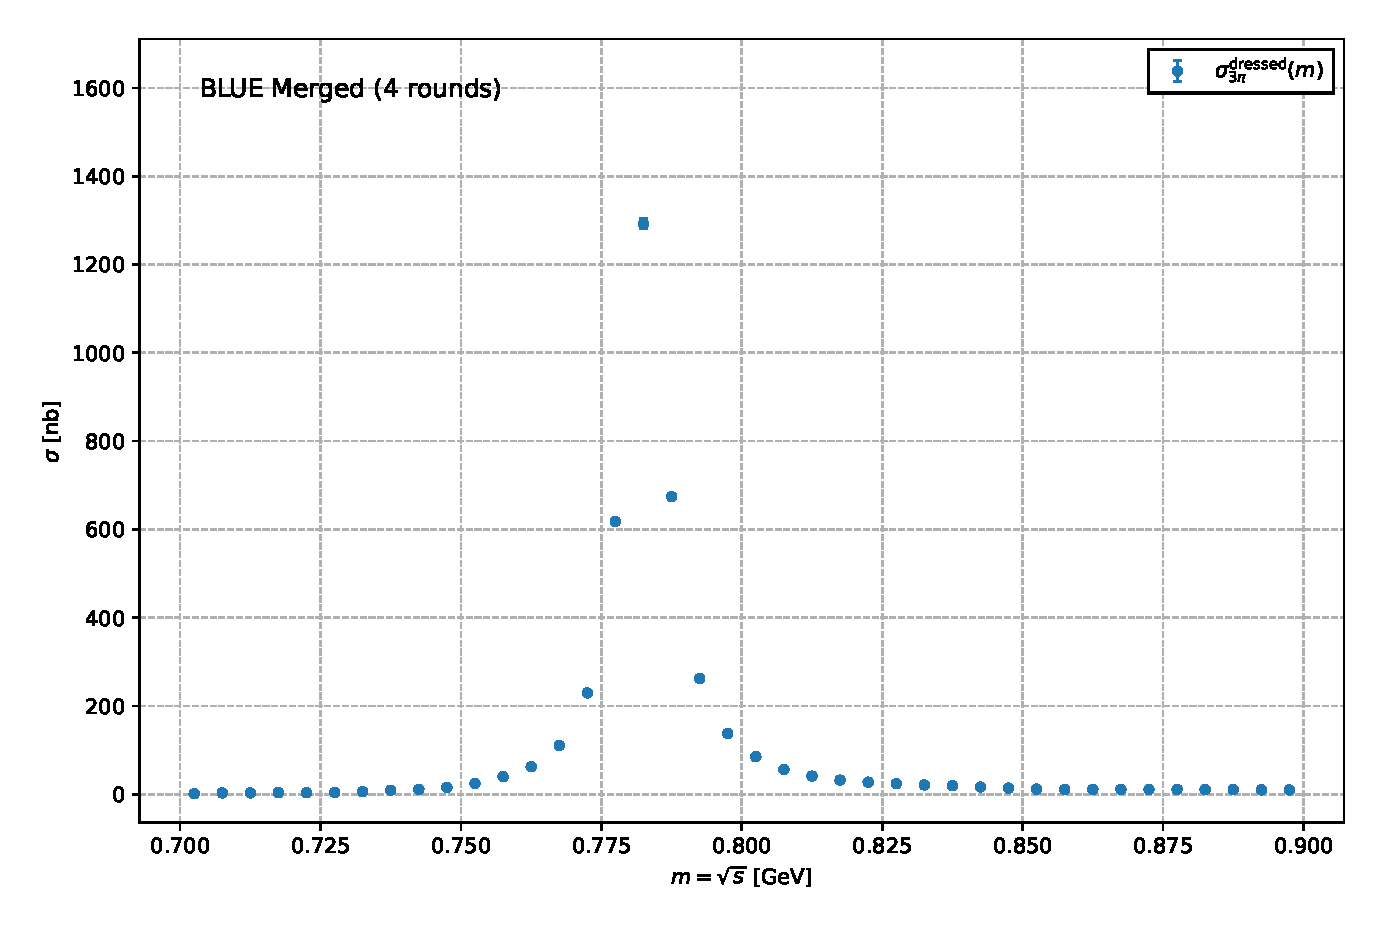
\includegraphics[width=0.32\textwidth]{fig/blue_merged_region1.eps}
        \label{fig:blue_merged_region1}
    }\hfill
    \subfloat[$\phi(1020)$ region]{
        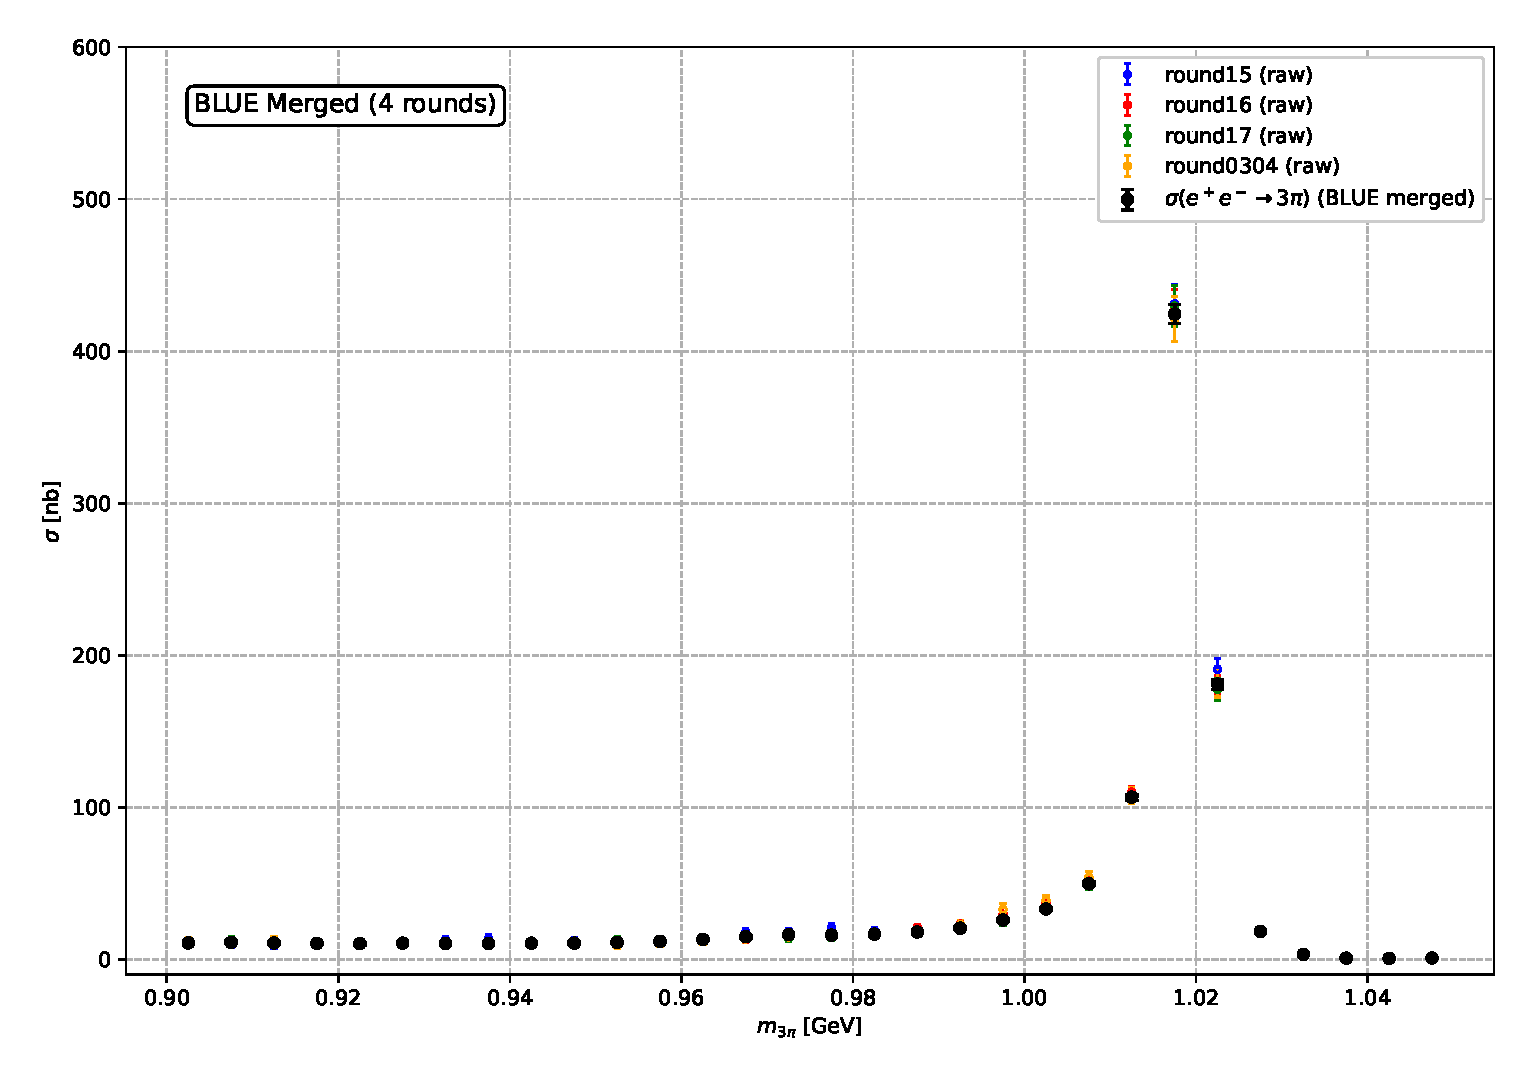
\includegraphics[width=0.32\textwidth]{fig/blue_merged_region2.eps}
        \label{fig:blue_merged_region2}
    }\hfill
    \subfloat[$\omega^{\prime}/\omega^{\prime\prime}$ region]{
        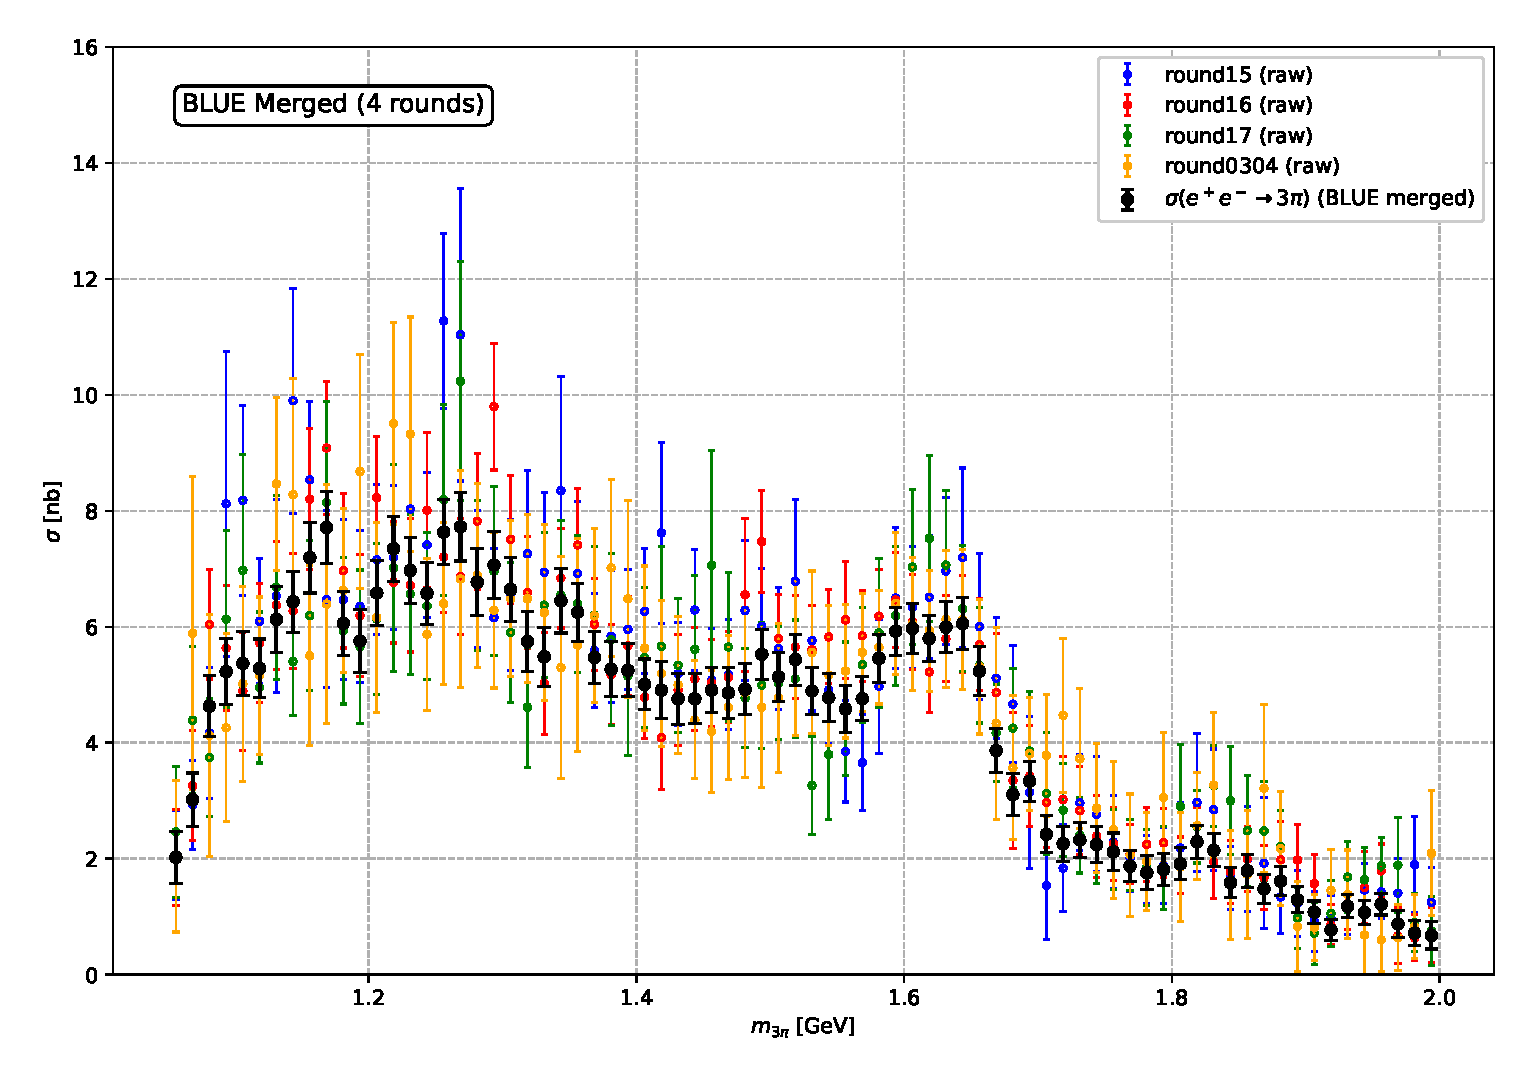
\includegraphics[width=0.32\textwidth]{fig/blue_merged_region3.eps}
        \label{fig:blue_merged_region3}
    }
    
    \caption{BLUE-combined dressed cross section $\sigma_{3\pi}^{\text{dress}}(m)$ results for the three invariant mass regions. The error bars represent the statistical uncertainties propagated from the covariance matrices. The combination significantly improves the statistical precision compared to any single data-taking period.}
    \label{fig:blue_merged_results}
\end{figure}

For completeness, Fig.~\ref{fig:blue_merged_all_regions} presents the combined results across all three regions on a logarithmic scale, illustrating the full spectrum from $0.7$ to $2.0$~GeV in a single view.

\begin{figure}[htbp]
    \centering
    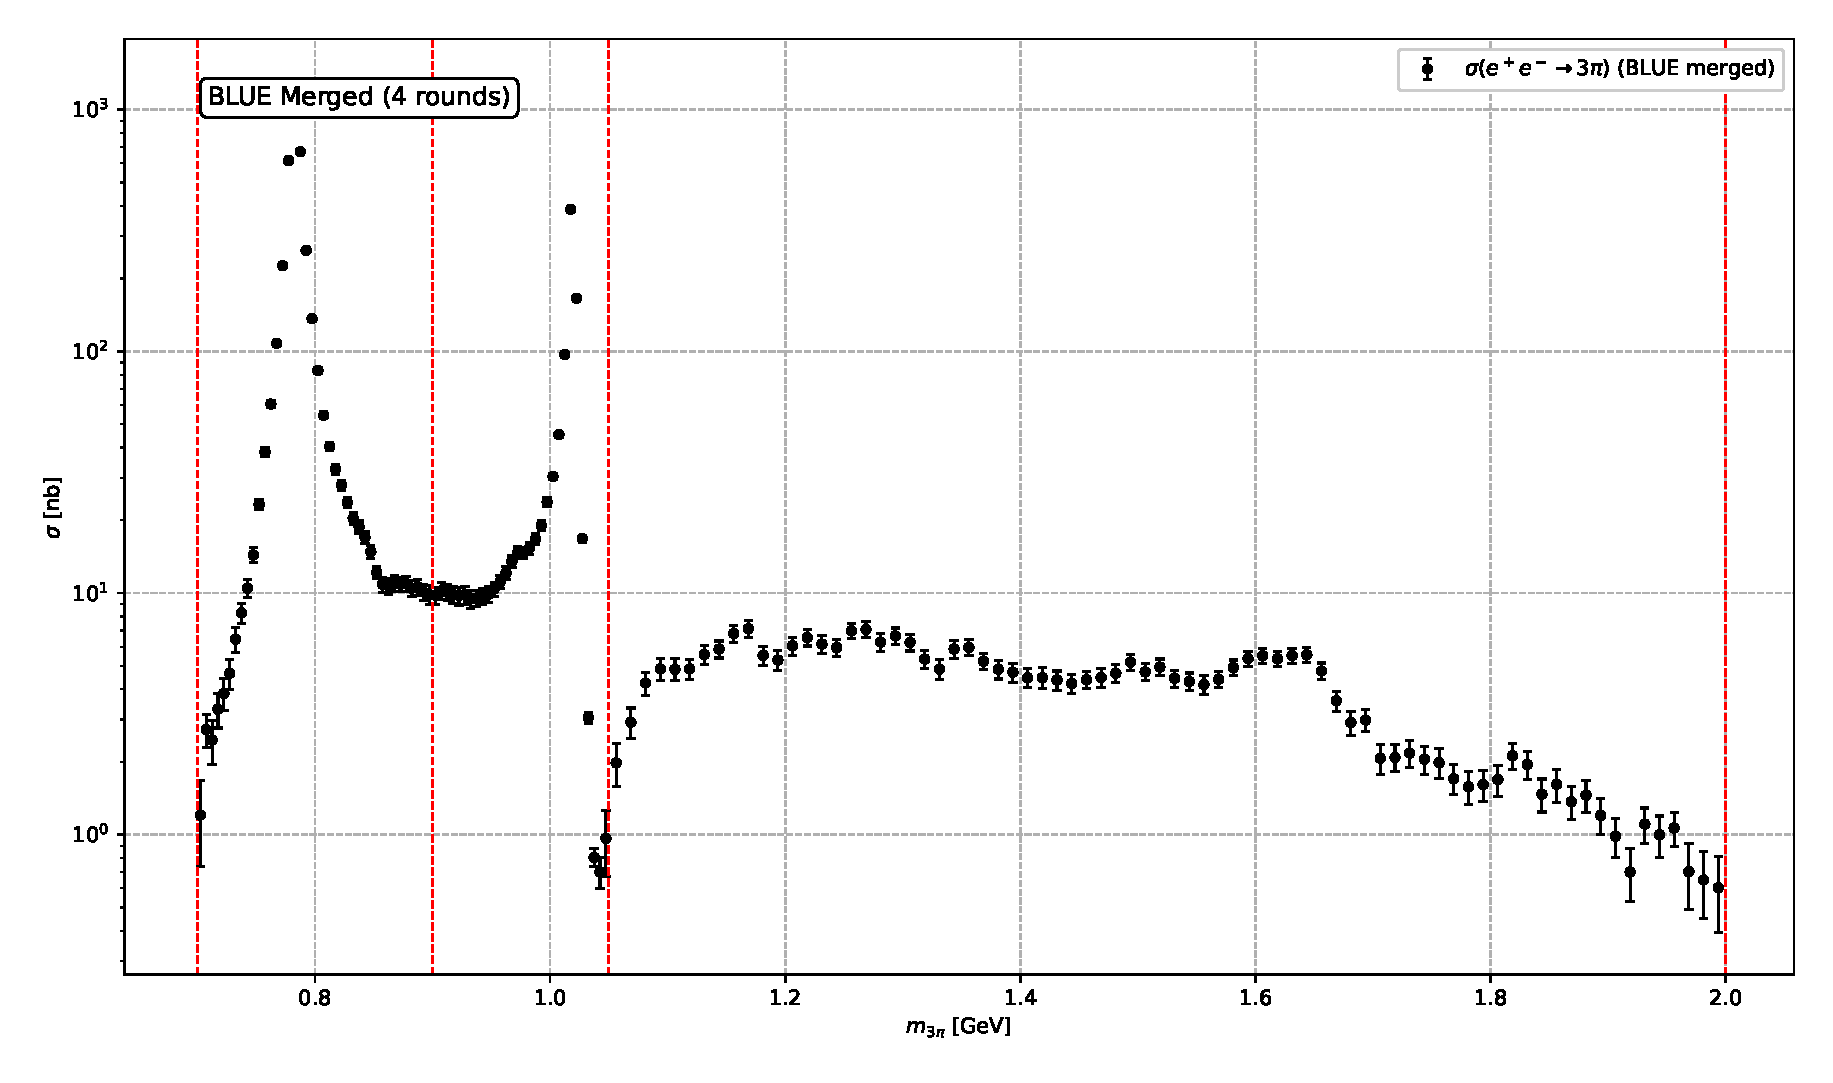
\includegraphics[width=0.75\textwidth]{fig/blue_merged_all_regions.eps}
    \caption{BLUE-combined dressed cross section $\sigma_{3\pi}^{\text{dress}}(m)$ across all three invariant mass regions, shown on a logarithmic scale.}
    \label{fig:blue_merged_all_regions}
\end{figure}

    \clearpage
    \begin{thebibliography}{99}

    %----------------------------1_introduction---------------------

    %----------------------------2_detector---------------------
    \bibitem{whitePaper}
    M. Ablikim \textit{et al.} (BESIII Collaboration),
    \emph{Future Physics Programme of BESIII},
    \emph{Chinese Phys. C} \textbf{44} (2020).

    \bibitem{Yang2014}
    R. X. Yang \textit{et al.},
    \emph{MRPC detector for the BESIII E-TOF upgrade},
    \emph{Journal of Instrumentation}, \textbf{Volume 9}, September 2014.
    \href{https://doi.org/10.1088/1748-0221/9/09/C09032}{DOI: 10.1088/1748-0221/9/09/C09032}.

    \bibitem{BESIII_detector}
    M.~Ablikim \textit{et al.} [BESIII],
    %\emph{Design and construction of the BESIII detector}, 
    %\emph{Nuclear Instruments and Methods in Physics Research Section A: Accelerators, Spectrometers, Detectors and Associated Equipment}, \textbf{Volume 614}, Issue 3, Pages 345-399, 11 March 2010. 
    \href{https://doi.org/10.1016/j.nima.2009.12.050}{DOI: 10.1016/j.nima.2009.12.050}.

    %----------------------------3_sample---------------------

    \bibitem{BESIII_lumi0304}
    M.~Ablikim \textit{et al.} [BESIII],
    %Measurement of the e+e− → π+π− cross section between 600 and 900 MeV using initial state radiation,
    %Physics Letters B, Volume 753, Pages 629-638, 2016.
    \href{https://doi.org/10.1016/j.physletb.2015.11.043}{DOI: 10.1016/j.physletb.2015.11.043}.

    \bibitem{BESIII_lumi_2024}
    M.~Ablikim \textit{et al.} [BESIII Collaboration],
    %Measurement of integrated luminosity of data collected at 3.773 GeV by BESIII from 2021 to 2024*,
    %Chinese Physics C, Volume 48, Number 12, Pages 123001, December 2024.
    \href{https://doi.org/10.1088/1674-1137/ad70a0}{DOI: 10.1088/1674-1137/ad70a0}.

    \bibitem{geant4}
    S.~Agostinelli \textit{et al.} [GEANT4],
    \href{https://doi.org/10.1016/S0168-9002(03)01368-8}{\emph{Nucl. Instrum. Meth. A} \textbf{506, 250-303 (2003)}}.


    %----------------------------4_selection---------------------

    %----------------------------7_summary---------------------

\end{thebibliography}

    \newpage
    \appendix
    \section*{APPENDIX}  % use *-form to suppress numbering
    % \input{Appendix_BDTG_REWEIGHTING.tex}
    \clearpage
\end{linenumbers}

\end{document}
